%
%
% UCSD Doctoral Dissertation Template
% -----------------------------------
% https://github.com/ucsd-thesis/ucsd-thesis
%
%
% ----------------------------------------------------------------------
% WARNING: 
%
%   This template has not endorced by OGS or any other official entity.
%   The official formatting guide can be obtained from OGS.
%   It can be found on the web here:
%   http://grad.ucsd.edu/_files/academic-affairs/Dissertations_Theses_Formatting_Manual.pdf
%
%   No guaranty is made that this LaTeX class conforms to the official UCSD guidelines.
%   Make sure that you check the final document against the Formatting Manual.
%  
%   That being said, this class has been routinely used for successful 
%   publication of doctoral theses.  
%
%   The ucsd.cls class files are only valid for doctoral dissertations.
%
%
% ----------------------------------------------------------------------
% GETTING STARTED:
%
%   Lots of information can be found on the project wiki:
%   http://code.google.com/p/ucsd-thesis/wiki/GettingStarted
%
%
%   To make a pdf from this template use the command:
%     pdflatex template
%
%
%   To get started please read the comments in this template file 
%   and make changes as appropriate.
%
%   If you successfully submit a thesis with this package please let us
%   know.
%
%
% ----------------------------------------------------------------------
% KNOWN ISSUES:
%
%   Currently only the 12pt size conforms to the UCSD requirements.
%   The 10pt and 11pt options make the footnote fonts too small.
%
%
% ----------------------------------------------------------------------
% HELP/CONTACT:
%
%   If you need help try the ucsd-thesis google group:
%   http://groups.google.com/group/ucsd-thesis
%
%
% ----------------------------------------------------------------------
% BUGS:
%
%   Please report all bugs at:
%   https://github.com/ucsd-thesis/ucsd-thesis/issues
%
%
% ----------------------------------------------------------------------
% More control of the formatting of your thesis can be achieved through
% modifications of the included LaTeX class files:
%
%   * ucsd.cls    -- Class file
%   * uct10.clo   -- Configuration files for font sizes 10pt, 11pt, 12pt
%     uct11.clo                            
%     uct12.clo
%
% ----------------------------------------------------------------------



% Setup the documentclass 
% default options: 12pt, oneside, final
%
% fonts: 10pt, 11pt, 12pt -- are valid for UCSD dissertations.
% sides: oneside, twoside -- note that two-sided theses are not accepted 
%                            by OGS.
% mode: draft, final      -- draft mode switches to single spacing, 
%                            removes hyperlinks, and places a black box
%                            at every overfull hbox (check these before
%                            submission).
% chapterheads            -- Include this if you want your chapters to read:
%                              Chapter 1
%                              Title of Chapter
%
%                            instead of
%                              1 Title of Chapter
\documentclass[12pt,chapterheads]{ucsd}

%packages added by vineet
\usepackage{subfigure}
\usepackage{verbatim}
\usepackage{textcomp} % for \textquotesingle
\usepackage{array}% for extended column definitions    
\usepackage{url} %for url in bib -- trying 
\usepackage{wrapfig} %for 0.5 length caption for figures
\usepackage{dirtytalk} %for quotes
%\usepackage[titles]{tocloft} %to remove dots in toc
% \renewcommand{\cftdot}{}
\newcommand{\Hair}{\ifmmode\mskip1mu\else\kern0.08em\fi} %forhairspace -- used as \Hair (no $$ needed)

% Include all packages you need here.  
% Some standard options are suggested below.
%
% See the project wiki for information on how to use 
% these packages. Other useful packages are also listed there.
%
%   http://code.google.com/p/ucsd-thesis/wiki/GettingStarted



%% AMS PACKAGES - Chances are you will want some or all 
%    of these if writing a dissertation that includes equations.
%  \usepackage{amsmath, amscd, amssymb, amsthm}

%% GRAPHICX - This is the standard package for 
%    including graphics for latex/pdflatex.
\usepackage{scrextend}
\usepackage{pslatex}
\usepackage{graphicx}

%% CAPTION
% This overrides some of the ugliness in ucsd.cls and
% allows the text to be double-spaced while letting figures,
% tables, and footnotes to be single-spaced--all OGS requirements.
% NOTE: Must appear after graphics and ams math
\makeatletter
\gdef\@ptsize{2}% 12pt documents
\let\@currsize\normalsize
\makeatother
\usepackage{setspace}
\doublespace
\usepackage[font=small, width=0.9\textwidth]{caption}

%% SUBFIG - Use this to place multiple images in a
%    single figure.  Subfig will handle placement and
%    proper captioning (e.g. Figure 1.2(a))
% \usepackage{subfig}

%% TIMES FONT - replacements for Computer Modern
%%   This package will replace the default font with a
%%   Times-Roman font with math support.
%\usepackage[T1]{fontenc}
%\usepackage{mathptmx}
%\usepackage{ebgaramond}  %vineet edit to change font
\usepackage{palatino}


%% INDEX
%   Uncomment the following two lines to create an index: 
% \usepackage{makeidx}
% \makeindex
%   You will need to uncomment the \printindex line near the
%   bibliography to display the index.  Use the command
% \index{keyword} 
%   within the text to create an entry in the index for keyword.
%   To compile a LaTeX document with an index the 'makeindex'
%   command will need to be run.  See the wiki for more details.

%% HYPERLINKS
%   To create a PDF with hyperlinks, you need to include the hyperref package.
%   THIS HAS TO BE THE LAST PACKAGE INCLUDED!
%   Note that the options plainpages=false and pdfpagelabels exist
%   to fix indexing associated with having both (ii) and (2) as pages.
%   Also, all links must be black according to OGS.
%   See: http://www.tex.ac.uk/cgi-bin/texfaq2html?label=hyperdupdest
%   Note: This may not work correctly with all DVI viewers (i.e. Yap breaks).
%   NOTE: hyperref will NOT work in draft mode, as noted above.
% \usepackage[colorlinks=true, pdfstartview=FitV, 
%             linkcolor=black, citecolor=black, 
%             urlcolor=black, plainpages=false,
%             pdfpagelabels]{hyperref}
% \hypersetup{ pdfauthor = {Your Name Here}, 
%              pdftitle = {The Title of The Dissertation}, 
%              pdfkeywords = {Keywords for Searching}, 
%              pdfcreator = {pdfLaTeX with hyperref package}, 
%              pdfproducer = {pdfLaTeX} }
% \urlstyle{same}
% \usepackage{bookmark}


%% CITATIONS
% Sets citation format
% and fixes up citations madness
\usepackage{microtype}  % avoids citations that hang into the margin

%% FOOTNOTE-MAGIC
% Enables footnotes in tables, re-referencing the same footnote multiple times.
\usepackage{footnote}
\makesavenoteenv{tabular}
\makesavenoteenv{table}


%% TABLE FORMATTING MADNESS
% Enable all sorts of fun table tricks
\usepackage{rotating}  % Enables the sideways environment (NCPW)
\usepackage{array}  % Enables "m" tabular environment http://ctan.org/pkg/array
\usepackage{booktabs}  % Enables \toprule  http://ctan.org/pkg/array


\begin{document}

%% FRONT MATTER
%
%  All of the front matter.
%  This includes the title, degree, dedication, vita, abstract, etc..
%  Modify the file template_frontmatter.tex to change these pages.
%
%
% UCSD Doctoral Dissertation Template
% -----------------------------------
% http://ucsd-thesis.googlecode.com
%
%


%% REQUIRED FIELDS -- Replace with the values appropriate to you

% No symbols, formulas, superscripts, or Greek letters are allowed
% in your title.
\title{Social Computing with Procedural Guidance for Complex Work}

\author{Vineet Pandey}
\degreeyear{2019}

% Master's Degree theses will NOT be formatted properly with this file.
\degreetitle{Doctor of Philosophy}

\field{Computer Science \& Engineering}
%\specialization{Human-Computer Interaction}  % If you have a specialization, add it here

\chair{Professor Scott R. Klemmer}
% Uncomment the next line iff you have a Co-Chair
% \cochair{Professor Cochair Semimaster}
%
% Or, uncomment the next line iff you have two equal Co-Chairs.
%\cochairs{Professor Chair Masterish}{Professor Chair Masterish}

%  The rest of the committee members  must be alphabetized by last name.
\othermembers{
Professor James D. Hollan\\
Professor Laurel Riek\\
Professor Robin Knight\\
Professor Donald Norman\\
}
\numberofmembers{5} % |chair| + |cochair| + |othermembers|


%% START THE FRONTMATTER
%
\begin{frontmatter}

%% TITLE PAGES
%
%  This command generates the title, copyright, and signature pages.
%

\makefrontmatter

%% DEDICATION
%
%  You have three choices here:
%    1. Use the ``dedication'' environment.
%       Put in the text you want, and everything will be formated for
%       you. You'll get a perfectly respectable dedication page.
%
%
%    2. Use the ``mydedication'' environment.  If you don't like the
%       formatting of option 1, use this environment and format things
%       however you wish.
%
%    3. If you don't want a dedication, it's not required.
%
%
\begin{dedication}
  To the adventure of life
\end{dedication}


% \begin{mydedication} % You are responsible for formatting here.
%   \vspace{1in}
%   \begin{flushleft}
% 	To me.
%   \end{flushleft}
%
%   \vspace{2in}
%   \begin{center}
% 	And you.
%   \end{center}
%
%   \vspace{2in}
%   \begin{flushright}
% 	Which equals us.
%   \end{flushright}
% \end{mydedication}



%% EPIGRAPH
%
%  The same choices that applied to the dedication apply here.
%
\begin{epigraph} % The style file will position the text for you.
  \emph{I don't do it for the 'Gram,\\
	 I do it for Compton}\\
  ---Kendrick Lamar
%, ELEMENT., {\it DAMN}
\end{epigraph}

% \begin{myepigraph} % You position the text yourself.
%   \vfil
%   \begin{center}
%     {\bf Think! It ain't illegal yet.}
%
% 	\emph{---George Clinton}
%   \end{center}
% \end{myepigraph}


%% SETUP THE TABLE OF CONTENTS
%
\tableofcontents
\listoffigures  % Comment if you don't have any figures
\listoftables   % Comment if you don't have any tables



%% ACKNOWLEDGEMENTS
%
%  While technically optional, you probably have someone to thank.
%  Also, a paragraph acknowledging all coauthors and publishers (if
%  you have any) is required in the acknowledgements page and as the
%  last paragraph of text at the end of each respective chapter. See
%  the OGS Formatting Manual for more information.
%
\begin{acknowledgements}

%from gut instinct
We thank all participants who used Gut Instinct and pro-vided feedback. We thank members of Design Lab, espe-cially Steven Dow and Derek Lomas, and Michael Bern-stein for their useful comments on this work. We thank Brian Soe and Aliff Macapinlac for help developing the Gut Instinct website and running pilot studies. A Google Re-search Award and gift from SAP helped support this work.

%from docent
We thank Docent participants for their feedback. We thank Chen Yang, Cody Doan, and Aliyah Clayton for help developing the website and running pilot studies. We thank Anupriya Tripathi and Nicolai Reeve for finding relevant scientific resources for the site, and Madeleine Ball for introducing Docent to the Open Humans community. A Google Research Award and gift from SAP helped support this work.

\end{acknowledgements}


%% VITA
%
%  A brief vita is required in a doctoral thesis. See the OGS
%  Formatting Manual for more information.
%
\begin{vitapage}
\begin{vita}
  \item[2011] B.~Engineering. in Computer Science \emph{cum laude}, Birla Institute of Technology \& Science, Pilani, India
  \item[2016] M.S.in Computer Science \& Engineering, University of California San Diego
  \item[2019] Ph.~D. in Computer Science \& Engineering, University of California San Diego
\end{vita}S
\begin{publications}
  \item Your Name, ``A Simple Proof Of The Riemann Hypothesis'', \emph{Annals of Math}, 314, 2007.
  \item Your Name, Euclid, ``There Are Lots Of Prime Numbers'', \emph{Journal of Primes}, 1, 300 B.C.
\end{publications}
\end{vitapage}


%% ABSTRACT
%
%  Doctoral dissertation abstracts should not exceed 350 words.
%   The abstract may continue to a second page if necessary.
%
\begin{abstract}
  This dissertation will be abstract.
\end{abstract}


\end{frontmatter}






%% DISSERTATION

% A common strategy here is to include files for each of the chapters. I.e.,
% Place the chapters is separate files: 
%   chapter1.tex, chapter2.tex
% Then use the commands:
%   %%%%%%%%%%%%%%%%%%%%%%%%%%%%%%%%%%%%%%%%%%%%%%%
%\chapter{Scaffolding Citizen-led Complex Knowledge Work}
\chapter{Social Computing for Complex Knowledge Work}

\begin{quote}
\emph{This dissertation explores how the following things happen. Complex work is hard. Needs learning. People do things in groups. Social computing misses learning (learning is around but not here). why your title is what it is, what that means, how you set up your arguments, and what claims your introductory chapter makes. Current online platforms (like Facebook) are built on insights from psychology about capturing people’s attention. My research instead takes a more socially responsible approach by integrating learning theory and collaboration for people to perform complex work such as generating and evaluating scientific theories. This has the potential to diversify the stakeholders and contributors to our future society.}
\end{quote}
\vspace{0.25in}

Social computing platforms have revolutionized how most people connect, communicate, and share. We increasingly connect with friends and strangers in different ways for a number of purposes. Friends and family can stay in constant touch with their loved ones. Strangers from different parts of the world discuss their ideas about their health. Increasingly, these connection opportunities have also translated to more active doing: people fund other's\'  ideas that traditional business places might balk at. Some have used social platforms to amplify their voice and bring about social changes. for instance, people in Sudan have taken down dictators [??]. By transforming how we communicate, share, and chat, social computing has become perhaps the greatest internet-fueled change of our times. 

%%interactive vis (social computing discussions) is awesome
% people can do stuff with hypotheses (test them?)
%    however, viz is hard (scientific work)
%        programming toolkits needed and impose burden (support needed to get started, reduce burden, and …)

However, the benefits of social computing are not distributed equally. While everyone has a voice, some have bigger loudspeakers than others: xx\% of most popular posts are from experts. While anyone can organize and bring changes, collective attempts to organize frequently fail. While anyone can learn from widely accessible research papers and articles, people create faulty insights from self-tracking and conspiracy theories abound. With this lens, social computing seems less transformative but rather a highly scaled up version of the offline reality of limited expertise people live in. 
% 1 to 1 link with the first para

%\subsection{Pivot to people - People can do great things but need help...}
%Well, what are people good at? What are they motivated to do? 

%People have complementary knowledge in comparison to experts and are uninfected by expert biases; these insights are drawn from lived experience, both individual and collective.

Specific to this dissertation: While social computing platforms have vastly succeeded at keeping people engaged and sharing, they barely support \textit {citizen-led enquiry}. People have strong personal motivations and contextual insights. People possess a remarkable ability to identify patterns and create theories from their experiences [??]. While most people have an amazing breadth and depth of ideas, they lack the expertise to implement these ideas. To create knowledge, they need mental scaffolds for organizing complex work, domain knowledge to compose and execute the steps, and ways to ask for help. Experts benefit from conceptual knowledge, professional training, pre-existing organizational structure for collaboration, and direct access to resources. Currently, citizens lack these resources. social computing platforms where people spend ridiculous times provide little support. 

%this is the current state --  this is the big challenge, why is it a challenge
%% however, scaling good teaching is hard - kulkarni
%     this peer thing can be helpful (evidence from small studies)
%        however, this is challenging — 2 causes
%        interfaces need to provide scaffolding 


\begin{figure}[b] 
  \centering
  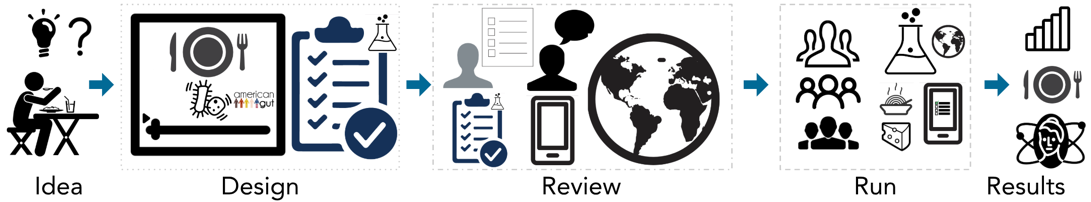
\includegraphics[width=1.0\textwidth]{figures/intro/intro-1}
  \caption[]
{The Gut Instinct platform enables anyone to transform their intuitions to hypotheses 
and then design and run experiments to test them [xx-xx]. Gut Instinct integrates 
conceptual learning embedded via short lectures and software-guided procedural 
learning to enable designing and reviewing experiments. Participants from around
 the world join experiments, follow instructions, and pro-vide data in response to 
automated data collection reminders. }
  \label{fig:intro-1}
\end{figure}

Consequently, this is unfortunate missed opportunity for both individuals and the world at large. Enabling peoplt to learn to perform personally meanignful work can help them answer their own questions. People's ideas can catalyze creating new knowledge that we are missing out on.  How might online systems support citizen-led knowledge work? 

Let''s reflect on this dual nature:  science can answer life-relevant questions but few know how to even get started. As a result, people fail to answer their questions and institutional science misses out on ideas from beyond the ivory tower. 

%one line to summarize my work -- see other intro

%two properties of classes help us - kulkarni
%this thesis leverages these two properties and provides a new class of benefits etc... 

%what helps us
%1. the scientific method is structured
%    1. even though creative and open-ended
%2. roles: people take them online
%    1. captures diversity — breadth
%    2. micro-expertise supports this explicitly 
%3. procedural learning: can teach people how to do things
%    1. captures learning — depth


This dissertation advances the design of social computing systems by integrating learning and collaboration to enable complex work such as generating and evaluating scientific theories. Over 600 people from 30 countries have self-organized to generate theories about the human microbiome and test them by running experiments. This dissertation raises the question: how can global communities create knowledge that meets their goals without waiting for experts to lead? 

Gut Instinct emodies this insight and introduces a collaborative citizen science platform for people to transform lived exes into scientific theories. 

%%%%%%%%%%%%%%%%%%%%%%%%%%%%%%
\section {People already do great things but struggle with complex tasks}

\subsection{People are awesome}
People design, build, and track to better understand and improve their health [?? dana lewis].  On numerous online fora, people share their intuitions, observations, folk theories, and even results from trying different approaches to improve their health, e.g. from simple ideas like ‘giving up drinking coffee to improve quality of sleep’ to tests and dietary approaches. People draw ideas from current research by reading and discussing papers. In many cases, these discussions are not just anecdotal but also derive from state-of-the-art scientific work. In some cases, people contribute back to scientific work as well.How can social computing platforms effectively enable people to do more personally meaningful work built upon their experiences and insights?

People’s curiosity, needs, and possibilities to do useful work is endless; however, traditional online systems don’t support them. Online fora encourage long, rambling discussions. Online learning provides conceptual lessons but people drop out and these are not linked to people’s needs.While learning resources like MOOCs abound, they hardly meet the need: many drop out, the lectures focus on conceptual knowledge, and lack the feedback needed to perform open-ended creative work. We know little about integrating learning resources and social computing affordances are far from each other. Moreover, currently both learning and work are not personal; can we change this? Lack of appropriate "learning abstractions" make complex work unrealistic.

The goal is to create environments for learning and collaboration through complex, personally meaningful work.

%%%%%%%%%%%%%%%%%%%%%%%%%%%%%%%%%%%%%%%%%%%%%%%%%%%
\subsection{Challenge: People' don't know what to do and how to do it}
Citizens have a different background than professional scientists; they have unique
 personal experiences but lack the years of domain training. Two major issues in 
enabling complex work on the internet are (diversity and scale?) 
quality of individual contribution and managing overall contributions from the crowd.
We desire social computing techniques that reliably enable a wide variety of people to 
contribute more than they naturally could and that manage the dependencies among
 a large set of tasks.

To create computational systems that leverage their strengths and mitigate the lack of training, this dissertation 
focuses on domains where the science is nascent, highly contextual, and personally motivating.
 Synthesizing the crowdsourcing literature and my experience highlights three challenges: 
poor signal-to-noise from crowds due to lack of training; inefficient collaboration without 
careful attention; and poor results (or no results at all) unless experts lead. 

To address  these concerns,  this dissertation introduces and evaluates peer production architectures 
and procedural learning.

\subsection{Scientific experimentation: An instance of complex knowledge work}
%here''s an example: experimentation 
Supporting complex knowledge work has been a challenge for Human Computer Interaction
 research (make specific). For instance, many people are interested in understanding and 
improving their health. Millions of peple from all over the world share their insights. 
Can't they run experiments for these?

Scientific experimentation features technical requirements and contextual choices 
that are inscrutable for a lay individual yet necessary for success [??]. While 
professional scientists and commercial ventures run experiments every day, with 
notable exceptions [??], empirical papers from non-professionals are 
vanishingly rare. This biases the questions asked, studies run, and knowledge 
created [??]. People have questions about their health, but lack the expertise 
and resources to scientifically investigate them. Broadening the pool of 
experimenters could help people investigate their curiosities, develop solutions 
to improve health and performance, and assist institutional researchers.


\textit{People lack the expertise to know what to do and how to do it.}. 
Success with complex creative activities requires procedural
knowledge (how to do things) in addition to conceptual
knowledge (facts). While many resources offer facts, procedural
learning is often ignored.The converse also holds, and much more often: novices are also
“uninfected” by all the knowledge that enables experts to
innovate.Sometimes, having a different background than experts can
be beneficial. Shared knowledge is great when it’s right, but
blocks progress when wrong. When false assumptions limit
experts, at least some novices are likely to be “uninfected”.
For example, GalaxyZoo volunteers discovered ‘green pea’
galaxies overlooked by scientists who mistakenly assumed
the green hue was merely an imaging artifact [54]. 


% kulkarni -- "This assessment requires bothcommon-sense knowledge to understand student work and the expertise to assess tacit criteria such as “well-designed” or “well-modularized” that cannot be completely articulated. Indeed, teaching such tacit criteria is an important goal in open-ended domains like design"


\textit{People lack a professional network to improve their work}. 
Furthermore,  how do people ask others for help? Who do they reach out to?

People are connected online and collectively have access to many resources.
In a large distributed community, there’s often someone who happens to 
have important relevant knowledge, usually drawing on a relevant but 
distant domain. Such distributed efforts are a type of lead-user innovation [31]. 
Having many people work on the same problem increases the odds that 
one will break through. Drawing on secondary expertise as inspiration can
 be an important agent of creativity because almost by definition, the 
combination is rare [10]. %Open \& crowd innovation builds up on contributions
 by diverse online participants, and a ‘bubbling up’ process for strong ideas [56].

While many hands make light work, novices need clear contribution opportunities. 
The crowdsourcing literature offers many good verification approaches for tasks 
with clear right or wrong answers – like whether two images represent the same 
product or what street number is written on a sign. However, verifying knowledge
 work necessitates a different approach because it requires making 
situationally-appropriate choices. 

%%%%%%%%%%%%%%%%%%%%%%%%%%%%%%%%%%%%%%%%%%%%%%%
\section{Thesis Statement and Contributions}
\noindent This dissertation investigates the question: how to enable people to perform personally meaningful work otherwise beyond their expertise? Underlying these investigations is the thesis:
%"My thesis statement is"
\begin{quote}
\emph{Providing task-specific guidance in social computing enables personally meaningful \& useful scientific work}
\end{quote}

This dissertation\textquotesingle s primary contribution is the idea of intergrating learning in social computing to enable groups of novices to perform complex, creative activities. The thesis achieves this integration by building a sequence of interactive prototypes that enable people to collaboratively generate and test hypotheses. In the process, the prototypes divide complex work into distinct activities: self-sourcing the design and crowdsourcing people''s inputs and data. Every prototype advances social computing further as a domain for deep, personally meaningful work. Beyond introducing learning abstractions, this dissertation carefully designs the affordances, support, and system to enable different users for different needs. 

 %To realize this idea, 
This dissertation makes three types of contributions: theoretical perspectives/techniques, real-world systems, and outcomes including empirical results, systems lessons, and dataset (Figure \ref{fig:contributions}). 

%%%%%%%%%
\subsection{Theoretical  Techniques}
Improving  work quality in social computing suggests deepening individual contributions and broadening participation by providing different contribution mechanisms.The former requires better learning tools and the latter requires better collaboration tools and dependency management. Consequently, this thesis' theoretical contributions include 1) principles to integrate guidance for complex tasks, and 2) ways to divide complex tasks into multiple roles or affordances.

%“..adapts and extends techniques from xxx” -  arvind

%system-led learning vs people-led
Traditional systems think of knowledge as being provided by the people, while we being the knowledge from the system itself.

%todo-introduce the learning and collaboraiton taxonomy here
\begin{figure}[b] 
  \centering
%  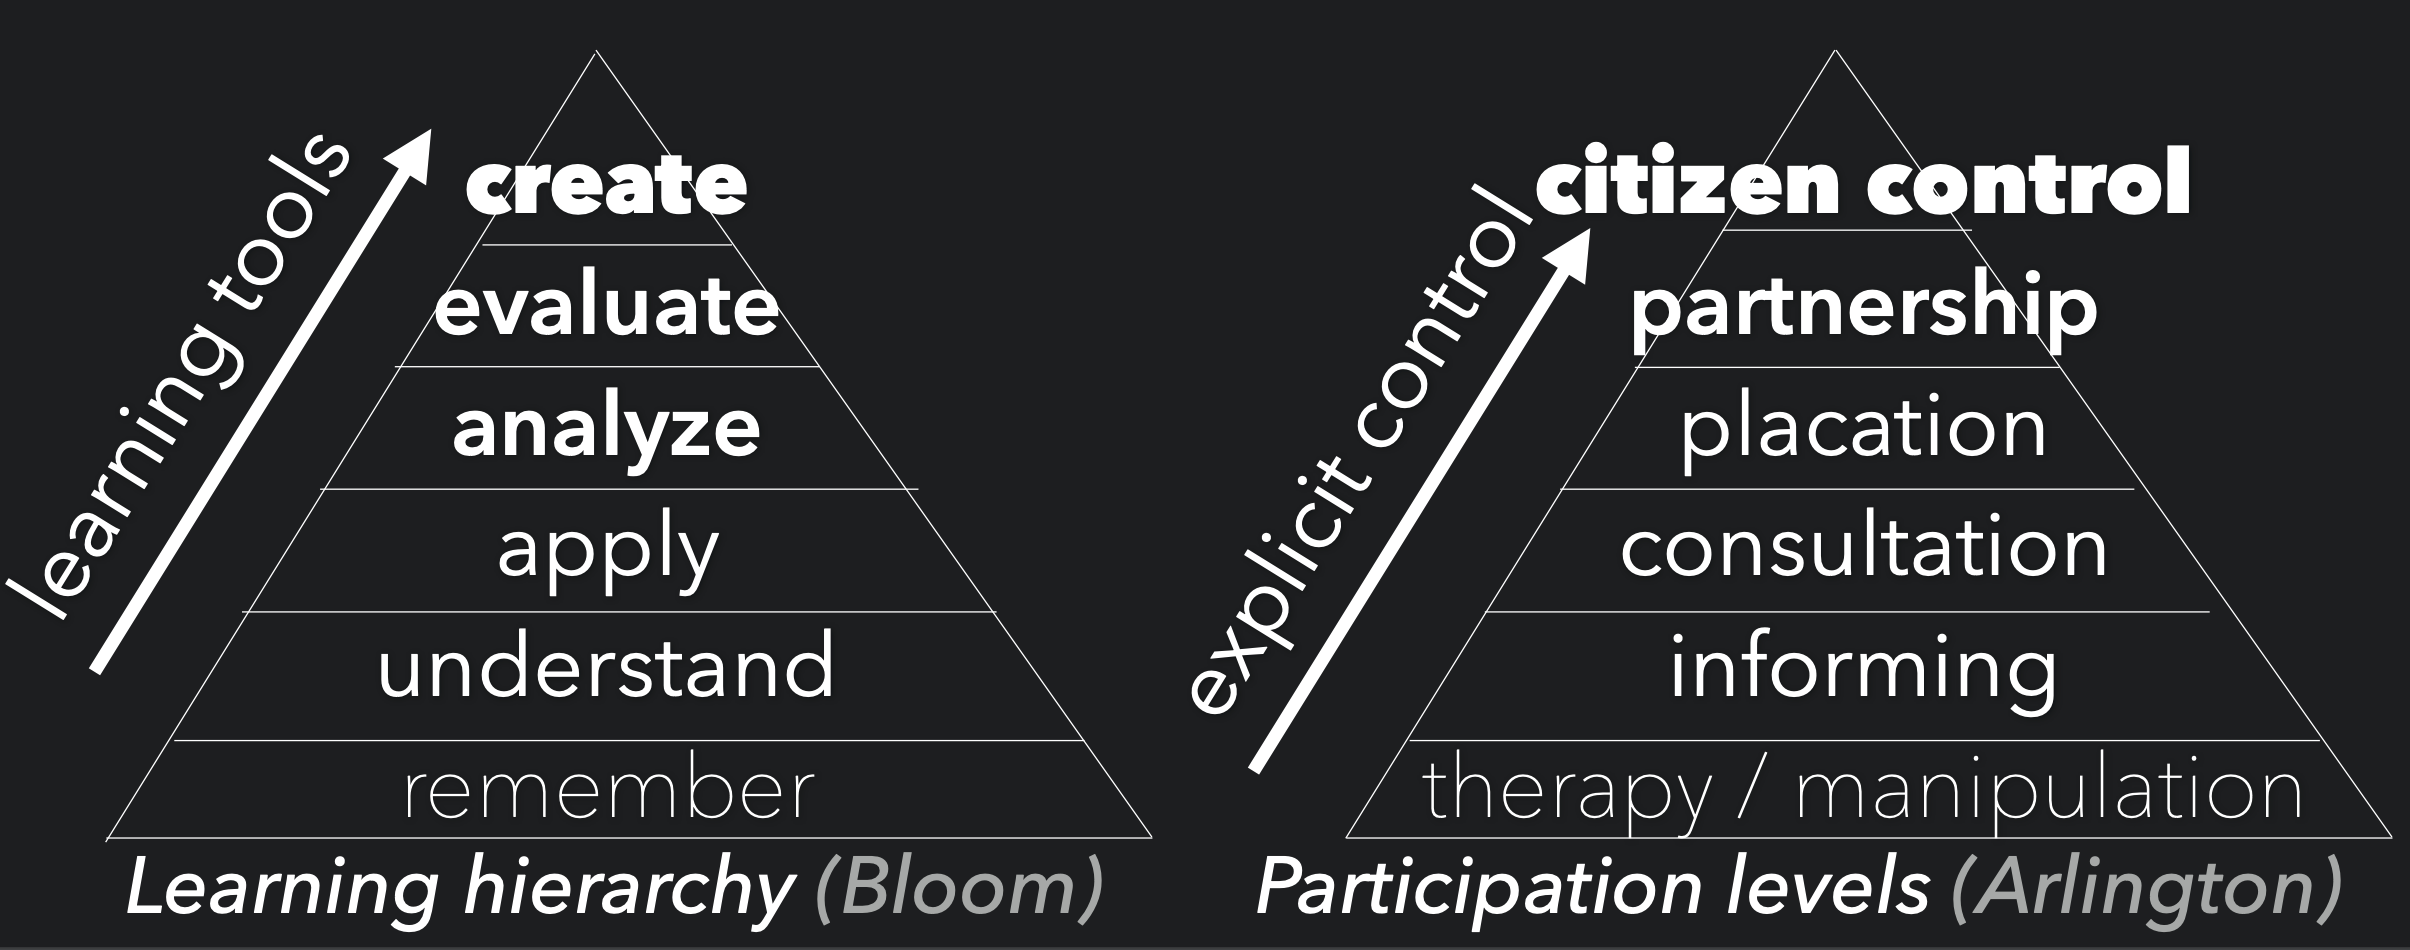
\includegraphics[width=1.0\textwidth]{figures/intro/intro-taxonomy}
  \caption[]
{Drawing from Maslow's hierarchy of learning and xx's hierarchy of contribution}
  \label{fig:intro-taxonomy}
\end{figure}

% come up with principles myself
%figure about conceptual and procedural learning 
\textit{Principles to integrate learning in social computing}: Learning broadly comprises conceptual (declarative) and procedural knowledge. Conceptual learning is where people learn what something is, learn about its features; this is a big part of current teaching. Typically, such learning is tested with test questions. In contrast, procedural learning teaches the {\it how} of things. How do you do x, y, or z.  Concpetual learning is useful when xxx while procedural learning is more useful when yyy.

To make useful contribution, people need to have a good working model of both the concepts and procedures for an activity. This dissertation enables this in two ways: 1) reifying conceptual bits in the software, and 2) providing procedural guidance with examples, checklists, and templates. Building on Maslow''s hierarchy~\ref{??}, it aims to push learning more up.

\textit{Principles to decompose Complex work to f(people, community, \& machines)}
% figure -- def needs one -- based on strengths and weaknesses
%fig - present a stack of things
The individual, groups of people, and machines possess complementary strengths. Individuals have personal motivation to do something; their lived experiences provide ideas that might be potentially novel. Groups of people might not be as motivated but might be willing to help by providing another set of eyes and complementary knowhow and insights from lived expeirences; they can help check biases with the diversity of their lived experiences. But since they are not as motivated, maybe limited affordances would be useful. Computers can implement things consistently to reduce biases but they cannot interpret open-ended instructions fairly in different contexts the way people can.  (todo- fix this to crisp english writing) (see slide deck)

Given these complementary strengths and limitations, this dissertation 1) begins every task with a heavy-handed implementation by an individual personally invested in that idea, 2) improves it with others'' feedback, and finally, 3) runs the idea with the help of automated software. For all these steps, the system manages the interdependencies beneath the sheets to reduce pressure on people. Building on xx's hierarchy~\ref{??}, it aims to push collaboration more up.

The efficacy of these techniques is borne out over multiple deployments. All these techniques have been put in systems as interfaces, intelligent backends, and so on... \\

%\begin{figure}[t!] 
%  \centering
%    \includegraphics[width=1.0\textwidth]{figures/img/intro/1-contributions}
%  \caption[Contributions of this dissertation]
%{Contributions of this dissertation including empirical results theoretical perspectives/techniques, real-world systems, and multiple outcomes}
%  \label{fig:contributions}
%\end{figure}

\subsection{User Interface and System Design}
%User interfaces and system design for efficient implementation
%figs needed to explicate 

While guidance techniques and role differentiation provide the building blocks, they are by themselves insufficient for useful higher-order collaborative work. These techniques need to be baked in simple, interactive interfaces. Multiple challenges show up for this question. First, the internet is a diverse community and have varying levels of expertise. So, the things need to be understandable to all. Second, people might have poor models of thiking about stuff and might frame their ideas and intuitions in weird ways.Third, the interface should make it easy to keep moving and get unstuck.  Too much information might make people struggle, so we need UIs for focused collaboration. 

This dissertation by bakes the techniques in the user interface  and by building a backend that is based on the principles of x, y, and z.

%System contributions
Gut Instinct  introduces a collaborative citizen science platform for people to transform lived exes into scientific theories. Gut Instinct frames the task of hypothesis-testing as a crowdsourcing problem, develops techniques and platform that supports different roles with just-in-time learning, and provides efficient backend support to automate simple tasks.

Gut Instinct divides multi-party collaboration into complementary tasks and supports them using different contribution mechanisms (like adding a question, editing a response) and roles (like experimenter, reviewer, participant). This provides people the flexibility to choose how much they’d like to contribute. Finally, Gut Instinct automatically manages multiple activities to reduce 
bias and experimenter/participant workload,such as randomized placement of 
people into conditions, maintaining anonymity, and collecting and cleaning data.


Take for instance, the state diagram — the edges represent what people need to do 
Roles Support via Just-in-time Skill Acquisition:  People take different roles--write up form galileo

%%"Furthermore, adding location information to photo collections is by itself insufficient for scenevisualization: we also need intuitive, interactive interfaces for exploring these scenes. There are several challenges faced in the design of such interfaces. First, unlike with Google Street View, where photos are taken at regular intervals, personal or Internet collections are typically an unstructured soup of photos. Nevertheless, the navigation controls should still be intuitive and exhibit regularity. Second, such controls should make it easy to find and explore the interesting parts of a scene, particularly for tourist sites."

%%%%%%%%%%%%%
\subsection{Outcomes}
\subsubsection{Empirical Results from Real-world Deployment}
expertise: limited; diversity: different countries; scale: some

\subsubsection{Dataset}
1. repo of hypotheses with rating
2. repo of experimental designs
3. ...

\subsubsection{Impact}
344 volunteers from 27 countries created 399 hypotheses about their health and the gut microbiome. Remarkably, microbiome scientists rated a fifth (75) of these hypotheses to have a scientifically valuable insight about a topic not covered by existing published work. Volunteers fleshed out 60 of these hypotheses into complete experimental designs. My entire work (code + data) is open source so others can edit, build, and experiment.

This dissertation has also enjoyed sufficient support in multiple research communities: Innovation researchers at MIT, online and offline fermentation and self-tracking communities, and citizen science groups. Finally, parts of the system have been taught in classrooms including CSCI 499: (Computing for Social Good) at USC. 

This work explores how online learning and process training systems, combined with
peer collaboration, can help people learn similar skills that
can be useful in scientific and design domains.


%%%%%%%%%%%%%%%%%%%%%%%%%%%%%%%%%%%%%%%%%%%
\section{Dissertation Roadmap}

%%%%%%%%%%%%%%%%%%%%%%%%%%%%%%%%%%%%%%%%%%%%%%%%%%%%%%%%%%%%%%%%%%
%todo- “we” refers to the set of authors…  -- see arvind

My dissertation demonstrates how we might draw on people’s diverse background knowledge, interest, and micro-expertise to expand scientific knowledge and push it in new directions. More specifically, the Gut Instinct platform that I have built instantiates these ideas enabling participants of the American Gut Project (the world’s largest crowdfunded citizen science project) to generate and experimentally investigate hypotheses (Figure 1). 

This dissertation creates the opportunity of harnessing humanity\textquotesingle s collective efforts to accomplish great goals.
s


"double quotes"


%The techniques make the idea concrete; the system operationalizes the techniques and makes them work; and the outcomes discuss the successes and failures of our approach.

%to people for them to perform personally meaningful work.
%My research prototypes collective systems for large-scale problems.
%Worldwide, people use online health fora to share insights and look for answers
%Iin short, to push people towards actively testing their ideas rather than just sharing them?  whether drinking kombucha really changes the gut constitution? In the absence of support and guidance, how can people do more? . 

%%1. novice-led
%    1. no experts
%    2. with other novices 
%2. personally meaningful 
%3. techniques
%    1. expert work to social computing 
%        1. ways to do that
%4. output
%    1. create new knowledge 

%   \chapter{Related Work}

\begin{quote}
\emph{This chapter summarizes research in citizen science, lead-user innovation, and social computing that inform the design of systems in this dissertation}. Citizen scientists have successfully solved expert-defined problems as sensors or algorithms. However, public involvement in scientific endeavors fail to provide a true participatory experience that is citizen-led and personally meaningful. Lead-user innovation provides a complementary setup. Lived experience, a tight feedback loop, and strong personal motivation enable people to create different and sometimes better products than experts; however, lead users rarely have access to training, conceptual knowledge, and pre-existing organizational structure for collaboration. Finally, social computing and crowdsourcing platforms support sharing potentially novel ideas but converting these to actionable plans requires expert guidance. This dissertation provides ways to integrate learning in social computing to enable deeper contributions from citizen scientists and lead users without expert involvement.
\end{quote}

%Professionals have the advantages of training, conceptual knowledge, and pre-existing organizational structure for collaboration and support; however, lead users rarely have access to such systematic support.

\begin{figure}[!h] 
  \centering
  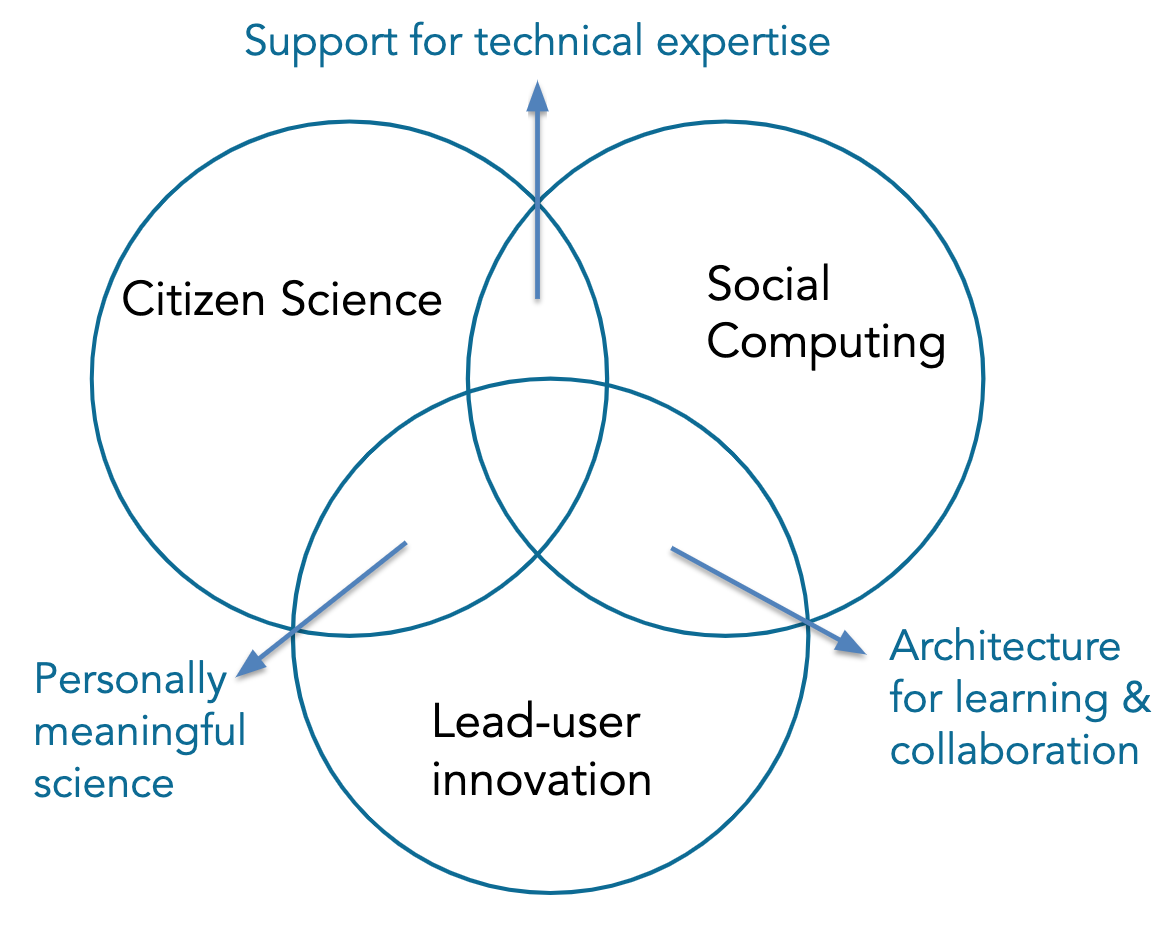
\includegraphics[width=0.6\textwidth]{figures/2-related/venn.png}
  \caption[]
{This dissertation draws from and contributes to citizen science, lead-user innovation, and social computing\index{related-1}}
  \label{fig:related-1}
\end{figure}

\vspace{0.25in}

%So, we find that there are three main challenges for citizen science: 1) make it personally meaningful, 2) deepen the contributions that citizens can make. 3. 1. Improve the quality of poor contributions — and improve the quality of max contributions     1. — hockey stick curve 
%%%%%%
\section{Science is increasingly networked but misses people’s lived experience }
Science is increasingly networked, multidisciplinary, and
open~\cite{Pandey2017}. For instance, \textit{LIGO}’s pathbreaking discovery of
gravitational waves brought together over 100 researchers
from over 100 institutions across 18 countries (ligo.org/about). 
Scientists increasingly share data and results faster (arxiv.org). 
Large scientific projects, like the \textit{Human Genome Project}, 
took to agile science by sharing methods, data, and insights to 
collaboratively speed discoveries. Scientists also form global 
collaborations to accelerate research in nascent scientific domains, 
like the Earth Microbiome project (earthmicrobiome.org).
At its best, institutional science has benefitted immensely
from large-scale global collaboration. Complementing this success,
many online projects enable people to help scientists~\cite{Nielsen2012}: annotating 
scientific papers~\cite{Good2013}; labeling galaxies~\cite{JordanRaddick2013}; and providing microbiome 
samples~\cite{McDonald2018}, CPU cycles (worldcommunitygrid.org), or personal data (openhumans.org). 
Efforts to further expand participation in scientific research are bearing fruit: \textit{Lab in the Wild} 
recruits anyone with an internet connection for behavioral studies~\cite{Reinecke2015}; and \textit{All of Us} aims 
to recruit one million Americans from all strata of society (allofus.nih.gov). Such collaborative efforts from experts 
and citizens suggest a new model for scientific work.

Often, when citizens participate in science, it is as \textit{embedded sensors} that 
are aggregated by experts. Public involvement in scientific endeavors continues
to be largely limited to performing tasks just beyond the reach of computers.
A classic example is \textit{Audubon}’s Christmas bird count, run since 1900
~\cite{Audubon2016}. Online examples include reporting flower blooms in
\textit{Project Budburst}~\cite{BoulderColorado2016}; recording wildlife activity~\cite{Faridani2009a};
identifying galaxies from satellite imagery in \textit{GalaxyZoo}~\cite{Zooniverse2007}; 
and biochemistry games: finding protein structures in \textit{Foldit}~\cite{Cooper2010}, 
synthesizing RNA molecules in \textit{EteRNA}~\cite{Lee2014}, and aligning 
nucleotide sequences in \textit{Phylo}~\cite{Kawrykow2012}. Distributed 
data contributions from people around the world—browsing online~\cite{Coviello2014}, using activity trackers, and joining scientific projects—have enabled valuable insights on topics including 
obesity~\cite{Althoff2017}, aesthetic preferences~\cite{Reinecke2014a}, sleep~\cite{F.lux2019}, and the human microbiome~\cite{McDonald2018a}. At their
best, these citizen science platforms yield novel insights.
For example, \textit{Foldit} players discovered protein structures
that helped scientists understand how the AIDS virus reproduces~\cite{Coren2011}. Why have such collaborative efforts succeeded?


%Different people provide different expertise that can vet claims and  fix mistakes~\cite{kane2009s}.
Collaboration benefits creativity when it brings different
 perspectives that build on each other; it impedes creativity (or worse, causes regression) 
when—through groupthink—it spreads biases rather than removing them~\cite{starbird2014rumors}. 
A humbling example of the power of fresh eyes: volunteer citizen scientists identified a new class of 
galaxies (\textit{green pea} galaxies) after researching green blots on \textit{Galaxy zoo} images; 
experts had dismissed these images as apparatus error~\cite{cardamone2009galaxy}.
This volunteer-led discovery demonstrates the need for fostering independent perspectives 
while simultaneously cultivating sufficient knowledge for meaningful domain contributions. 
Such collaboration requires strategic isolation: roviding just enough scaffolding to keep 
biases independent, while not stifling original ideas for bottom-up knowledge creation.

%This dissertation draws on the idea of people using  cognitive surplus to collaboratively answer scientific questions~\cite{Bonney2009}.


%%%% - where does this go
%Such bite-sized contributions is not without reason—a lot of
%scientific work requires deep conceptual knowledge and 
%training in scientific process to perform useful work. Most
%citizens lack the time, resources, and motivation to develop
%narrow, unique skillsets. Expanding the depth and breadth of work 
%performed by citizen science communities would be useful.

%\subsection{Citizen Scientists: From Collectors to Experimenters}
\subsection{Opportunity: Can people be scientists rather than just sensors?}
Citizens have successfully solved expert-defined problems as sensors or algorithms with a 
row-filling model of contribution.
In the quest to get people to track, measure, accumulate, or
sort both digital and analog data, citizen science has overlooked the massive 
opportunity of leveraging people’s unique advantages: our skills as reflective, 
creative thinkers who generate theories about the world, including ourselves.
People can offer more than just their data and perceptual
skills: they create theories, right or wrong, about a wide
range of topics including emotions~\cite{Johnson-Laird1992a}, motivation~\cite{Markus1991}, or
diet. These may be observational theories~\cite{Kempton1986}, folk theories
passed in a family/culture across generations~\cite{Gelman2011}, or ideas
brainstormed in online communities~\cite{23andme2016}. Perhaps, these intuitions 
can provide a starting point for independent, participatory experience that also assists the scientific community.

When are such personal experiences worth paying attention
to? For every intuition proven right, many more may be
closer to snake oil — e.g., the widespread belief in the utility
of probiotics despite limited evidence~\cite{Bonifait2009}. The global internet
increases the proliferation of both powerful and questionable
ideas: sharing speculation is fast while evaluation remains
slow. Moreover, people develop intuitions of cause and effect
that may or may not be correct. Current online forum
designs prioritize discussion — sharing personal details in
long, free-flowing text — over structure, succinctness, learning,
and potential scientific utility~\cite{Thomas2002}.

Advances in precision medicine have demonstrated the need
to engage people in uncovering and sharing insights~\cite{Aronson2015}. People
are highly motivated to improve their health outcomes,
more so if they suffer from a condition that severely affects
their quality of life, naturally forming communities. For example,
patients from the Amyotrophic Lateral Sclerosis
(ALS) community on \textit{Patients Like Me} (patientslikeme.com)
organized a study to track effects of Lithium on their symptoms
~\cite{Wicks2011}. This is not surprising; lead users excel at tackling
\textit{need-intensive} problems where they can use their lived
experiences to identify problems, try solutions, and readily
observe the effects~\cite{VonHippel2005}. Other organized communities like
\textit{Quantified Self} hope to uncover lifestyle patterns that may
improve their productivity and health outcomes. The word
‘self’ belies the fact that such movements are highly collaborative:
amateurs frequently share experiences and invite
feedback on online fora (patientslikeme.com) and blogs
(ibsgroup.org). Millions follow these ideas and some incorporate
these intuitions in their lives. What kinds of scaffolds
and structure may help people generate better ideas and implement them as actionable plans that
enable researchers to identify promising insights?

%How can people expand their insights into scientific work?

Most scientists develop their skills through an apprenticeship-
based graduate school experience. Apprenticeships emphasize
hands-on experience with individualized, taskspecific
feedback~\cite{schon1984reflective}. Scientists possess a wealth of declarative
knowledge about their domains (e.g., how to set up a
randomized controlled trial), and also procedural knowledge
—some narrow, some broad —towards getting things done
(e.g., improving fMRI signal intensity by having participants
consume cocoa beforehand~\cite{Francis2006}). This dissertation explores how
online learning and process training systems, combined with
peer collaboration, can help people learn similar skills that
can be useful in scientific domains.
%So, we find that there are three main challenges for citizen science: 1) make it personally meaningful, 2) deepen the contributions that citizens can make. 3. 1. Improve the quality of poor contributions — and improve the quality of max contributions     1. — hockey stick curve 
%WOULDN'T IT BE GREAT TO HAVE PEOPLE DESIGN AND RUN EXPERIMENTS AS AN INSTANCE OF COMPLEX SCIENTIFIC WORK
%Link to lead users -- people already doing personally meaningful work.. 

%%%%%%%%%%%%%%%%%%
\section{Lead users Succeed When They Know What to Do and How to Do It}
%“Lead users are rarely experts by themselves. They are novices who find themselves at the right place, with the right tools (that they might have created themselves), and who have the courage to follow through.” Lead users have created different—and in some cases better designs— than experts. 

%examples: UN example (see eric vh)

Lead-user innovation is both an inspiration and an application area for this dissertation. Lead users are
users of a product (or service) who experience advanced needs unmet by existing products~\cite{VonHippel2005}. The
power of lead-user innovation is that lived experience, a tight feedback loop, and strong personal
motivation can yield different and sometimes better products than experts [32]. For example, diabetes
patients have improved insulin delivery [47] and snowboarders have improved their binding
ergonomics. Lead users also collaborate online to build software
(github.com), create novel hardware \& reference designs
(openaps.org), and share personal data (quantifiedself.com,
openhumans.org). Some go further still, e.g., the transcranial
direct-current stimulation community draws ideas from scientific
papers to attempt self-experiments (reddit.com/r/tDCS). In a few exceptional cases, lead users have authored
scientific papers, e.g., Open Artificial Pancreas creator
Dana Lewis discussed the benefits and challenges of first-generation
automated insulin delivery at the 2016 American
Diabetes Conference~\cite{DanaLewis}.

Why do people do this? Curiosity, personal learning, and social
comparison are three reasons~\cite{Reinecke2015}. A massive interest in
personal genomics (over 1 million 23andme participants)
and the human microbiome (13,000 \textit{American
Gut} participants) demonstrates people’s yearning for self-understanding.
Users of these platforms send data, answer survey questions,
and discuss on fora. Some even use online lectures to understand
concepts of genes, phenotypes, and microbiota~\cite{23andMe2017, Knight2016}. 

\subsection{Opportunity: Providing lead users the expertise to tackle complex knowledge work}
Sometimes, having a different background
 than experts can be beneficial. Shared knowledge is great when it’s right, but blocks progress
 when wrong. When false assumptions limit experts, at least some novices are likely to be 
\textit{uninfected}. The converse also holds, and much more often: novices are also uninfected
by all the knowledge that enables experts to innovate. Lead users have an advantage when the key ingredient is experience intensive; experts retain the
advantage for \textit{solution-intensive} innovations [32]. In a large distributed community, 
there’s often someone who happens to have important relevant knowledge, usually 
drawing on a relevant but distant domain. Having many people work on the same problem 
increases the odds that one will break through. Drawing on secondary expertise as 
inspiration can be an important agent of creativity because almost by definition, the
 combination is rare~\cite{Boden2004}. 
%For example, GalaxyZoo volunteers discovered ‘green pea’ galaxies overlooked by scientists who mistakenly assumed the green hue was merely an imaging artifact~\cite{Tinati2015}. 

Community-driven approaches to understand personal
health and well-being largely reside outside the realm
of institutional science and medicine. While some fads and beliefs are 
questionable at best, on occasion communities
break new ground that may provide widespread value,
such as fecal transplants to alleviate \textit{Clostridium difficile} infection
symptoms~\cite{Brandt2012}. Some doctors recommend that patients
track their symptoms and reflect upon them to find
insights. Putting people in charge can help them find significant
relief for ailments like chronic migraine~\cite{Gawande2017} and provide
researchers and clinicians with useful patient data
(smartpatients.com). Insights from N\Hair=\Hair1 studies have helped
crack scientific puzzles about the working of the mind~\cite{V.S.Ramachandran1998},
heart, and microbes~\cite{Weisse2012}. 

Personal needs and challenges can be highly motivating but performing complex work still requires multiple rounds of trial and error. 
People need to know the genre of work and implement it correctly.  Professionals have the advantages of training, conceptual knowledge, 
pre-existing organizational structure for 
collaboration and support, and direct access to resources. Lead users either seek these resources from others or need to create them. 
Providing a correct and complete model for complex, structured activities might reduce efforts and improve the quality of results.
This dissertation reduces the gap between lead users' ideas and implementation by providing templates for 
genre work using just-in-time training and a collaboration platform to find others. This dissertation focuses on enabling people transform their idea to a controlled experiment as opposed to 
self-tracking or informal iteration which is the focus of most current citizen-led work in health.

\subsection {Case: Scientific experimentation is difficult}
While public contributions have supported institutional science; it’s rare for citizens to design
their own experiments. A number of health and behavioral research projects enlist citizens as helpers (e.g., \textit{HabitLab} [43]). 
\textit{CivilServant} enables online communities’ 
moderators to test policy ideas; moderators share these ideas with researchers who transform 
them to study designs [51]. Through the \textit{PatientsLikeMe} website (patientslikeme.com), citizens 
and scientists created a study investigating whether consuming lithium alleviated ALS symptoms [64]. 
While an initial scientific study had provided positive benefits, both this citizen science study and 
a subsequent university study did not find benefits. \textit{Tummy Trials} asked 
participants to generate health questions, introducing a protocol for self-experimentation 
combining ideation and self-tracking [36]. In all these cases, citizens rely on experts to provide sound experimental design.

Why is experimentation hard?  Despite a predetermined goal and a formalized process, experimentation
requires making situationally-appropriate decisions. A dependent variable may produce crisp
numbers but feedback on the experiment design itself is more multifarious. Good experiment
design is inherently user centered: how will participants interpret the instructions? Experiment
designers need awareness of others’ interpretation of their ideas and asks. Feedback and iteration
might be key to creative success, especially for novices. Providing feedback on experiment
designs requires knowing the success criteria and how to
help improve.  Feedback can be provided by experts~\cite{dow2012shepherding, schon1984reflective}, peers~\cite{Boud1995, Kulkarni2015b}, software~\cite{Dantoni2015, Head2017}, or even oneself~\cite{Boud1995,schon1984reflective}. While feedback from novices can
potentially improve both structure and content, it can also emphasize superficial issues over the
underlying structure~\cite{chi1981expertise}. Finally, successfully running an experiment
requires managing multiple processes such as random
assignment, anonymizing participant details, and sending
instructions and reminders for data collection.

%%%%%%%%%%%%%%%%%%%%%%%%%%%%%%%%%%%%%%%%%%%%%%%%%%%%%%%%%%%%%%%%%%%%
%But to understand that let's look at social computing ideas...

\section{Social Computing and Crowdsourcing Architectures for Complex Work}
Canonical crowdsourcing breaks larger tasks into microtasks; algorithms specify the division,
dependency, and agglomeration activities while workers perform small tasks supported by task-specific
guidelines~\cite{kittur2012future}. Leveraging existing expertise is one approach for complex knowledge work. One strategy
directly employs experts’ just-in-time feedback to improve crowd work~\cite{dow2012shepherding}. Workflows manage
experts for open-ended work like developing interactive prototypes~\cite{Retelny2014}. 
\textit{Flash Organizations} uses automated hiring, a hierarchy with a central leader, and optional 
team leaders for collaborative projects like product design~\cite{Valentine2017}.
Another strategy creates roles that enable more experienced crowd members to orchestrate
the work. \textit{Ensemble} supports leaders in guiding and constraining crowd 
contributions~\cite{Kim2014e}. Role-based approaches confer three benefits: 1) clean 
delineation of responsibilities improves chances of task completion, 2) clustering similar tasks 
reduces overhead and increases consistency; 3) people can decide their contribution levels. 
However, experts are expensive, in short supply, and sometimes prone to groupthink. 

Carefully-constructed interfaces can aid novices with task-specific expertise to solve problems 
that only experts previously could. \textit{Foldit} introduced 3D game for specifying low-energy protein 
structures via direct manipulation~\cite{Cooper2010}. Making a challenge visually salient is an 
effective way to on-board novices. For tasks that don’t have as a crisp visual analogue as protein
folding, people need better conceptual support. Prior work has explored collaborative hypothesis generation and testing on pre-existing data sets
~\cite{luther2009pathfinder,willett2011commentspace}. This dissertation offers a 
complementary contribution: enabling citizens to generate data on topics of personal interest.

One way to make complex tasks manageable is to divide them into distinct phases. 
Touchstone demonstrates the power of a semi-automated workflow integrating experiment 
design, testing, and analysis~\cite{Mackay2007}. Crowdsourcing has similarly innovated by 
creating distinct phases: break larger tasks into microtasks; algorithms specify the division, 
dependency, and agglomeration activities while workers perform small tasks supported by 
task-specific guidelines~\cite{lasecki2012real}. From these systems, our work draws the 
idea of dividing experimentation into multiple tasks—some self-sourced, others 
crowd-sourced; and introduce just-in-time domain expertise to perform these tasks. 

 
%How might groups of novices perform complex work like experimentation?
%Systems like Foldit and EteRNA powerfully show  how carefully-constructed interfaces provide
%novices with the task-specific expertise to solve problems that only experts previously 
%could~\cite{Cooper2010, Lasecki2012, Lee2014, Zooniverse2007}.

%%%%%%%
%%building up solution space - more work
\subsection{Learning resources at the right time}
Providing just-in-time supports, step-by-step instruction, and showing helpful supportive
 information are core ideas in instructional design~\cite{Kirschner2008}. Crowdsourcing 
systems leverage interactive guidance for specific tasks. For example, \textit{CrowdLayout} and 
\textit{Cicero} provide guidelines and static rules that workers use these to reason about their choices
 and improve network layouts~\cite{chen2019cicero, Singh:2018:CCD:3173574.3173806}. 
Others like \textit{CrowdSCIM} and \textit{Crowdclass} scaffold pre-task interventions~\cite{Lee2016,wang2018exploring}. 
While learning resources are distributed across the internet, they are rarely integrated with the task. 

Creative, open-ended work has rich pedagogical value. Online work, like 
online learning, requires appropriate scaffoldings, such as rubrics
~\cite{Boud1995, Kulkarni2013peer}, decision trees~\cite{Lee2016,Yu2006}, 
tutorials~\cite{Andersen2012}, and quick expert guidance~\cite{dow2012shepherding}. 
Similar to general critique of pure discovery learning~\cite{Mayer2004}, simply 
asking participants to \textit{figure it out} would be poor pedagogy. Hence, this dissertation
introduces a guided discovery learning approach as Mayer advocates: expert-curated 
learning materials help participants start, with discovery following. Such integration 
offers a problem-based learning experience with context and 
motivation for the material students learn~\cite{Savery1995}. In principle, these 
real-world problems also provide a yardstick for measuring learning. 

This dissertation introduces support during the task itself for those with little-to-no mental model of the knowledge domain. 
Like the \textit{Shepherd} review-writing system~\cite{dow2012shepherding}, this dissertation provides just-in-time support. 
There are two key differences: 1) this work scaffolds the entire creation process, not just the post-draft feedback
 stage, and 2) it does not draw on expert time – the knowledge is implemented in the software itself. 
%todo-repeated too many times


%%%%%%%%%%%
\section{Microbiome research: a petri dish for personally meaningful scientific work}
The human microbiome is the collection of all microbes and
their genetic components in and on our bodies. It is highly
personal: each of us hosts a different collection of microbes,
and this collection is influenced by our environment, diet,
health, lifestyle, and genetics. A major scientific effort is to
better characterize and understand this diversity and the
causal factors for it (hmpdacc.org). Understanding the human microbiome requires insights
into people’s lifestyles. Microbiome science is nascent, highly contextual, and personally motivating.
However, research has only scratched the surface of understanding the microbiome and using it 
to improve our wellbeing. Engaging diverse participants at scale can potentially yield exciting new results.


The \textit{American Gut Project} (americangut.org) offers a
crowdsourced opportunity for people to get a microbiome
sampling kit~\cite{KnightLab2016a}. AGP
participants contribute their samples for bacterial marker
gene sequencing and analysis~\cite{Debelius2016}. Participants then receive
a summary of their results with all their raw data. Anonymized data is publically available.

To date, more than 13,000 people have participated.
Participants submit both a physical sample and fill out
a survey. AGP seeks to build a comprehensive map of the human microbiome, and identify
its healthy and unhealthy components. Analysis has revealed lifestyle-microbiome correlations
of dog ownership and beer or vegetable consumption,
among others.

\subsubsection{People hold the key to understanding the gut microbiome}
The structure of the human microbiome is influenced by many factors, including age, genetics, diet, and xenobiotic and antibiotic use~\cite{Gill2006}. The gut microbiome in particular plays an important role in metabolism and immune system development, and some microbiome dysbioses have been associated with diseases such as obesity, inflammatory bowel disease, type I and type II diabetes, autism, multiple sclerosis, and malnutrition~\cite{Cho2012}. The human microbiome is impossible to understand without information about its host~\cite{Debelius2016} and many influence factors remain unknown. Teaching people about the gut microbiome and having them guess associations between the microbiome and health and disease states can potentially accelerate the process of discovering links between diet, disease, and lifestyle factors and the gut microbiome.

Currently, the topics for scientific investigation are handpicked
by a small group of scientists. Can opening up the
scientific process to the world yield additional insights?
How can people’s situated knowledge supplement institutional
science? This dissertation provides systems and techniques for novices to complement experts in creating new knowledge about the microbiome. \\

%Crowd workers perform better when they understand their efforts’ importance. For example, Mechanical Turk workers analyzing radiology images performed better when told of the medical purpose: finding cancerous tumors~\cite{Chandler2013}. Motivation can also be personal. For example, 23andMe is a genetic testing site and online service that includes a discussion board. On this forum, a user reported disliking the sounds of others eating. She’s not alone; a 23andMe survey found 16,000 users with the same condition and a predictive genetic similarity among them~\cite{23andMe2016}.

This chapter provided an overview of related research; chapters dedicated to specific systems discuss additional research that informs that design of those systems. This dissertation explores integrating learning in social computing for complex, creative work with two goals in mind: efficacy of the resulting systems (i.e. usability, correctness, and existential evidence) and generality of the underlying techniques upon which the tools are built.
%
% Of course, if you prefer, you can just start with
%   \chapter{My First Chapter Name}
% and start typing away.  

\begin{comment}
\chapter{Just a Test}
This is only a test.
\section{A section}
Lorem ipsum dolor sit amet, consectetuer adipiscing elit. Nulla odio
sem, bibendum ut, aliquam ac, facilisis id, tellus. Nam posuere pede
sit amet ipsum. Etiam dolor. In sodales eros quis pede.  Quisque sed
nulla et ligula vulputate lacinia. In venenatis, ligula id semper
feugiat, ligula odio adipiscing libero, eget mollis nunc erat id orci.
Nullam ante dolor, rutrum eget, vestibulum euismod, pulvinar at, nibh.
In sapien. Quisque ut arcu. Suspendisse potenti. Cras consequat cursus
nulla.

\subsection{A Figure Example}
\label{ssec:figure_example}

This subsection shows a sample figure.

\begin{figure}[h] 
  \centering
  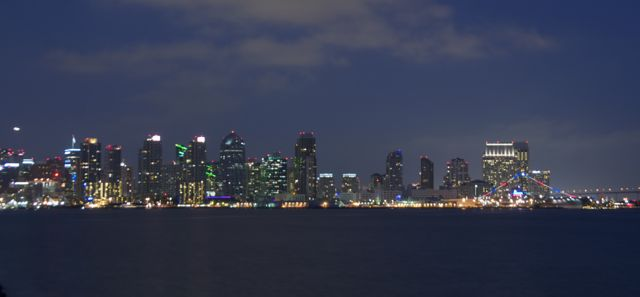
\includegraphics[width=1.0\textwidth]{sandiego}
  \caption[A picture of San Diego. Short figure caption must be \protect{$< 4$} lines in the list of figures]
{A picture of San Diego.  Short figure caption must be \protect{$< 4$} lines in the list of figures and match the start of the main figure caption verbatim. Note that figures must be on their own line (no neighboring text) and captions must be single-spaced and appear \protect\textit{below} the figure.  Captions can be as long as you want, but if they are longer than 4 lines in the list of figures, you must provide a short figure caption.\index{SanDiego}}
  \label{fig:sandiego}
\end{figure}


%%%% TABLE 1 %%%%
\vspace{0.25in}
\begin{table}[!ht]
\caption[A table of when I get hungry.  Short table caption must be \protect{$< 4$} lines in the list of tables]{A table of when I get hungry. Short table caption must be \protect{$< 4$} lines in the list of tables and match the start of the main table caption verbatim.  Note that tables must be on their own line (no neighboring text) and captions must be single-spaced and appear \protect\textit{above} the table.  Captions can be as long as you want, but if they are longer than 4 lines in the list of figures, you must provide a short figure caption.}

\vspace{-0.25in}
\begin{center}
\begin{tabular}{|p{1in}|p{2in}|p{3in}|}

\hline
Time of day & Hunger Level & Preferred Food \\

\hline
8am & high & IHOP (French Toast) \\

\hline
noon & medium & Croutons (Tomato Basil Soup \& Granny Smith Chicken Salad) \\

\hline
5pm & high & Bombay Coast (Saag Paneer) or Hi Thai (Pad See Ew) \\

\hlinet
8pm & medium & Yogurt World (froyo!) \\

\hline
\end{tabular}
\end{center}
\label{tab:analysis3}
\end{table}

\end{comment}


%%%%%%%%%%%%%%%%%%%%%%%%%%%%%%%%%%%%%%%%%%%%%%%
%\chapter{Scaffolding Citizen-led Complex Knowledge Work}
\chapter{Social Computing for Complex Knowledge Work}

\begin{quote}
\emph{This dissertation explores how the following things happen. Complex work is hard. Needs learning. People do things in groups. Social computing misses learning (learning is around but not here). why your title is what it is, what that means, how you set up your arguments, and what claims your introductory chapter makes. Current online platforms (like Facebook) are built on insights from psychology about capturing people’s attention. My research instead takes a more socially responsible approach by integrating learning theory and collaboration for people to perform complex work such as generating and evaluating scientific theories. This has the potential to diversify the stakeholders and contributors to our future society.}
\end{quote}
\vspace{0.25in}

Social computing platforms have revolutionized how most people connect, communicate, and share. We increasingly connect with friends and strangers in different ways for a number of purposes. Friends and family can stay in constant touch with their loved ones. Strangers from different parts of the world discuss their ideas about their health. Increasingly, these connection opportunities have also translated to more active doing: people fund other's\'  ideas that traditional business places might balk at. Some have used social platforms to amplify their voice and bring about social changes. for instance, people in Sudan have taken down dictators [??]. By transforming how we communicate, share, and chat, social computing has become perhaps the greatest internet-fueled change of our times. 

%%interactive vis (social computing discussions) is awesome
% people can do stuff with hypotheses (test them?)
%    however, viz is hard (scientific work)
%        programming toolkits needed and impose burden (support needed to get started, reduce burden, and …)

However, the benefits of social computing are not distributed equally. While everyone has a voice, some have bigger loudspeakers than others: xx\% of most popular posts are from experts. While anyone can organize and bring changes, collective attempts to organize frequently fail. While anyone can learn from widely accessible research papers and articles, people create faulty insights from self-tracking and conspiracy theories abound. With this lens, social computing seems less transformative but rather a highly scaled up version of the offline reality of limited expertise people live in. 
% 1 to 1 link with the first para

%\subsection{Pivot to people - People can do great things but need help...}
%Well, what are people good at? What are they motivated to do? 

%People have complementary knowledge in comparison to experts and are uninfected by expert biases; these insights are drawn from lived experience, both individual and collective.

Specific to this dissertation: While social computing platforms have vastly succeeded at keeping people engaged and sharing, they barely support \textit {citizen-led enquiry}. People have strong personal motivations and contextual insights. People possess a remarkable ability to identify patterns and create theories from their experiences [??]. While most people have an amazing breadth and depth of ideas, they lack the expertise to implement these ideas. To create knowledge, they need mental scaffolds for organizing complex work, domain knowledge to compose and execute the steps, and ways to ask for help. Experts benefit from conceptual knowledge, professional training, pre-existing organizational structure for collaboration, and direct access to resources. Currently, citizens lack these resources. social computing platforms where people spend ridiculous times provide little support. 

%this is the current state --  this is the big challenge, why is it a challenge
%% however, scaling good teaching is hard - kulkarni
%     this peer thing can be helpful (evidence from small studies)
%        however, this is challenging — 2 causes
%        interfaces need to provide scaffolding 


\begin{figure}[b] 
  \centering
  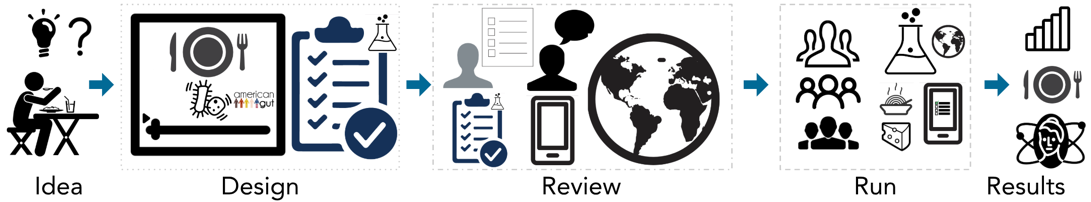
\includegraphics[width=1.0\textwidth]{figures/intro/intro-1}
  \caption[]
{The Gut Instinct platform enables anyone to transform their intuitions to hypotheses 
and then design and run experiments to test them [xx-xx]. Gut Instinct integrates 
conceptual learning embedded via short lectures and software-guided procedural 
learning to enable designing and reviewing experiments. Participants from around
 the world join experiments, follow instructions, and pro-vide data in response to 
automated data collection reminders. }
  \label{fig:intro-1}
\end{figure}

Consequently, this is unfortunate missed opportunity for both individuals and the world at large. Enabling peoplt to learn to perform personally meanignful work can help them answer their own questions. People's ideas can catalyze creating new knowledge that we are missing out on.  How might online systems support citizen-led knowledge work? 

Let''s reflect on this dual nature:  science can answer life-relevant questions but few know how to even get started. As a result, people fail to answer their questions and institutional science misses out on ideas from beyond the ivory tower. 

%one line to summarize my work -- see other intro

%two properties of classes help us - kulkarni
%this thesis leverages these two properties and provides a new class of benefits etc... 

%what helps us
%1. the scientific method is structured
%    1. even though creative and open-ended
%2. roles: people take them online
%    1. captures diversity — breadth
%    2. micro-expertise supports this explicitly 
%3. procedural learning: can teach people how to do things
%    1. captures learning — depth


This dissertation advances the design of social computing systems by integrating learning and collaboration to enable complex work such as generating and evaluating scientific theories. Over 600 people from 30 countries have self-organized to generate theories about the human microbiome and test them by running experiments. This dissertation raises the question: how can global communities create knowledge that meets their goals without waiting for experts to lead? 

Gut Instinct emodies this insight and introduces a collaborative citizen science platform for people to transform lived exes into scientific theories. 

%%%%%%%%%%%%%%%%%%%%%%%%%%%%%%
\section {People already do great things but struggle with complex tasks}

\subsection{People are awesome}
People design, build, and track to better understand and improve their health [?? dana lewis].  On numerous online fora, people share their intuitions, observations, folk theories, and even results from trying different approaches to improve their health, e.g. from simple ideas like ‘giving up drinking coffee to improve quality of sleep’ to tests and dietary approaches. People draw ideas from current research by reading and discussing papers. In many cases, these discussions are not just anecdotal but also derive from state-of-the-art scientific work. In some cases, people contribute back to scientific work as well.How can social computing platforms effectively enable people to do more personally meaningful work built upon their experiences and insights?

People’s curiosity, needs, and possibilities to do useful work is endless; however, traditional online systems don’t support them. Online fora encourage long, rambling discussions. Online learning provides conceptual lessons but people drop out and these are not linked to people’s needs.While learning resources like MOOCs abound, they hardly meet the need: many drop out, the lectures focus on conceptual knowledge, and lack the feedback needed to perform open-ended creative work. We know little about integrating learning resources and social computing affordances are far from each other. Moreover, currently both learning and work are not personal; can we change this? Lack of appropriate "learning abstractions" make complex work unrealistic.

The goal is to create environments for learning and collaboration through complex, personally meaningful work.

%%%%%%%%%%%%%%%%%%%%%%%%%%%%%%%%%%%%%%%%%%%%%%%%%%%
\subsection{Challenge: People' don't know what to do and how to do it}
Citizens have a different background than professional scientists; they have unique
 personal experiences but lack the years of domain training. Two major issues in 
enabling complex work on the internet are (diversity and scale?) 
quality of individual contribution and managing overall contributions from the crowd.
We desire social computing techniques that reliably enable a wide variety of people to 
contribute more than they naturally could and that manage the dependencies among
 a large set of tasks.

To create computational systems that leverage their strengths and mitigate the lack of training, this dissertation 
focuses on domains where the science is nascent, highly contextual, and personally motivating.
 Synthesizing the crowdsourcing literature and my experience highlights three challenges: 
poor signal-to-noise from crowds due to lack of training; inefficient collaboration without 
careful attention; and poor results (or no results at all) unless experts lead. 

To address  these concerns,  this dissertation introduces and evaluates peer production architectures 
and procedural learning.

\subsection{Scientific experimentation: An instance of complex knowledge work}
%here''s an example: experimentation 
Supporting complex knowledge work has been a challenge for Human Computer Interaction
 research (make specific). For instance, many people are interested in understanding and 
improving their health. Millions of peple from all over the world share their insights. 
Can't they run experiments for these?

Scientific experimentation features technical requirements and contextual choices 
that are inscrutable for a lay individual yet necessary for success [??]. While 
professional scientists and commercial ventures run experiments every day, with 
notable exceptions [??], empirical papers from non-professionals are 
vanishingly rare. This biases the questions asked, studies run, and knowledge 
created [??]. People have questions about their health, but lack the expertise 
and resources to scientifically investigate them. Broadening the pool of 
experimenters could help people investigate their curiosities, develop solutions 
to improve health and performance, and assist institutional researchers.


\textit{People lack the expertise to know what to do and how to do it.}. 
Success with complex creative activities requires procedural
knowledge (how to do things) in addition to conceptual
knowledge (facts). While many resources offer facts, procedural
learning is often ignored.The converse also holds, and much more often: novices are also
“uninfected” by all the knowledge that enables experts to
innovate.Sometimes, having a different background than experts can
be beneficial. Shared knowledge is great when it’s right, but
blocks progress when wrong. When false assumptions limit
experts, at least some novices are likely to be “uninfected”.
For example, GalaxyZoo volunteers discovered ‘green pea’
galaxies overlooked by scientists who mistakenly assumed
the green hue was merely an imaging artifact [54]. 


% kulkarni -- "This assessment requires bothcommon-sense knowledge to understand student work and the expertise to assess tacit criteria such as “well-designed” or “well-modularized” that cannot be completely articulated. Indeed, teaching such tacit criteria is an important goal in open-ended domains like design"


\textit{People lack a professional network to improve their work}. 
Furthermore,  how do people ask others for help? Who do they reach out to?

People are connected online and collectively have access to many resources.
In a large distributed community, there’s often someone who happens to 
have important relevant knowledge, usually drawing on a relevant but 
distant domain. Such distributed efforts are a type of lead-user innovation [31]. 
Having many people work on the same problem increases the odds that 
one will break through. Drawing on secondary expertise as inspiration can
 be an important agent of creativity because almost by definition, the 
combination is rare [10]. %Open \& crowd innovation builds up on contributions
 by diverse online participants, and a ‘bubbling up’ process for strong ideas [56].

While many hands make light work, novices need clear contribution opportunities. 
The crowdsourcing literature offers many good verification approaches for tasks 
with clear right or wrong answers – like whether two images represent the same 
product or what street number is written on a sign. However, verifying knowledge
 work necessitates a different approach because it requires making 
situationally-appropriate choices. 

%%%%%%%%%%%%%%%%%%%%%%%%%%%%%%%%%%%%%%%%%%%%%%%
\section{Thesis Statement and Contributions}
\noindent This dissertation investigates the question: how to enable people to perform personally meaningful work otherwise beyond their expertise? Underlying these investigations is the thesis:
%"My thesis statement is"
\begin{quote}
\emph{Providing task-specific guidance in social computing enables personally meaningful \& useful scientific work}
\end{quote}

This dissertation\textquotesingle s primary contribution is the idea of intergrating learning in social computing to enable groups of novices to perform complex, creative activities. The thesis achieves this integration by building a sequence of interactive prototypes that enable people to collaboratively generate and test hypotheses. In the process, the prototypes divide complex work into distinct activities: self-sourcing the design and crowdsourcing people''s inputs and data. Every prototype advances social computing further as a domain for deep, personally meaningful work. Beyond introducing learning abstractions, this dissertation carefully designs the affordances, support, and system to enable different users for different needs. 

 %To realize this idea, 
This dissertation makes three types of contributions: theoretical perspectives/techniques, real-world systems, and outcomes including empirical results, systems lessons, and dataset (Figure \ref{fig:contributions}). 

%%%%%%%%%
\subsection{Theoretical  Techniques}
Improving  work quality in social computing suggests deepening individual contributions and broadening participation by providing different contribution mechanisms.The former requires better learning tools and the latter requires better collaboration tools and dependency management. Consequently, this thesis' theoretical contributions include 1) principles to integrate guidance for complex tasks, and 2) ways to divide complex tasks into multiple roles or affordances.

%“..adapts and extends techniques from xxx” -  arvind

%system-led learning vs people-led
Traditional systems think of knowledge as being provided by the people, while we being the knowledge from the system itself.

%todo-introduce the learning and collaboraiton taxonomy here
\begin{figure}[b] 
  \centering
%  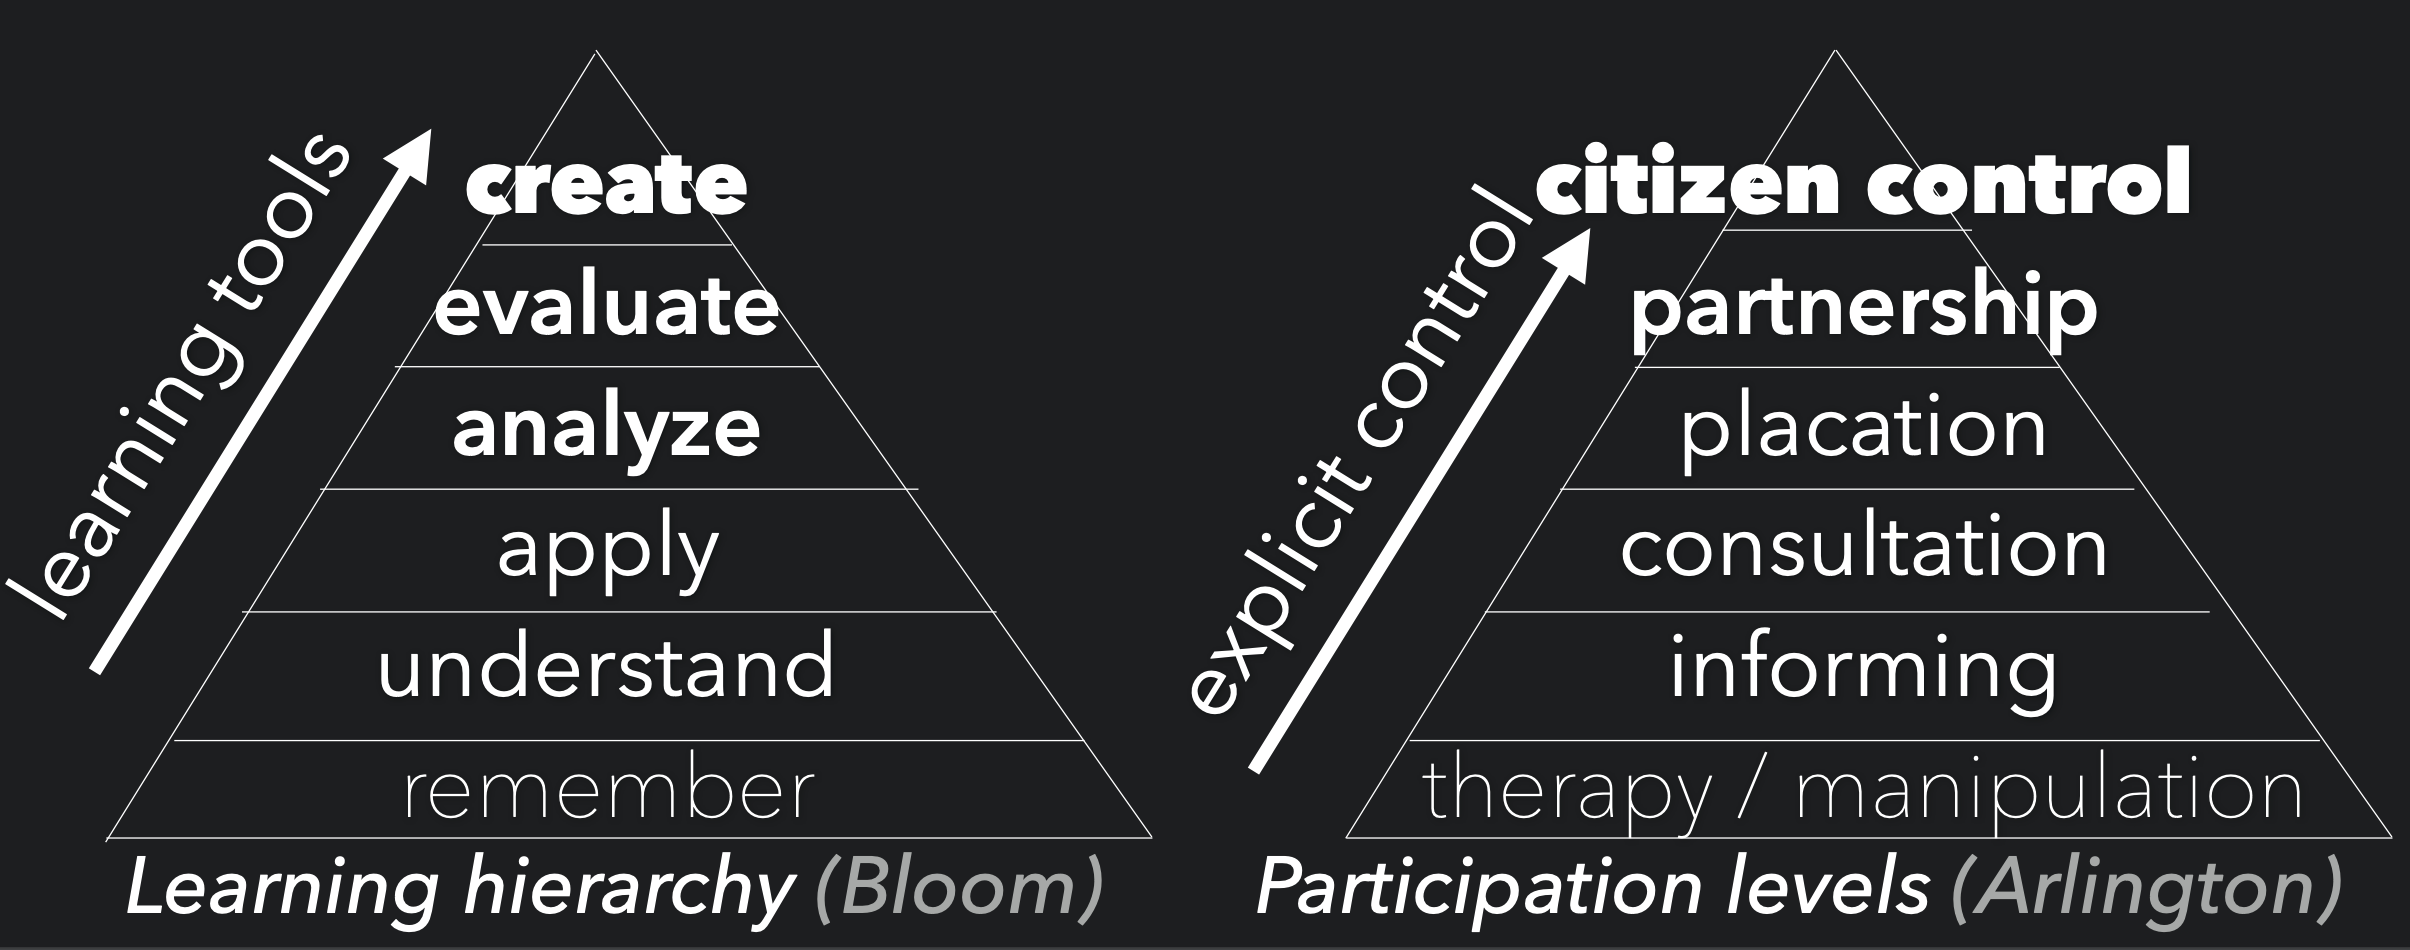
\includegraphics[width=1.0\textwidth]{figures/intro/intro-taxonomy}
  \caption[]
{Drawing from Maslow's hierarchy of learning and xx's hierarchy of contribution}
  \label{fig:intro-taxonomy}
\end{figure}

% come up with principles myself
%figure about conceptual and procedural learning 
\textit{Principles to integrate learning in social computing}: Learning broadly comprises conceptual (declarative) and procedural knowledge. Conceptual learning is where people learn what something is, learn about its features; this is a big part of current teaching. Typically, such learning is tested with test questions. In contrast, procedural learning teaches the {\it how} of things. How do you do x, y, or z.  Concpetual learning is useful when xxx while procedural learning is more useful when yyy.

To make useful contribution, people need to have a good working model of both the concepts and procedures for an activity. This dissertation enables this in two ways: 1) reifying conceptual bits in the software, and 2) providing procedural guidance with examples, checklists, and templates. Building on Maslow''s hierarchy~\ref{??}, it aims to push learning more up.

\textit{Principles to decompose Complex work to f(people, community, \& machines)}
% figure -- def needs one -- based on strengths and weaknesses
%fig - present a stack of things
The individual, groups of people, and machines possess complementary strengths. Individuals have personal motivation to do something; their lived experiences provide ideas that might be potentially novel. Groups of people might not be as motivated but might be willing to help by providing another set of eyes and complementary knowhow and insights from lived expeirences; they can help check biases with the diversity of their lived experiences. But since they are not as motivated, maybe limited affordances would be useful. Computers can implement things consistently to reduce biases but they cannot interpret open-ended instructions fairly in different contexts the way people can.  (todo- fix this to crisp english writing) (see slide deck)

Given these complementary strengths and limitations, this dissertation 1) begins every task with a heavy-handed implementation by an individual personally invested in that idea, 2) improves it with others'' feedback, and finally, 3) runs the idea with the help of automated software. For all these steps, the system manages the interdependencies beneath the sheets to reduce pressure on people. Building on xx's hierarchy~\ref{??}, it aims to push collaboration more up.

The efficacy of these techniques is borne out over multiple deployments. All these techniques have been put in systems as interfaces, intelligent backends, and so on... \\

%\begin{figure}[t!] 
%  \centering
%    \includegraphics[width=1.0\textwidth]{figures/img/intro/1-contributions}
%  \caption[Contributions of this dissertation]
%{Contributions of this dissertation including empirical results theoretical perspectives/techniques, real-world systems, and multiple outcomes}
%  \label{fig:contributions}
%\end{figure}

\subsection{User Interface and System Design}
%User interfaces and system design for efficient implementation
%figs needed to explicate 

While guidance techniques and role differentiation provide the building blocks, they are by themselves insufficient for useful higher-order collaborative work. These techniques need to be baked in simple, interactive interfaces. Multiple challenges show up for this question. First, the internet is a diverse community and have varying levels of expertise. So, the things need to be understandable to all. Second, people might have poor models of thiking about stuff and might frame their ideas and intuitions in weird ways.Third, the interface should make it easy to keep moving and get unstuck.  Too much information might make people struggle, so we need UIs for focused collaboration. 

This dissertation by bakes the techniques in the user interface  and by building a backend that is based on the principles of x, y, and z.

%System contributions
Gut Instinct  introduces a collaborative citizen science platform for people to transform lived exes into scientific theories. Gut Instinct frames the task of hypothesis-testing as a crowdsourcing problem, develops techniques and platform that supports different roles with just-in-time learning, and provides efficient backend support to automate simple tasks.

Gut Instinct divides multi-party collaboration into complementary tasks and supports them using different contribution mechanisms (like adding a question, editing a response) and roles (like experimenter, reviewer, participant). This provides people the flexibility to choose how much they’d like to contribute. Finally, Gut Instinct automatically manages multiple activities to reduce 
bias and experimenter/participant workload,such as randomized placement of 
people into conditions, maintaining anonymity, and collecting and cleaning data.


Take for instance, the state diagram — the edges represent what people need to do 
Roles Support via Just-in-time Skill Acquisition:  People take different roles--write up form galileo

%%"Furthermore, adding location information to photo collections is by itself insufficient for scenevisualization: we also need intuitive, interactive interfaces for exploring these scenes. There are several challenges faced in the design of such interfaces. First, unlike with Google Street View, where photos are taken at regular intervals, personal or Internet collections are typically an unstructured soup of photos. Nevertheless, the navigation controls should still be intuitive and exhibit regularity. Second, such controls should make it easy to find and explore the interesting parts of a scene, particularly for tourist sites."

%%%%%%%%%%%%%
\subsection{Outcomes}
\subsubsection{Empirical Results from Real-world Deployment}
expertise: limited; diversity: different countries; scale: some

\subsubsection{Dataset}
1. repo of hypotheses with rating
2. repo of experimental designs
3. ...

\subsubsection{Impact}
344 volunteers from 27 countries created 399 hypotheses about their health and the gut microbiome. Remarkably, microbiome scientists rated a fifth (75) of these hypotheses to have a scientifically valuable insight about a topic not covered by existing published work. Volunteers fleshed out 60 of these hypotheses into complete experimental designs. My entire work (code + data) is open source so others can edit, build, and experiment.

This dissertation has also enjoyed sufficient support in multiple research communities: Innovation researchers at MIT, online and offline fermentation and self-tracking communities, and citizen science groups. Finally, parts of the system have been taught in classrooms including CSCI 499: (Computing for Social Good) at USC. 

This work explores how online learning and process training systems, combined with
peer collaboration, can help people learn similar skills that
can be useful in scientific and design domains.


%%%%%%%%%%%%%%%%%%%%%%%%%%%%%%%%%%%%%%%%%%%
\section{Dissertation Roadmap}

%%%%%%%%%%%%%%%%%%%%%%%%%%%%%%%%%%%%%%%%%%%%%%%%%%%%%%%%%%%%%%%%%%
%todo- “we” refers to the set of authors…  -- see arvind

My dissertation demonstrates how we might draw on people’s diverse background knowledge, interest, and micro-expertise to expand scientific knowledge and push it in new directions. More specifically, the Gut Instinct platform that I have built instantiates these ideas enabling participants of the American Gut Project (the world’s largest crowdfunded citizen science project) to generate and experimentally investigate hypotheses (Figure 1). 

This dissertation creates the opportunity of harnessing humanity\textquotesingle s collective efforts to accomplish great goals.
s


"double quotes"


%The techniques make the idea concrete; the system operationalizes the techniques and makes them work; and the outcomes discuss the successes and failures of our approach.

%to people for them to perform personally meaningful work.
%My research prototypes collective systems for large-scale problems.
%Worldwide, people use online health fora to share insights and look for answers
%Iin short, to push people towards actively testing their ideas rather than just sharing them?  whether drinking kombucha really changes the gut constitution? In the absence of support and guidance, how can people do more? . 

%%1. novice-led
%    1. no experts
%    2. with other novices 
%2. personally meaningful 
%3. techniques
%    1. expert work to social computing 
%        1. ways to do that
%4. output
%    1. create new knowledge 

\chapter{Related Work}

\begin{quote}
\emph{This chapter summarizes research in citizen science, lead-user innovation, and social computing that inform the design of systems in this dissertation}. Citizen scientists have successfully solved expert-defined problems as sensors or algorithms. However, public involvement in scientific endeavors fail to provide a true participatory experience that is citizen-led and personally meaningful. Lead-user innovation provides a complementary setup. Lived experience, a tight feedback loop, and strong personal motivation enable people to create different and sometimes better products than experts; however, lead users rarely have access to training, conceptual knowledge, and pre-existing organizational structure for collaboration. Finally, social computing and crowdsourcing platforms support sharing potentially novel ideas but converting these to actionable plans requires expert guidance. This dissertation provides ways to integrate learning in social computing to enable deeper contributions from citizen scientists and lead users without expert involvement.
\end{quote}

%Professionals have the advantages of training, conceptual knowledge, and pre-existing organizational structure for collaboration and support; however, lead users rarely have access to such systematic support.

\begin{figure}[!h] 
  \centering
  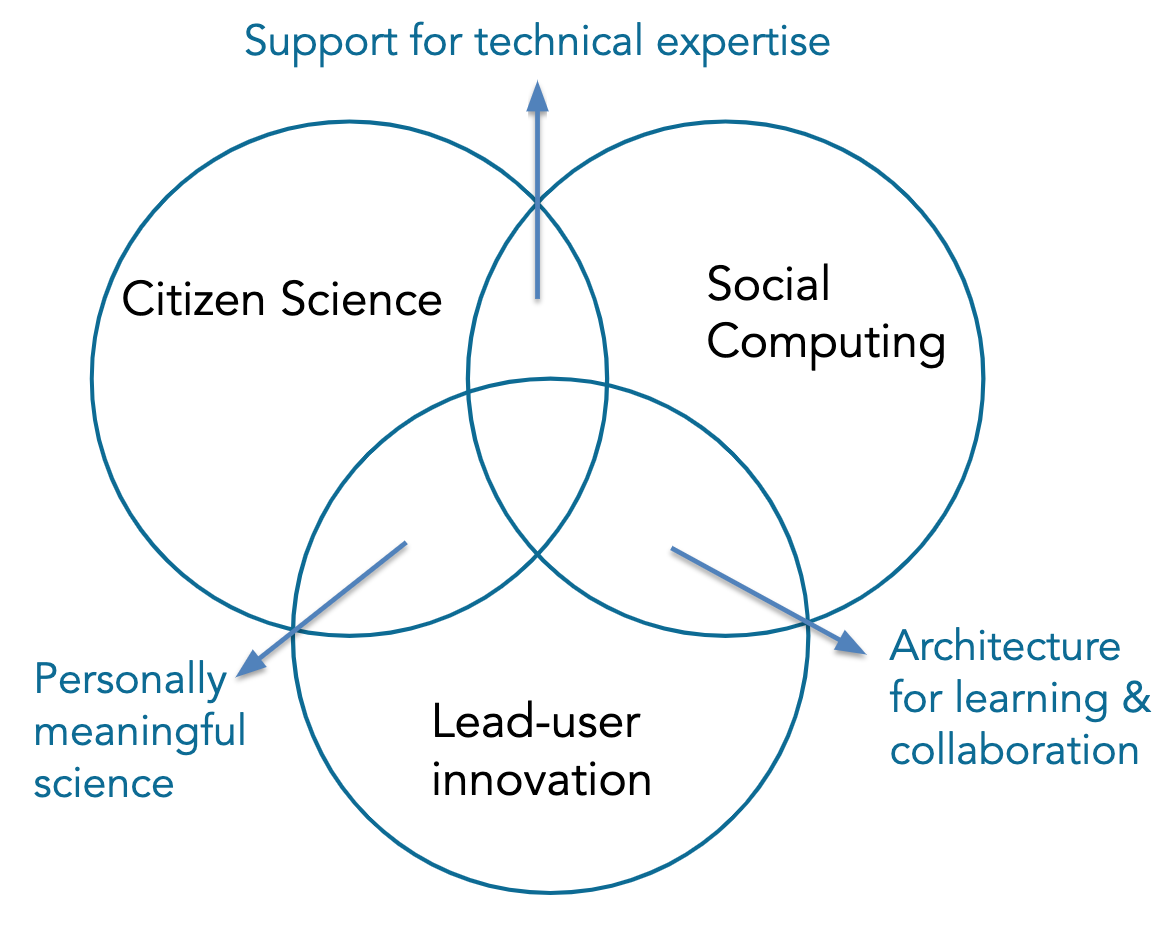
\includegraphics[width=0.6\textwidth]{figures/2-related/venn.png}
  \caption[]
{This dissertation draws from and contributes to citizen science, lead-user innovation, and social computing\index{related-1}}
  \label{fig:related-1}
\end{figure}

\vspace{0.25in}

%So, we find that there are three main challenges for citizen science: 1) make it personally meaningful, 2) deepen the contributions that citizens can make. 3. 1. Improve the quality of poor contributions — and improve the quality of max contributions     1. — hockey stick curve 
%%%%%%
\section{Science is increasingly networked but misses people’s lived experience }
Science is increasingly networked, multidisciplinary, and
open~\cite{Pandey2017}. For instance, \textit{LIGO}’s pathbreaking discovery of
gravitational waves brought together over 100 researchers
from over 100 institutions across 18 countries (ligo.org/about). 
Scientists increasingly share data and results faster (arxiv.org). 
Large scientific projects, like the \textit{Human Genome Project}, 
took to agile science by sharing methods, data, and insights to 
collaboratively speed discoveries. Scientists also form global 
collaborations to accelerate research in nascent scientific domains, 
like the Earth Microbiome project (earthmicrobiome.org).
At its best, institutional science has benefitted immensely
from large-scale global collaboration. Complementing this success,
many online projects enable people to help scientists~\cite{Nielsen2012}: annotating 
scientific papers~\cite{Good2013}; labeling galaxies~\cite{JordanRaddick2013}; and providing microbiome 
samples~\cite{McDonald2018}, CPU cycles (worldcommunitygrid.org), or personal data (openhumans.org). 
Efforts to further expand participation in scientific research are bearing fruit: \textit{Lab in the Wild} 
recruits anyone with an internet connection for behavioral studies~\cite{Reinecke2015}; and \textit{All of Us} aims 
to recruit one million Americans from all strata of society (allofus.nih.gov). Such collaborative efforts from experts 
and citizens suggest a new model for scientific work.

Often, when citizens participate in science, it is as \textit{embedded sensors} that 
are aggregated by experts. Public involvement in scientific endeavors continues
to be largely limited to performing tasks just beyond the reach of computers.
A classic example is \textit{Audubon}’s Christmas bird count, run since 1900
~\cite{Audubon2016}. Online examples include reporting flower blooms in
\textit{Project Budburst}~\cite{BoulderColorado2016}; recording wildlife activity~\cite{Faridani2009a};
identifying galaxies from satellite imagery in \textit{GalaxyZoo}~\cite{Zooniverse2007}; 
and biochemistry games: finding protein structures in \textit{Foldit}~\cite{Cooper2010}, 
synthesizing RNA molecules in \textit{EteRNA}~\cite{Lee2014}, and aligning 
nucleotide sequences in \textit{Phylo}~\cite{Kawrykow2012}. Distributed 
data contributions from people around the world—browsing online~\cite{Coviello2014}, using activity trackers, and joining scientific projects—have enabled valuable insights on topics including 
obesity~\cite{Althoff2017}, aesthetic preferences~\cite{Reinecke2014a}, sleep~\cite{F.lux2019}, and the human microbiome~\cite{McDonald2018a}. At their
best, these citizen science platforms yield novel insights.
For example, \textit{Foldit} players discovered protein structures
that helped scientists understand how the AIDS virus reproduces~\cite{Coren2011}. Why have such collaborative efforts succeeded?


%Different people provide different expertise that can vet claims and  fix mistakes~\cite{kane2009s}.
Collaboration benefits creativity when it brings different
 perspectives that build on each other; it impedes creativity (or worse, causes regression) 
when—through groupthink—it spreads biases rather than removing them~\cite{starbird2014rumors}. 
A humbling example of the power of fresh eyes: volunteer citizen scientists identified a new class of 
galaxies (\textit{green pea} galaxies) after researching green blots on \textit{Galaxy zoo} images; 
experts had dismissed these images as apparatus error~\cite{cardamone2009galaxy}.
This volunteer-led discovery demonstrates the need for fostering independent perspectives 
while simultaneously cultivating sufficient knowledge for meaningful domain contributions. 
Such collaboration requires strategic isolation: roviding just enough scaffolding to keep 
biases independent, while not stifling original ideas for bottom-up knowledge creation.

%This dissertation draws on the idea of people using  cognitive surplus to collaboratively answer scientific questions~\cite{Bonney2009}.


%%%% - where does this go
%Such bite-sized contributions is not without reason—a lot of
%scientific work requires deep conceptual knowledge and 
%training in scientific process to perform useful work. Most
%citizens lack the time, resources, and motivation to develop
%narrow, unique skillsets. Expanding the depth and breadth of work 
%performed by citizen science communities would be useful.

%\subsection{Citizen Scientists: From Collectors to Experimenters}
\subsection{Opportunity: Can people be scientists rather than just sensors?}
Citizens have successfully solved expert-defined problems as sensors or algorithms with a 
row-filling model of contribution.
In the quest to get people to track, measure, accumulate, or
sort both digital and analog data, citizen science has overlooked the massive 
opportunity of leveraging people’s unique advantages: our skills as reflective, 
creative thinkers who generate theories about the world, including ourselves.
People can offer more than just their data and perceptual
skills: they create theories, right or wrong, about a wide
range of topics including emotions~\cite{Johnson-Laird1992a}, motivation~\cite{Markus1991}, or
diet. These may be observational theories~\cite{Kempton1986}, folk theories
passed in a family/culture across generations~\cite{Gelman2011}, or ideas
brainstormed in online communities~\cite{23andme2016}. Perhaps, these intuitions 
can provide a starting point for independent, participatory experience that also assists the scientific community.

When are such personal experiences worth paying attention
to? For every intuition proven right, many more may be
closer to snake oil — e.g., the widespread belief in the utility
of probiotics despite limited evidence~\cite{Bonifait2009}. The global internet
increases the proliferation of both powerful and questionable
ideas: sharing speculation is fast while evaluation remains
slow. Moreover, people develop intuitions of cause and effect
that may or may not be correct. Current online forum
designs prioritize discussion — sharing personal details in
long, free-flowing text — over structure, succinctness, learning,
and potential scientific utility~\cite{Thomas2002}.

Advances in precision medicine have demonstrated the need
to engage people in uncovering and sharing insights~\cite{Aronson2015}. People
are highly motivated to improve their health outcomes,
more so if they suffer from a condition that severely affects
their quality of life, naturally forming communities. For example,
patients from the Amyotrophic Lateral Sclerosis
(ALS) community on \textit{Patients Like Me} (patientslikeme.com)
organized a study to track effects of Lithium on their symptoms
~\cite{Wicks2011}. This is not surprising; lead users excel at tackling
\textit{need-intensive} problems where they can use their lived
experiences to identify problems, try solutions, and readily
observe the effects~\cite{VonHippel2005}. Other organized communities like
\textit{Quantified Self} hope to uncover lifestyle patterns that may
improve their productivity and health outcomes. The word
‘self’ belies the fact that such movements are highly collaborative:
amateurs frequently share experiences and invite
feedback on online fora (patientslikeme.com) and blogs
(ibsgroup.org). Millions follow these ideas and some incorporate
these intuitions in their lives. What kinds of scaffolds
and structure may help people generate better ideas and implement them as actionable plans that
enable researchers to identify promising insights?

%How can people expand their insights into scientific work?

Most scientists develop their skills through an apprenticeship-
based graduate school experience. Apprenticeships emphasize
hands-on experience with individualized, taskspecific
feedback~\cite{schon1984reflective}. Scientists possess a wealth of declarative
knowledge about their domains (e.g., how to set up a
randomized controlled trial), and also procedural knowledge
—some narrow, some broad —towards getting things done
(e.g., improving fMRI signal intensity by having participants
consume cocoa beforehand~\cite{Francis2006}). This dissertation explores how
online learning and process training systems, combined with
peer collaboration, can help people learn similar skills that
can be useful in scientific domains.
%So, we find that there are three main challenges for citizen science: 1) make it personally meaningful, 2) deepen the contributions that citizens can make. 3. 1. Improve the quality of poor contributions — and improve the quality of max contributions     1. — hockey stick curve 
%WOULDN'T IT BE GREAT TO HAVE PEOPLE DESIGN AND RUN EXPERIMENTS AS AN INSTANCE OF COMPLEX SCIENTIFIC WORK
%Link to lead users -- people already doing personally meaningful work.. 

%%%%%%%%%%%%%%%%%%
\section{Lead users Succeed When They Know What to Do and How to Do It}
%“Lead users are rarely experts by themselves. They are novices who find themselves at the right place, with the right tools (that they might have created themselves), and who have the courage to follow through.” Lead users have created different—and in some cases better designs— than experts. 

%examples: UN example (see eric vh)

Lead-user innovation is both an inspiration and an application area for this dissertation. Lead users are
users of a product (or service) who experience advanced needs unmet by existing products~\cite{VonHippel2005}. The
power of lead-user innovation is that lived experience, a tight feedback loop, and strong personal
motivation can yield different and sometimes better products than experts [32]. For example, diabetes
patients have improved insulin delivery [47] and snowboarders have improved their binding
ergonomics. Lead users also collaborate online to build software
(github.com), create novel hardware \& reference designs
(openaps.org), and share personal data (quantifiedself.com,
openhumans.org). Some go further still, e.g., the transcranial
direct-current stimulation community draws ideas from scientific
papers to attempt self-experiments (reddit.com/r/tDCS). In a few exceptional cases, lead users have authored
scientific papers, e.g., Open Artificial Pancreas creator
Dana Lewis discussed the benefits and challenges of first-generation
automated insulin delivery at the 2016 American
Diabetes Conference~\cite{DanaLewis}.

Why do people do this? Curiosity, personal learning, and social
comparison are three reasons~\cite{Reinecke2015}. A massive interest in
personal genomics (over 1 million 23andme participants)
and the human microbiome (13,000 \textit{American
Gut} participants) demonstrates people’s yearning for self-understanding.
Users of these platforms send data, answer survey questions,
and discuss on fora. Some even use online lectures to understand
concepts of genes, phenotypes, and microbiota~\cite{23andMe2017, Knight2016}. 

\subsection{Opportunity: Providing lead users the expertise to tackle complex knowledge work}
Sometimes, having a different background
 than experts can be beneficial. Shared knowledge is great when it’s right, but blocks progress
 when wrong. When false assumptions limit experts, at least some novices are likely to be 
\textit{uninfected}. The converse also holds, and much more often: novices are also uninfected
by all the knowledge that enables experts to innovate. Lead users have an advantage when the key ingredient is experience intensive; experts retain the
advantage for \textit{solution-intensive} innovations [32]. In a large distributed community, 
there’s often someone who happens to have important relevant knowledge, usually 
drawing on a relevant but distant domain. Having many people work on the same problem 
increases the odds that one will break through. Drawing on secondary expertise as 
inspiration can be an important agent of creativity because almost by definition, the
 combination is rare~\cite{Boden2004}. 
%For example, GalaxyZoo volunteers discovered ‘green pea’ galaxies overlooked by scientists who mistakenly assumed the green hue was merely an imaging artifact~\cite{Tinati2015}. 

Community-driven approaches to understand personal
health and well-being largely reside outside the realm
of institutional science and medicine. While some fads and beliefs are 
questionable at best, on occasion communities
break new ground that may provide widespread value,
such as fecal transplants to alleviate \textit{Clostridium difficile} infection
symptoms~\cite{Brandt2012}. Some doctors recommend that patients
track their symptoms and reflect upon them to find
insights. Putting people in charge can help them find significant
relief for ailments like chronic migraine~\cite{Gawande2017} and provide
researchers and clinicians with useful patient data
(smartpatients.com). Insights from N\Hair=\Hair1 studies have helped
crack scientific puzzles about the working of the mind~\cite{V.S.Ramachandran1998},
heart, and microbes~\cite{Weisse2012}. 

Personal needs and challenges can be highly motivating but performing complex work still requires multiple rounds of trial and error. 
People need to know the genre of work and implement it correctly.  Professionals have the advantages of training, conceptual knowledge, 
pre-existing organizational structure for 
collaboration and support, and direct access to resources. Lead users either seek these resources from others or need to create them. 
Providing a correct and complete model for complex, structured activities might reduce efforts and improve the quality of results.
This dissertation reduces the gap between lead users' ideas and implementation by providing templates for 
genre work using just-in-time training and a collaboration platform to find others. This dissertation focuses on enabling people transform their idea to a controlled experiment as opposed to 
self-tracking or informal iteration which is the focus of most current citizen-led work in health.

\subsection {Case: Scientific experimentation is difficult}
While public contributions have supported institutional science; it’s rare for citizens to design
their own experiments. A number of health and behavioral research projects enlist citizens as helpers (e.g., \textit{HabitLab} [43]). 
\textit{CivilServant} enables online communities’ 
moderators to test policy ideas; moderators share these ideas with researchers who transform 
them to study designs [51]. Through the \textit{PatientsLikeMe} website (patientslikeme.com), citizens 
and scientists created a study investigating whether consuming lithium alleviated ALS symptoms [64]. 
While an initial scientific study had provided positive benefits, both this citizen science study and 
a subsequent university study did not find benefits. \textit{Tummy Trials} asked 
participants to generate health questions, introducing a protocol for self-experimentation 
combining ideation and self-tracking [36]. In all these cases, citizens rely on experts to provide sound experimental design.

Why is experimentation hard?  Despite a predetermined goal and a formalized process, experimentation
requires making situationally-appropriate decisions. A dependent variable may produce crisp
numbers but feedback on the experiment design itself is more multifarious. Good experiment
design is inherently user centered: how will participants interpret the instructions? Experiment
designers need awareness of others’ interpretation of their ideas and asks. Feedback and iteration
might be key to creative success, especially for novices. Providing feedback on experiment
designs requires knowing the success criteria and how to
help improve.  Feedback can be provided by experts~\cite{dow2012shepherding, schon1984reflective}, peers~\cite{Boud1995, Kulkarni2015b}, software~\cite{Dantoni2015, Head2017}, or even oneself~\cite{Boud1995,schon1984reflective}. While feedback from novices can
potentially improve both structure and content, it can also emphasize superficial issues over the
underlying structure~\cite{chi1981expertise}. Finally, successfully running an experiment
requires managing multiple processes such as random
assignment, anonymizing participant details, and sending
instructions and reminders for data collection.

%%%%%%%%%%%%%%%%%%%%%%%%%%%%%%%%%%%%%%%%%%%%%%%%%%%%%%%%%%%%%%%%%%%%
%But to understand that let's look at social computing ideas...

\section{Social Computing and Crowdsourcing Architectures for Complex Work}
Canonical crowdsourcing breaks larger tasks into microtasks; algorithms specify the division,
dependency, and agglomeration activities while workers perform small tasks supported by task-specific
guidelines~\cite{kittur2012future}. Leveraging existing expertise is one approach for complex knowledge work. One strategy
directly employs experts’ just-in-time feedback to improve crowd work~\cite{dow2012shepherding}. Workflows manage
experts for open-ended work like developing interactive prototypes~\cite{Retelny2014}. 
\textit{Flash Organizations} uses automated hiring, a hierarchy with a central leader, and optional 
team leaders for collaborative projects like product design~\cite{Valentine2017}.
Another strategy creates roles that enable more experienced crowd members to orchestrate
the work. \textit{Ensemble} supports leaders in guiding and constraining crowd 
contributions~\cite{Kim2014e}. Role-based approaches confer three benefits: 1) clean 
delineation of responsibilities improves chances of task completion, 2) clustering similar tasks 
reduces overhead and increases consistency; 3) people can decide their contribution levels. 
However, experts are expensive, in short supply, and sometimes prone to groupthink. 

Carefully-constructed interfaces can aid novices with task-specific expertise to solve problems 
that only experts previously could. \textit{Foldit} introduced 3D game for specifying low-energy protein 
structures via direct manipulation~\cite{Cooper2010}. Making a challenge visually salient is an 
effective way to on-board novices. For tasks that don’t have as a crisp visual analogue as protein
folding, people need better conceptual support. Prior work has explored collaborative hypothesis generation and testing on pre-existing data sets
~\cite{luther2009pathfinder,willett2011commentspace}. This dissertation offers a 
complementary contribution: enabling citizens to generate data on topics of personal interest.

One way to make complex tasks manageable is to divide them into distinct phases. 
Touchstone demonstrates the power of a semi-automated workflow integrating experiment 
design, testing, and analysis~\cite{Mackay2007}. Crowdsourcing has similarly innovated by 
creating distinct phases: break larger tasks into microtasks; algorithms specify the division, 
dependency, and agglomeration activities while workers perform small tasks supported by 
task-specific guidelines~\cite{lasecki2012real}. From these systems, our work draws the 
idea of dividing experimentation into multiple tasks—some self-sourced, others 
crowd-sourced; and introduce just-in-time domain expertise to perform these tasks. 

 
%How might groups of novices perform complex work like experimentation?
%Systems like Foldit and EteRNA powerfully show  how carefully-constructed interfaces provide
%novices with the task-specific expertise to solve problems that only experts previously 
%could~\cite{Cooper2010, Lasecki2012, Lee2014, Zooniverse2007}.

%%%%%%%
%%building up solution space - more work
\subsection{Learning resources at the right time}
Providing just-in-time supports, step-by-step instruction, and showing helpful supportive
 information are core ideas in instructional design~\cite{Kirschner2008}. Crowdsourcing 
systems leverage interactive guidance for specific tasks. For example, \textit{CrowdLayout} and 
\textit{Cicero} provide guidelines and static rules that workers use these to reason about their choices
 and improve network layouts~\cite{chen2019cicero, Singh:2018:CCD:3173574.3173806}. 
Others like \textit{CrowdSCIM} and \textit{Crowdclass} scaffold pre-task interventions~\cite{Lee2016,wang2018exploring}. 
While learning resources are distributed across the internet, they are rarely integrated with the task. 

Creative, open-ended work has rich pedagogical value. Online work, like 
online learning, requires appropriate scaffoldings, such as rubrics
~\cite{Boud1995, Kulkarni2013peer}, decision trees~\cite{Lee2016,Yu2006}, 
tutorials~\cite{Andersen2012}, and quick expert guidance~\cite{dow2012shepherding}. 
Similar to general critique of pure discovery learning~\cite{Mayer2004}, simply 
asking participants to \textit{figure it out} would be poor pedagogy. Hence, this dissertation
introduces a guided discovery learning approach as Mayer advocates: expert-curated 
learning materials help participants start, with discovery following. Such integration 
offers a problem-based learning experience with context and 
motivation for the material students learn~\cite{Savery1995}. In principle, these 
real-world problems also provide a yardstick for measuring learning. 

This dissertation introduces support during the task itself for those with little-to-no mental model of the knowledge domain. 
Like the \textit{Shepherd} review-writing system~\cite{dow2012shepherding}, this dissertation provides just-in-time support. 
There are two key differences: 1) this work scaffolds the entire creation process, not just the post-draft feedback
 stage, and 2) it does not draw on expert time – the knowledge is implemented in the software itself. 
%todo-repeated too many times


%%%%%%%%%%%
\section{Microbiome research: a petri dish for personally meaningful scientific work}
The human microbiome is the collection of all microbes and
their genetic components in and on our bodies. It is highly
personal: each of us hosts a different collection of microbes,
and this collection is influenced by our environment, diet,
health, lifestyle, and genetics. A major scientific effort is to
better characterize and understand this diversity and the
causal factors for it (hmpdacc.org). Understanding the human microbiome requires insights
into people’s lifestyles. Microbiome science is nascent, highly contextual, and personally motivating.
However, research has only scratched the surface of understanding the microbiome and using it 
to improve our wellbeing. Engaging diverse participants at scale can potentially yield exciting new results.


The \textit{American Gut Project} (americangut.org) offers a
crowdsourced opportunity for people to get a microbiome
sampling kit~\cite{KnightLab2016a}. AGP
participants contribute their samples for bacterial marker
gene sequencing and analysis~\cite{Debelius2016}. Participants then receive
a summary of their results with all their raw data. Anonymized data is publically available.

To date, more than 13,000 people have participated.
Participants submit both a physical sample and fill out
a survey. AGP seeks to build a comprehensive map of the human microbiome, and identify
its healthy and unhealthy components. Analysis has revealed lifestyle-microbiome correlations
of dog ownership and beer or vegetable consumption,
among others.

\subsubsection{People hold the key to understanding the gut microbiome}
The structure of the human microbiome is influenced by many factors, including age, genetics, diet, and xenobiotic and antibiotic use~\cite{Gill2006}. The gut microbiome in particular plays an important role in metabolism and immune system development, and some microbiome dysbioses have been associated with diseases such as obesity, inflammatory bowel disease, type I and type II diabetes, autism, multiple sclerosis, and malnutrition~\cite{Cho2012}. The human microbiome is impossible to understand without information about its host~\cite{Debelius2016} and many influence factors remain unknown. Teaching people about the gut microbiome and having them guess associations between the microbiome and health and disease states can potentially accelerate the process of discovering links between diet, disease, and lifestyle factors and the gut microbiome.

Currently, the topics for scientific investigation are handpicked
by a small group of scientists. Can opening up the
scientific process to the world yield additional insights?
How can people’s situated knowledge supplement institutional
science? This dissertation provides systems and techniques for novices to complement experts in creating new knowledge about the microbiome. \\

%Crowd workers perform better when they understand their efforts’ importance. For example, Mechanical Turk workers analyzing radiology images performed better when told of the medical purpose: finding cancerous tumors~\cite{Chandler2013}. Motivation can also be personal. For example, 23andMe is a genetic testing site and online service that includes a discussion board. On this forum, a user reported disliking the sounds of others eating. She’s not alone; a 23andMe survey found 16,000 users with the same condition and a predictive genetic similarity among them~\cite{23andMe2016}.

This chapter provided an overview of related research; chapters dedicated to specific systems discuss additional research that informs that design of those systems. This dissertation explores integrating learning in social computing for complex, creative work with two goals in mind: efficacy of the resulting systems (i.e. usability, correctness, and existential evidence) and generality of the underlying techniques upon which the tools are built.
\chapter{Collaboratively Generating Ideas}

\begin{quote}
\emph{Learners worldwide collectively spend millions of hours per week testing their skills on assignments with known answers. Might some of this time fruitfully be spent posing and exploring novel questions? This chapter investigates an approach for learners to contribute scientific ideas}. The Gut Instinct system embodies this approach, hosting online learning materials and invites learners to collaboratively brainstorm potential influences on people’s microbiome. A between-subjects experiment compared the performance of participants who engaged in just learning, just contributing, or a combination. Participants in the learning condition scored highest on a summative test. Participants in both the contribution and combined conditions generated novel, useful questions; there was not a significant difference between the two. Though participants in the combined condition both learned and contributed, this setting did not exhibit an additive benefit, such as better learning in the combined condition. 
%These results highlight the promise and difficulty of double-bottom-line learning experiences.
\end{quote}

\begin{figure}[h]
  \centering
  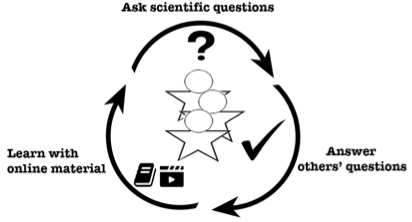
\includegraphics[width=0.6\textwidth]{figures/gutinstinct/gi-1.png}
  \caption[A dual objective: integrating citizen science and online learning]
{A dual objective: integrating citizen science and online learning\index{gi-1}}
  \label{fig:gi-1}
\end{figure}

\vspace{0.25in}


%%%%%%%%%%%%%%%%%%%%%%%%%%%%%%%%%%%%%
\section{The Promise of Citizen Science with Learners}

%\begin{wrapfigure}{r}{0.5\textwidth}
%  \centering
%  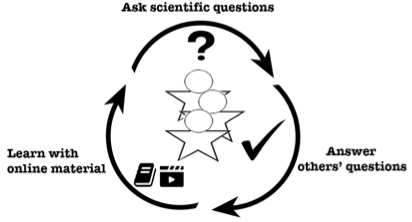
\includegraphics[width=0.5\textwidth]{figures/gutinstinct/gi-1.png}
%  \caption[A dual objective: integrating citizen science and online learning]
%{A dual objective: integrating citizen science and online learning\index{gi-1}}
%  \label{fig:gi-1}
%\end{wrapfigure}
People worldwide have theories about their health, environment, interpersonal interactions, and myriad other topics~\cite{Gelman2011}. Some of these folk theories encapsulate generalizable insights and wisdom; many others are completely false; and some are in between~\cite{Kempton1986}. How might we harvest and assess such intuitive theories to extend human knowledge, especially in domains where science is limited?  Worldwide, students collectively spend millions of hours a week testing their skills on assignments with known answers~\cite{Shah2015}. This community could be a potentially powerful resource. Repurposing even a small fraction of this effort towards scientific inquiry could pay significant dividends. 

Our intuition is that scientific crowdsourcing will most usefully contribute to domains where science is nascent and/or highly contextual. Knowledge of the human microbiome is both. While everyone has a gut full of microbes, its causal influences remain largely unknown. The Human Microbiome Project and other studies have begun revealing its diversity and impacts~\cite{Consortium2012, Consortium2013}. The world could benefit greatly from a more comprehensive understanding of the microbiome, what influences its composition, and the impact our gut has on our health. Understanding how people live may help build causal models. For example, rheumatoid arthritis patients have altered gut and oral bacteria~\cite{Zhang2015}. Might changing their gut reduce their symptoms? As in many scientific domains, people’s initial intuitions about what affects their gut are often poor. Does this improve with education? Could learners collectively advance human understanding in this domain? This chapter explores the potential of coupling online citizen science with learning materials to create scientific questions (Figure~\ref{fig:gi-1}). 

The main contribution of this chapter is \textit {demonstrating that a crowd of online non-expert learners can collaboratively perform useful scientific work}. To investigate its efficacy in practice, we have built a web system, Gut Instinct, which brings together learners to perform useful collaborative brainstorming on a citizen science project while developing expertise. A between-subjects experiment compared three variations of Gut Instinct: a contribution focus, a learning focus, and a combined condition. Participants did indeed perform useful creative work. For example, they generated 10 distinct questions that mirror recent scientific discoveries~\cite{KnightLab2016}. However, the combined condition did not show additive benefits. 

%\begin{wrapfigure}{r}{0.5\textwidth}
%  \centering
%  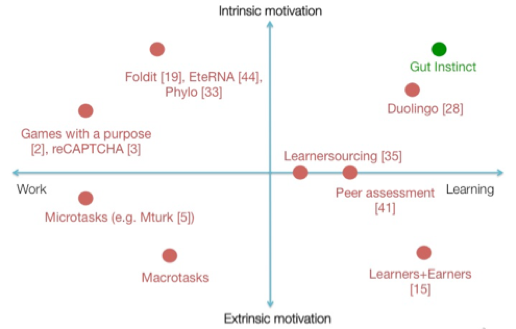
\includegraphics[width=0.5\textwidth]{figures/gutinstinct/gi-2.png}
%  \caption[Crowd systems/techniques place different emphasis on
%work and learning]
%{Crowd systems/techniques place different emphasis on
%work and learning. Some, like Mechanical Turk~\cite{Amazon2016}, emphasize
%work over learning. Crowd approaches also vary in their motivation.
%Games like Foldit~\cite{Cooper2010} leverage participants’ motivation
%to perform altruistic work while having fun. Gut Instinct helps
%participants learn about the gut microbiome while contributing
%towards the altruistic purpose of helping researchers better
%understand it.\index{gi-2}    \textbf{Refs for the fig: ~\cite{Chen2016b}}}
%  \label{fig:gi-2}
%\end{wrapfigure}


\subsection{Leveraging Crowdsourcing successes}
Collectively aggregating many people’s responses can produce faster, better, and more reliable results---at much larger scale---than lone individuals can, at least when errors and biases are independent events~\cite{Surowiecki2005}. Canonical crowdsourcing tasks have clear right or wrong answers – like whether two images represent the same product, whether an image region contains a feature, or what street number is written on a sign.

Distributing labor redundantly across multiple workers also guards against individual shortcomings~\cite{Snow2008}. For example, workers using the Soylent crowd-powered document editor found a typo late in a paper that eluded all eight authors and six reviewers~\cite{Bernstein2010a}. Why? In later pages, fatigue can reduce attention to detail. Because individual crowd workers saw only a small piece of the document, their collective attention to detail remained constant throughout. This illustrates how a collection of novices offers complementary contributions to experts, often in small but nonetheless useful ways. 

%Sometimes, having a different background than experts can be beneficial. Shared knowledge is great when it’s right, but blocks progress when wrong. When false assumptions limit experts, at least some novices are likely to be “uninfected”. For example, GalaxyZoo volunteers discovered ‘green pea’ galaxies overlooked by scientists who mistakenly assumed the green hue was merely an imaging artifact~\cite{Tinati2015}. The converse also holds, and much more often: novices are also “uninfected” by all the knowledge that enables experts to innovate. In a large distributed community, there’s often someone who happens to have important relevant knowledge, usually drawing on a relevant but distant domain. Such distributed efforts are a type of lead-user innovation~\cite{VonHippel2005a}. Having many people work on the same problem increases the odds that one will break through. Drawing on secondary expertise as inspiration can be an important agent of creativity because almost by definition, the combination is rare~\cite{Boden2004}. Open \& crowd innovation builds up on contributions by diverse online participants, and a ‘bubbling up’ process for strong ideas~\cite{Yu2012}. Our novel contribution is an explicit integration of learning.

%Crowd workers perform better when they understand their efforts’ importance. For example, Mechanical Turk workers analyzing radiology images performed better when told of the medical purpose: finding cancerous tumors~\cite{Chandler2013}. Motivation can also be personal. For example, 23andMe is a genetic testing site and online service that includes a discussion board. On this forum, a user reported disliking the sounds of others eating. She’s not alone; a 23andMe survey found 16,000 users with the same condition and a predictive genetic similarity among them~\cite{23andMe2016}.

%Creative, open-ended work has rich pedagogical value. Online work, like online learning, requires appropriate scaffoldings, such as rubrics~\cite{Boud1995, Kulkarni2013peer}, decision trees~\cite{Lee2016,Yu2006}, tutorials~\cite{Andersen2012}, and quick expert guidance~\cite{dow2012shepherding}. Similar to general critique of pure discovery learning~\cite{Mayer2004}, simply asking participants to “figure it out” would be poor pedagogy. Hence, Gut Instinct introduces a guided discovery learning approach as Mayer advocates: expert-curated learning materials help participants start, with discovery following. Recruiting learners as citizen scientists offers a Problem-based learning experience with context and motivation for the material students learn~\cite{Savery1995}. In principle, these real-world problems also provide a yardstick for measuring learning. 

\begin{figure}[h]
  \centering
  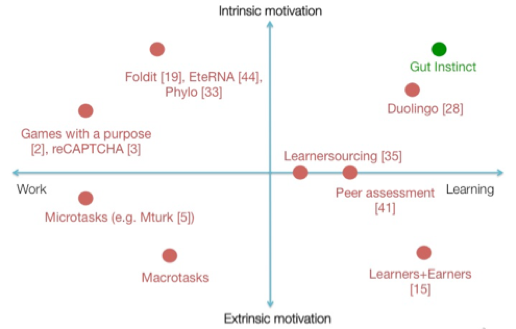
\includegraphics[width=0.7\textwidth]{figures/gutinstinct/gi-2.png}
  \caption[Crowd systems/techniques place different emphasis on
work and learning]
{Crowd systems/techniques place different emphasis on
work and learning. Some, like Mechanical Turk~\cite{Amazon2016}, emphasize
work over learning. Crowd approaches also vary in their motivation.
Games like Foldit~\cite{Cooper2010} leverage participants’ motivation
to perform altruistic work while having fun. Gut Instinct helps
participants learn about the gut microbiome while contributing
towards the altruistic purpose of helping researchers better
understand it.\index{gi-2}    }
  \label{fig:gi-2}
\end{figure}

%%%%%%%%%%%%%%%%%%%%%%%%%%%%
\subsection{Dual objective functions in learning and crowdsourcing}
Combining university classes in psychology with editing
Wikipedia articles led to improvement in the scientific
content of over 800 Wikipedia articles while students
learned about the topic they edited~\cite{Farzan2013}. Similarly, Kim et
al. asked learners to create how-to video segments as part
of an online curriculum~\cite{Kim2015f}; the student-created videos
then became a learning resource for the next cohort. 

Some crowdsourcing offers a dual objective: user-facing
goals include fun (e.g., Peekaboom~\cite{VonAhn2006}), authentication
(reCAPTCHA~\cite{Ahn2008}), and learning (Duolingo~\cite{Hacker2014}). Under the
hood, these tasks simultaneously label images, transcribe
text, and translate phrases. Such crowd work can also bootstrap machine learning~\cite{Bernstein2012c}. This paper is distinct from prior
work (Figure~\ref{fig:gi-2}) in leveraging people’s individual lived
experience, knowledge, context, and folk theories, rather
than treating people as interchangeable respondents.

%%%%%%%%%%%%%%%%%%%%%%%%%%%%%%%%
\section{Hypotheses}
This chapter investigates an approach for a community of learners to collaboratively create scientific theories. Learning is any endeavor that seeks to increase a participant’s knowledge. In this submission---like many MOOCs---watching videos is the main form of learning, \& quizzes are the main assessment. Work is any endeavour where the outcome has value. In this submission, authoring \& answering questions are the main work forms. This study operationalized engagement as time spent. We hypothesized that doing useful work on real-world problems helps learning, and vice versa. Specifically:

\textbf{H1. Learning improves quality of work on relevant problems.}
Learning, by definition, improves performance on similar tasks. Strangely, transfer to novel tasks (like creating new \& different questions) is famously uneven~\cite{Boden2004}---and sometimes detrimental. H1 tests whether learning would improve work (e.g., novel question creation) because it marries lived knowledge (about diet, health, etc.) with a conceptual framework about the gut’s role.

\textbf{H2. Working on relevant real-world problems improves learning.}
H2 tests whether working improves learning because it increases motivation \& provides an immediately relevant \textit{host context} for new knowledge.
 
\textbf{H3. Working while learning improves learners’ engagement with the learning material.} 
For similar reasons, we hypothesized that working alongside learning would increase engagement because the two endeavors both \textit{get the wheels turning} in hopefully complementary ways.

We test these hypotheses in the context of brainstorming potential causal relationships in the human gut microbiome. 

%%%%%%%%%%%%%%%%%%%%%%%%%%%%%%%%%%%%
\section{The Gut Instinct System}
Gut Instinct is a collaborative system with a dual objective: help people learn about the gut microbiome, and catalyze the creation of a list of factors that may be associated with gut microbiome differences (Figure~\ref{fig:gi-3}). People anonymously post questions about lifestyle and health for peers to answer. Learners both ask \& answer questions, there are
no distinct workers. These questions and discussions provide researchers cues to build associations between lifestyle and the microbiome.
Gut Instinct is a web application built with Meteor (http://www.meteor.com). The front-end uses Angular (http://www.angularjs.org) and is stylized with Materialize (http://www.materialize.css).

\begin{figure}[h] 
  \centering
  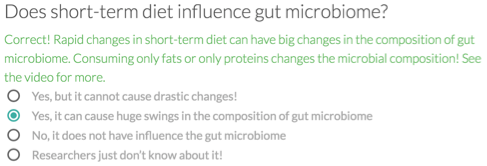
\includegraphics[width=1.0\textwidth]{figures/gutinstinct/gi-3.png}
  \caption[Gut Instinct is a web system to learn about the gut microbiome and create causal theories about gut microbiome]
{ Gut Instinct is a web system to learn about the gut microbiome and create causal theories about gut microbiome (a) A discussion board where learners add their questions and discuss them with other learners (b) "Add question" box for people to add their own questions, (c) A tutorial video showing how gut microbiome varies across countries with different food habits~\cite{Yatsunenko2012}\index{gi-3}}
  \label{fig:gi-3}
\end{figure}

\subsection{Curating content based on topics}
Gut Instinct provides expert-approved learning material including online lectures, science articles and research papers. Participants add articles they feel are useful, which can be fact-checked by experts. The gut microbiome is an active area of research with new results being generated rapidly. A popular MOOC provides an introduction to science the gut microbiome including its relation to some lifestyle choices~\cite{Knight2016}. Popular online articles about the microbiome are split between providing correct, useful information and clickbait articles without scientific validity.

%\begin{wrapfigure}{R} {0.5\textwidth}
%  \centering
%  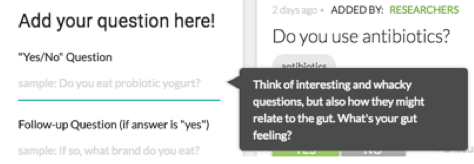
\includegraphics[width=0.5\textwidth]{figures/gutinstinct/gi-4.png}
%  \caption[A question on Topics page for diet to test understanding of the learning material]
%{A question on Topics page for diet to test understanding of the learning material \index{gi-4}}
%  \label{fig:gi-4}
%\end{wrapfigure}

Gut Instinct organizes the learning material based on topics such as diet or antibiotics. A topic-based classification of learning material provides two advantages: (a) People can deeply focus on the topics that interest them, and (b) Topics related to specific lifestyle aspects can trigger specific questions. The topics pages include videos and articles about diet, antibiotics, probiotics, physiology, and genetics based on vetted content from online sources. Quick multiple-choice questions with detailed feedback at every topic page help people test their understanding (Figure~\ref{fig:gi-4}). Overall, these elements of the interface form the learning part of the system.

\begin{figure}[h]
  \centering
  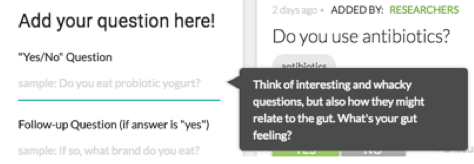
\includegraphics[width=0.7\textwidth]{figures/gutinstinct/gi-4.png}
  \caption[A question on topics page for diet]
{A question on topics page for diet to test understanding of the learning material \index{gi-4}}
  \label{fig:gi-4}
\end{figure} 

\subsection{GutBoard: Discussing and answering questions}
The GutBoard provides a discussion board with user-generated questions tagged by topics (Figure~\ref{fig:gi-3}a). People can browse questions, answer them, or participate in discussions. GutBoard presents unanswered questions first. The most popular questions (in terms of discussion comments) bubble to the top of the board.
 
\subsection{Adding questions}
Gut Instinct provides different tutorials, articles, and expert examples to help users contribute. Gut Instinct requires that questions have a two-part structure: a yes/no question followed by an open-ended elaboration. For example, the yes/no question “Do you take any meal replacements such as protein powders?” might be followed by “Do you take them on a daily basis?” This structure addresses two problems we witnessed with pilot users: (a) Some questions were actually multiple different questions, confusing readers (b) Readers had to read every question in full to understand what was being asked, even if the topic was not relevant to them. With this structure, every question has a single focused topic. Participants can also start a discussion about the question and provide relevant tags. “Add Question” box in Figure~\ref{fig:gi-3}b shows the interface.

\subsubsection{Nudges to think creatively and to stay on task}
\begin{figure}[h]
  \centering
  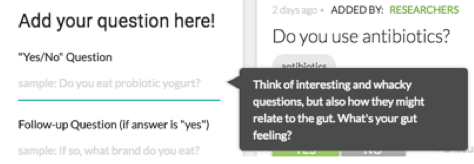
\includegraphics[width=0.5\textwidth]{figures/gutinstinct/gi-5.png}
  \caption[An example of a nudge used in Gut Instinct]
{An example of a nudge used in Gut Instinct to remind people of their role as a citizen scientist in raising interesting questions about the gut microbiome \index{gi-5}}
  \label{fig:gi-5}
\end{figure} 
Gut Instinct employs several best practices for increasing high-quality contributions~\cite{Jennett2014, Resnick2011}. It provides cues to teach participants to generate good questions. All parts of the Add Question box contained sample questions to help participants frame their questions that could be useful to them and to gut microbiome researchers (Figure~\ref{fig:gi-5}). To reduce user confusion, GutBoard was seeded with expert questions that set norms for the nature of questions. To provide a clear call to action, GutBoard was the default landing page and the only place to add or view questions. Every page had a tour that users could invoke anytime to learn its interface.

%todo-uncomment -- don't know what's wrong
%\begin{wrapfigure}{b} {0.5\textwidth}
%  \centering
%  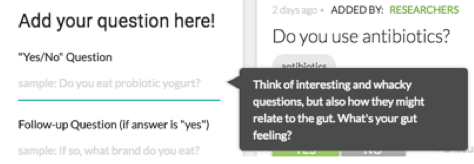
\includegraphics[width=0.5\textwidth]{figures/gutinstinct/gi-5.png}
%  \caption[An example of a nudge used in Gut Instinct]
%{An example of a nudge used in Gut Instinct to remind people of their role as a citizen scientist in raising interesting questions about the gut microbiome \index{gi-5}}
%  \label{fig:gi-5}
%\end{wrapfigure} 

%%%%%%%%%%%%%%%%%%%%%%%%%%%%%%%%%%%%%%%%
\section{Experiment: Work, Learning, \& Combined}

\begin{figure}[h]
  \centering
  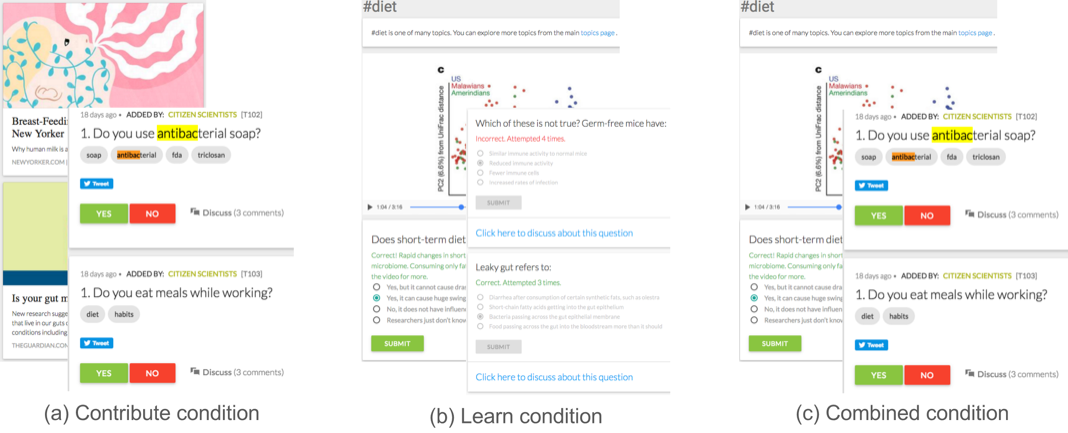
\includegraphics[width=1.0\textwidth]{figures/gutinstinct/gi-6.png}
  \caption[Three conditions for experiment]
{Three conditions for experiment. (a) Contribute condition where participants read some general articles about microbiome and added questions and answered others’ questions (b) Learn condition where participants saw curated topic videos (e.g. about diet) and answered practice problems from a Coursera class~\cite{Knight2016} (c) Combined condition where participants saw curated topic video, and added questions and answered others’ questions \index{gi-6}}
  \label{fig:gi-6}
\end{figure}

A between-subjects experiment compared the work and learning performance of participants across three different conditions: \textit{Contribute}, \textit{Learn} and \textit{Combined} (Figure~\ref{fig:gi-6}). In the Learn condition, participants were provided learning material and some practice problems, both curated from the Coursera microbiome class~\cite{Knight2016}). In the Contribute condition, they had access to brief pop-science articles to know basic details about the gut microbiome, and GutBoard for creating questions. In the Combined condition, subjects had access to both learning material from Coursera and the GutBoard. The GutBoard content was common to both conditions that used it (Contribute and Combined).

\subsection*{Method}
Participants were randomly assigned to one of the three conditions. Each comprised an individual lab session followed by web study, during which participants were asked to use the tool for 3 days. During this period, participants asked and answered each others’ questions in the tool.

\textit{Lab}: A researcher introduced the condition-appropriate Gut Instinct site. Participants were told there was no lower or upper limit on how much time to spend using the system. Each session comprised the following steps: (1) accessing the consent form, (2) seeing GutBoard/problems, (3) accessing topic videos/articles, and (4) participating in a short interview. The interview asked participants about their knowledge of the gut microbiome before using the system, and their experience using the system. The interview was tailored to the participant’s behavior: for example, if a participant did not click on Google Scholar references inside Gut Instinct but opened up a browser for web search, the interviewer would ask why.
 
\textit{Web usage}: Once all participants had completed the lab portion, the web application was opened to all participants for collaborative usage for three days. Gut Instinct sent email notifications about activity on the site, along with feedback on some questions raised on GutBoard such as providing links to research studies about effects of eating blueberries on the gut microbiome. 

After web usage, two independent raters (experts in human microbiome) rated the questions on novelty \& usefulness using the following workflow: (1) calibrate: rate 3 questions independently and discuss; (2) rate: independently rate all participant generated questions; (3) combine: discuss ratings where different \& develop a common score. The discussion in step 3 was valuable for adding to the set of rules for rating such open-ended questions. 

%%%% TABLE 2 %%%%
\vspace{0.25in}
\begin{table}[!ht]
\caption[Demography information for 44 participants]{Demography information for 44 participants. Some participants did not complete portions of survey}

\vspace{-0.25in}
\begin{center}
%\setlength{\tabcolsep}{10pt} % Default value: 6pt
\renewcommand{\arraystretch}{1.5} % Default value: 1
%\begin{tabular}{c >{\em}c c}
\begin{tabular}{>{\bf}p{1.5in}p{1.5in}p{1.5in}}
\hline
Nationality	&	Indian = 22	&	Non-Indian = 22\\
Gender		&	Female = 7	&	Male = 37\\
Age			&	18-20 = 1		& 	26-30 = 19\\
			&	21-26 = 14	&	31-35 = 5\\
Ethnicity		&	Indian = 18	& 	Caucasian= 11\\
			&	Asian/Pacific Islander= 5	&	Hispanic/Latino = 2\\
			&	Others/Not said = 4	 &				\\
Current		& 	Undergraduate = 3	& Ph.D. = 29\\
 educational status 	&	Masters = 7	&	Postdoc = 2\\
\hline
\end{tabular}
\end{center}
\label{tab:gi-demo}
\end{table}

\subsection*{Participants}
44 participants were recruited from a Southern California university (Table~\ref{tab:gi-demo}). Participants were novices in terms of their knowledge of the human microbiome. Random assignment balanced gender and nationality across conditions. There were equal numbers of women---and equal numbers of men---in each condition. Where not evenly divisible by 3, one condition had one more or fewer. 

\subsection*{Measures}
Dependent variables comprised work (number of questions contributed, novelty and usefulness measured by blind, independent raters); learning (score on summative test); and engagement (time spent during lab session, and number of discussion comments during web usage). Qualitative measures included how participants used the tool, where they got stuck, how they collected information, which questions they engaged with, and a post-experiment survey.

\subsection*{Results}
Analysis of variance estimated the effect of working, learning and the work-learn interaction. Two condition comparisons used a Mann-Whitney U test with the corresponding independent variable (learning or working). 

%\begin{figure}[h] 
%  \centering
%  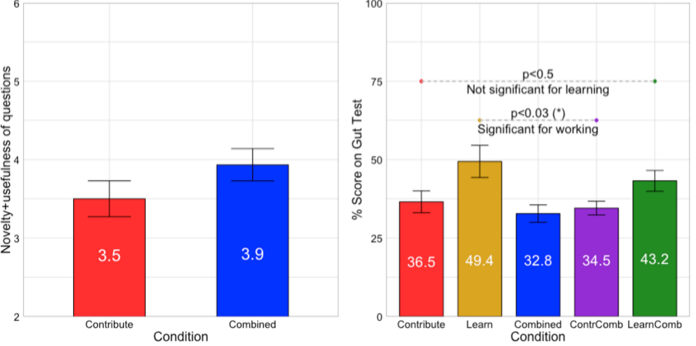
\includegraphics[width=1.0\textwidth]{figures/gutinstinct/gi-7.png}
%  \caption[Results: Question quality, Learning Score, and Time Spent]
%{a) Participants in Contribute and Combined conditions created questions of similar quality b) Participants in Learn condition performed the best on a summative test. Learning did not show a significant effect on score but working did c) There were no significant differences in time spent in lab session across the conditions \index{gi-7}}
%  \label{fig:gi-7}
%\end{figure}

\begin{figure}[h] 
  \centering
  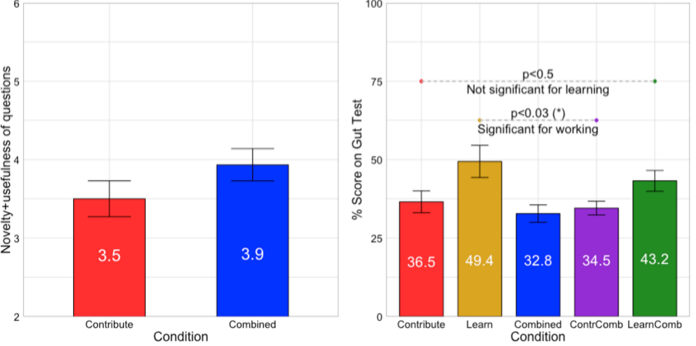
\includegraphics[width=1.0\textwidth]{figures/gutinstinct/gi-7.png}
  \caption[Results: Question quality and learning score]
{a) Participants in Contribute and Combined conditions created questions of similar quality b) Participants in Learn condition performed the best on a summative test. Learning did not show a significant effect on score but working did \index{gi-7}}
  \label{fig:gi-7}
\end{figure}

\textit{Work}: Did access to Coursera learning material (Combined) impact quantity and quality of questions relative to not having access (Contribute)? The Combined participants generated questions of similar novelty and usefulness (M = 3.5) as Contribute participants (M = 3.93), Mann–Whitney U = 79, n1 = 14, n2 = 15, p $<$ 0.23 two-tailed (Figure~\ref{fig:gi-7}a). Figure~\ref{fig:gi-8} shows two examples of questions rated by experts. Ten of the 29 questions mirrored questions found on the American Gut survey. Half of the participants’ questions (14 of 29) asked about diet. Participants in Combined and Contribute conditions generated a total of 14 and 15 questions, respectively, averaging one question per participant (see Figure~\ref{fig:gi-9}). 

\begin{figure}[h] 
  \centering
  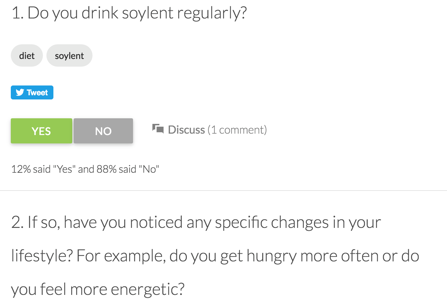
\includegraphics[width=0.48\textwidth]{figures/gutinstinct/gi-8a.png}
  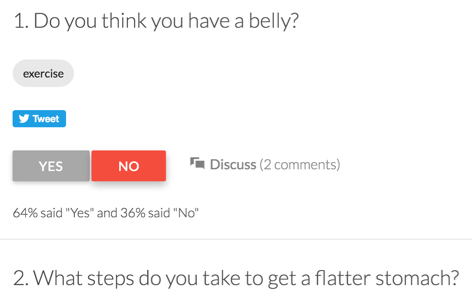
\includegraphics[width=0.48\textwidth]{figures/gutinstinct/gi-8b.png}
  \caption[Examples of questions added by participants]
{An example of a good and bad question added by participants. Soylent question was scored 5/6 (2 on novelty and 3 on usefulness) while the belly question was rated 2/6 (1 on novelty and 1 on usefulness) \index{gi-8}}
  \label{fig:gi-8}
\end{figure}

\textit{Learning}: Did participants instructed to ask questions (Contribute \& Combined) score differently than those who were not (Learning)? Did access to learning videos (Learning \& Combined conditions) impact quiz scores relative to not having access (Contribute)? A two-factor ANOVA estimated these effects, finding significantly lower scores for those requested to ask questions. By contrast, access to learning materials did not yield a significant difference in quiz score.

The Learn participants performed scored higher (M = 5.93) on Learning test than participants in Combined (M = 4.38) or Contribute (M = 3.93) conditions. An analysis of variance showed that this effect was significant for working, F(1, 39) = 5.22, p $<$ 0.03, but not for learning, F(1, 39) = 0.46, p $<$ 0.5 (Figure~\ref{fig:gi-7}b). The effect size for working was small (Cohen’s effect size d = .11).

\begin{figure}[h] 
  \centering
  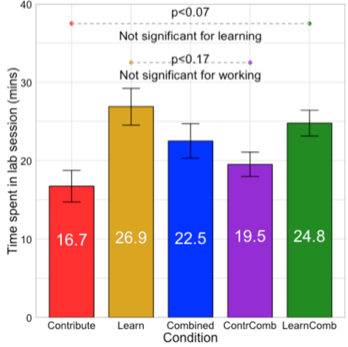
\includegraphics[width=0.5\textwidth]{figures/gutinstinct/gi-7-1.png}
  \caption[Results: Time spent]
{There were no significant differences in time spent in lab session across the conditions \index{gi-7-1}}
  \label{fig:gi-7-1}
\end{figure}

\textit{Engagement}: The mean length of lab session was ~20 min (varying from 9-40 min). Learn participants spent marginally more time (M = 26.9 min) in the lab session than participants in Combined (M = 22.5 min) or Contribute (M = 16.7 min) conditions. An analysis of variance showed that this effect wasn’t significant for either Learning F(1, 41) = 3.40, p $<$ 0.07 or working F(1, 41) = 1.95, p $<$ 0.17, (Figure~\ref{fig:gi-7-1}). Combined and Contribute participants contributed 35 discussion comments each; Learn participants contributed 10 discussion comments.

38 of 40 correspondents reported prior use of online courses, varying from occasional use of online learning material to taking more than five online classes. Preliminary analyses found no effects for gender and nationality (Indian or non-Indian), so these were excluded from further analyses. Table~\ref{tab:gi-results1} summarizes results from the experiment. 

%%%% TABLE 2 %%%%
\vspace{0.25in}
\begin{table}[!ht]
\caption[Summary of results from experiment]{Summary of results from experiment}

\vspace{-0.25in}
\begin{center}
%\setlength{\tabcolsep}{10pt} % Default value: 6pt
\renewcommand{\arraystretch}{1.5} % Default value: 1
%\begin{tabular}{|p{1in}|p{1in}|p{1in}|p{1in}|p{1in}|}
\begin{tabular}{p{1in}p{1in}p{1in}p{1in}p{1.5in}}
\hline
\textit{Measures (mean values)}	& \textit{Combined} &	\textit{Contribute}	& \textit{Learn}	& {\it p} \\
%\multicolumn{5}{|l|}{\bf No difference in quality or quantity of questions across Combined or Contribute}   \\
\multicolumn{5}{l}{\bf No difference in quality or quantity of questions across Combined or Contribute}   \\
Quality of questions (2-6 scale)  &	3.5 &	3.93	&-	& $<$ .23\\
\# of questions/\# of participants &	14/14 &	15/15 &	- &	-\\
%\multicolumn{2}{|l|}{\bf  Working reduced test scores}  & & & \\
\multicolumn{2}{l}{\bf  Working reduced test scores}  & & & \\
Test score (max: 12 pts) & 4.38	& 3.93 & 5.92 & L $<$ .5, W $<$ .03 \\
%\multicolumn{5}{|l|}{\bf Learning or contributing did not have a significant effect on time spent in lab }   \\
\multicolumn{5}{l}{\bf Learning or contributing did not have a significant effect on time spent in lab }   \\
Time taken in lab session (min) & 22.5 & 16.7 & 26.8 & L $<$ .07, W $<$ .17\\
\# of discussion comments & 35 & 35 & 10 & - \\
\hline
\end{tabular}
\end{center}
\label{tab:gi-results1}
\end{table}

\begin{figure}[h] 
  \centering
  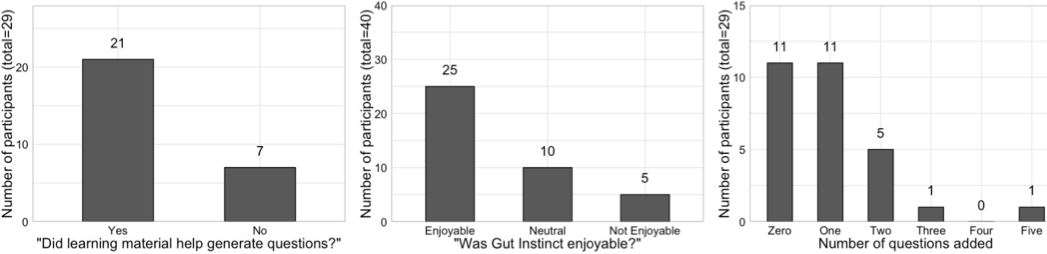
\includegraphics[width=1.0\textwidth]{figures/gutinstinct/gi-9.png}
  \caption[Participants' self-reports]
{Most participants reported that the learning experience was helpful and the system was enjoyable. 65\% of participants asked questions; the mode was 1) \index{gi-9}}
  \label{fig:gi-9}
\end{figure}

%%%%%%%%%%%%%%%%%%%%%%%%%%%%%%%%%
\section{Discussion}
These results suggest that some learners create useful research questions based on their lifestyle but its effect on better learning is unclear.

\textit{Why did Learn participants perform better on tests?}
Learn participants had a clear objective: learn about the gut microbiome, practice problems related to it, and take a summative test. By contrast, participants in the other two conditions had to both generate novel questions and take the summative test. They may have placed less emphasis on the test. Generating questions and taking test on a novel topic might have required greater effort than what the participants wanted to put in. Additionally, difficulty of creating questions may have lowered participants’ confidence in taking the test. 

\textit{Personalized learning and need for feedback}
Participants were curious to know the microbiome science behind disclosed aspects of their lifestyle. One participant commented, “After answering the question, I would expect to see some succinct information about where my lifestyle stands with respect to scientific wisdom.” Participants also asked for a section curated for them by the tool, or a section where they could save items of personal relevance.
 
\textit{Need for self-directed learning}
Online learning material provided useful information about a complex topic like the microbiome hoping that it might spur participants to find and use other similarly trustworthy sources of their liking. In the lab, participants used web search to find relevant resources. Most participants reported that they did not search at home. 

\textit{Learning did not improve quality of work}
Combined participants did not generate questions of higher quality than those without learning material (Contribute condition). Crowdclass~\cite{Lee2016} found similar results where workers who simply classified images did better than those who learned about decision trees and subsequently classified images as an assignment. How do online learning materials and useful work tie to each other? Gut Instinct explored one design point where learning and working were provided specific components in the tool to reduce participant confusion. An alternate approach could be to have a work-biased design where learning material would be tailored to participants’ questions or a learn-biased design where participants could add questions only in the specific context of learning materials. For instance, people could raise questions at different point of a topic video~\cite{Lee2015b} rather than using a separate part of the tool.
 
\textit{Difficulty of generating questions}
A remarkable and concrete measure of participants’ insights is that ten of their questions mirrored those asked by the American Gut survey~\cite{KnightLab2016}. Unsurprisingly, other participants reported difficulty creating good questions. Asking questions is a valuable metacognitive experience that can be scaffolded by examples of good questions from experts. 

Gut Instinct sent email asking people to contribute, reminding them of the importance of their task, and showing successful examples of citizen science work. Such reminders 
prompted a temporary increase in questions increased or discussion contributions~\cite{Kotturi2015} but did not lead to a sustained stream of questions and discussions. Some participants complied with the letter of the request but not the spirit by taking a sample question and tweaking it slightly.

\textit{What kind of innovation can we expect from citizen science}
Half of participants’ questions were about diet. Diet offers both a clear influence mechanism and immediate personal relevance. While a compelling video about effect of diet on the microbiome likely helped, a video alone appears insufficient: for instance, the topic of genetics also had a video, but no participants asked questions about genetics. Moreover, many diet questions are perceived as less personally disclosive than genetics questions.
 
That participants asked many questions about diet and none about genetics is consistent with patterns of where lead users innovate, and where they don’t~\cite{VonHippel2005a}. Lead-user innovation works best for \textit{need intensive} problems where people’s lived experiences provide the key ingredient, e.g., a snowboarder who cuts their boots to improve fit. These innovations arise through trial and error, and solution efficacy is readily observable. Lead-user innovation is less common with \textit{solution intensive} problems, where highly technical knowledge, access to equipment, and/or significant financial capital are critical. 
 
\textit{Does browsing displace contributing?}
Participants spent most of the lab session browsing discussions and learning material. By our observation, later participants spent more time using the system in the lab. Despite spending more time browsing discussions, we think later participants added fewer questions. Participants mentioned that browsing and answering questions felt like \textit{contributing} without putting in a lot of effort. Participants also reported that they had to break a mental barrier to publicly post a discussion comment or question. 

\subsection*{Limitations}
Participants could login as little or as many times as they wished. One participant commented that even though she had some ideas to add, she was conscious of disclosing information about her personal life (participants were anonymous). It may be that using the tool in an experiment made them more cautious of what they added or commented.
As a web application, participants assumed comparable facilities to forum/ discussion sites like Quora. This exemplifies a challenge of testing research prototypes: the absence of production-level features can change participants’ impressions and possibly their behavior.

%%%%%%%%%%%%%%%%%%%%%%%%%%%%%%%%%%%%
\section{Science with Learners: Promise \& Challenges}
This chapter investigated the merits of combining learning and contributing. While experimental results did not show the hypothesized additive benefits, we still believe this combination has potential. Is it intrinsically self-contradictory to ask learners to contribute scientific ideas? Not necessarily. In addition to the diversity benefits that the global community brings, those with brand new knowledge can, for example, give useful feedback to peers~\cite{Kulkarni2013peer}. Furthermore, the newly-aware sometimes articulate useful insights that familiarity has blinded experts to~\cite{Hinds1999}. Drawing on the results, related literature, and our intuitions, here are avenues that might find additive benefits where this experiment did not.

\textit{Aligning objectives}
The chapter’s experiment gave participants two objectives: take a summative test and generate ideas for lifestyle-microbiome relationships. While both relate to the same general topic---the microbiome---the “doing” of each was quite different. For example, the question that the fewest participants answered correctly asked which type of bacteria population would be affected by a behavior change. While the test emphasized specific biological facts like this, participants’ GutBoard questions were much more general. Consequently, it is not surprising that success on one didn’t catalyze success on the other. Conversely, given the mild negative correlation, it seems likely that time spent on one might have taken away from time spent on the other. More tightly aligning the test of learning with the work activities could yield the additive benefits we seek. (We say \textit{test of learning} because participants may indeed have learned more in ways not measured.) 

We also hypothesize that an additive benefit is more likely when the knowledge and/or motivation generated by one activity transfers to the other. While this may seem obvious in retrospect, the loose-connection problem observed here may be relatively common. We hope the results warn against this risk.

\textit{Make learning \& work personally relevant}
Many American Gut Project (AGP) participants exhibit a strong intrinsic motivation to learn more about why they have a particular microbiome~\cite{Debelius2016}. The students who participated in this experiment may not have equivalently strong motivation. Motivated users may increase the quality of citizen science work. For instance, AGP participants could organize a focused effort around a specific health issue like Type 1 diabetes or Inflammatory Bowel Disease (IBD). Similar to how Wikipedia editors co-ordinate efforts~\cite{Krieger2009} using Gut Instinct with more differentiated roles like question generation, question ranking, and literature search might lead to further distinguishing work.

\textit{Learning \& working: integrate \& provide clear criteria}
We believe that integrating learning and work will be mutually beneficial when learning new material immediately opens up the possibility of contributing useful work and contribution solicitations include relevant learning material. This extends problem-based learning~\cite{Savery1995} and just in time learning~\cite{Bolton1999} to the scale of Internet. For example, browsing StackOverflow before fixing programming questions leads to better work, and lateral learning~\cite{Mamykina2011}. Similarly, global-scale distributed contributions like peer review have enabled massive online courses to offer creative, open-ended assignments through peer review~\cite{Kulkarni2013peer}. Such active learning approaches seek a dual objective of content learning and metacognitive growth~\cite{Crouch2001}.
 
Reflection and curiosity play a similar orienting role: having people guess the answer to a task-relevant question before performing the main task led to better performance on the task when hints were revealed to maintain the curiosity of the learners~\cite{Aleven2006, Law2016a}. Similarly, the surprise that arises from making a guess that’s revealed to be wrong generates a \textit{teachable moment} for learners. How might we use these lessons for online learners to teach themselves about specific domains while performing useful work? 

\textit{Other fields for this approach}
Many other fields may benefit from the diverse contexts that online citizen scientists offer. For example, 96\% of psychology experiments used participants from Western industrialized countries~\cite{Henrich2010a}. Recent attempts have started to collect and analyze data about people all across the world by offering them fun-based rewards in lieu of collecting data about their online interactions~\cite{Reinecke2015}. Success of such initiatives hints at a motivated set of online participants who could also benefit from learning about cultural psychology concepts in more depth while undertaking relevant scientific work. 


This chapter investigated techniques for integrating learning and citizen science for the benefit of both. For us, the most striking result is that users contributed many causal questions of sufficient novelty and importance that they only recently have emerged in the literature. It is possible that other of the causal questions will be borne out in the future. This study also illustrates the challenges of double-bottom-line work. Specifically, these dual objectives can be in tension rather than being additive. The chapter describes the Gut Instinct system and suggests strategies that may help the dual objectives enhance each other. Looking forward, we hope the approach introduced here will find value in other domains especially where the science is nascent and/or contextual information is key. The knowledge of science impacts a diverse planet; in the future, this diverse community may importantly contribute to it.


This chapter, in part, includes portions of material as it appears in \emph{Gut Instinct: Creating Scientific Theories with Online Learners} by Vineet Pandey, Amnon Amir, Justine W. Debelius, Embriette R. Hyde, Tomasz Kosciolek, Rob Knight, and Scott R. Klemmer in the proceedings of the ACM Conference on Human Factors in Computing Systems (CHI 2017). The dissertation author was the primary investigator and author of this paper.

\chapter{Collaboratively generating hypotheses}
\begin{figure}[h] 
  \centering
  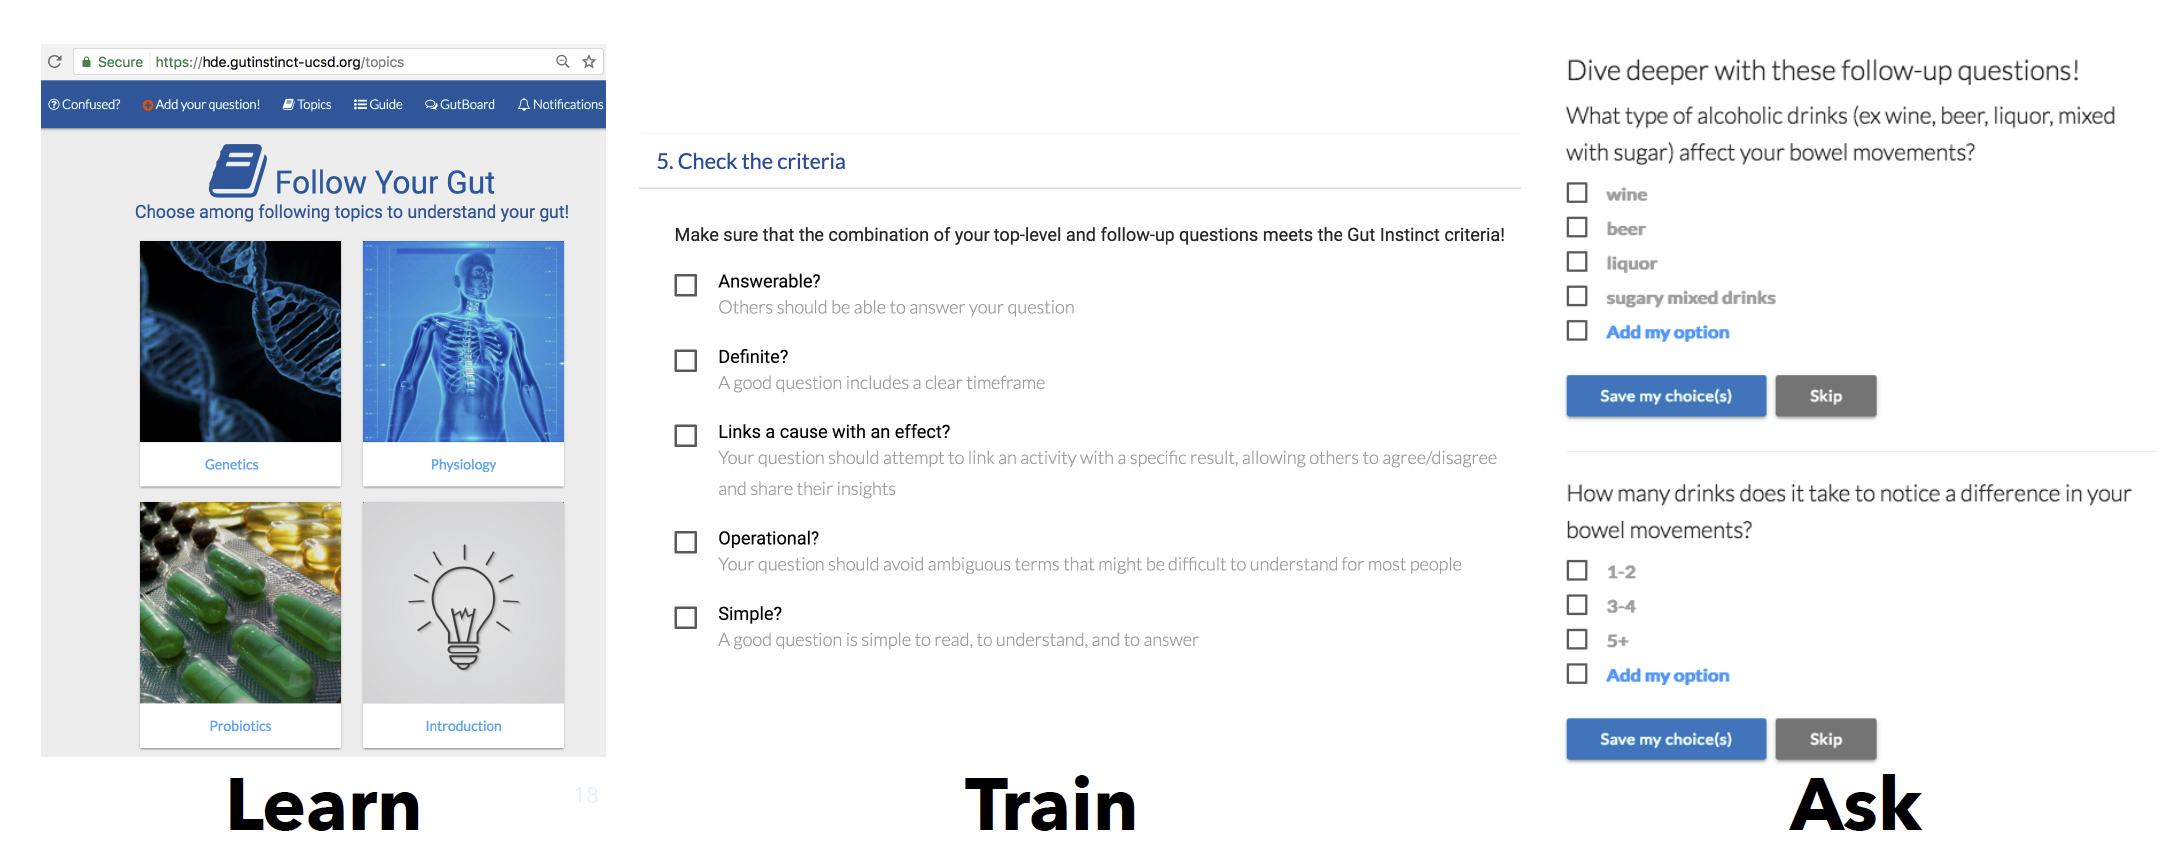
\includegraphics[width=1.0\textwidth]{figures/docent/fig-0.png}
  \caption[The Docent Learn-Train-Ask workflow]
{The Docent Learn-Train-Ask workflow.\index{docent-0}}
  \label{fig:docent-0}
\end{figure}

\textit{People’s lived experiences provide intuitions about health.
Can they transform these personal intuitions into testable hypotheses
that could inform both science and their lives? This
paper introduces an online learning architecture and provides
system principles for people to brainstorm causal scientific
theories. We describe the Learn-Train-Ask workflow that
guides participants through learning domain-specific content,
process training to frame their intuitions as hypotheses,
and collaborating with anonymous peers to brainstorm related
questions. 344 voluntary online participants from 27
countries created 399 personally-relevant questions about the
human microbiome over 4 months, 75 (19\%) of which microbiome
experts found potentially scientifically novel. Participants
with access to process training generated
hypotheses of better quality. Access to learning materials improved
the questions’ microbiome-specific knowledge.
These results highlight the promise of performing personally 
meaningful scientific work using massive online learning
systems}

%%%%%%%%%%%%%
\section{NEEDS A SUBSECTION HERE}
Thinking like a scientist involves generating useful questions,
operationalizing them as hypotheses, and testing them
with experiments. While people generate (implicit) intuitions
from lived experiences, transforming tacit knowledge into
explicit questions is not easy. People don’t always realize the
extent of their knowledge and even when they do, asking questions 
that can be answered by others to yield clear, actionable
insights is hard. For instance, people often bury
questions in long entries (Figure~\ref{fig:docent_1}. Transforming intuitions
into falsifiable questions is a key skill for scientists and designers
alike. How can people create questions that are novel
(contain new information), useful (relate to and potentially
extend existing scientific knowledge), easy to answer, and
specific (relate to only one topic)? Such questions can
potentially accelerate research in nascent scientific domains,
such as the human microbiome.

This paper contributes (1) the Learn-Train-Ask method for
people to perform personally meaningful scientific work by
sharing personal insights and receiving feedback from
others, and (2) its embodiment in Docent — a novel
crowdsourcing system for causal scientific questions. Docent
enables novices to ask useful questions by learning domainspecific
content, undergoing process training to develop
task-specific skills, and collaborating with online peers. A
between-subjects study evaluated this new method by measuring
the quality of participants’ questions to test causal scientific
theories about the human microbiome. 344 voluntary
online participants from 27 countries — including participants
from the American Gut Project, Open Humans,
Coursera, and Reddit — signed up to share personally-relevant
questions about the human microbiome. Participants
created 399 questions, 75 (19\%) of which microbiome experts
found novel. Participants with access to process training
generated hypotheses of better quality. Access to
learning materials improved the questions’ microbiome-specific
knowledge. These results highlight the promise of performing
personally-meaningful scientific work using
massive online learning systems.


%\begin{figure}[h] 
%  \centering
%  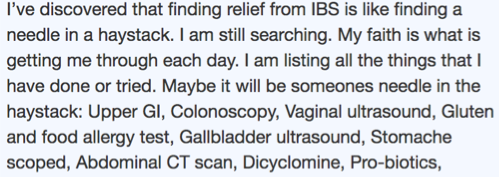
\includegraphics[width=1.0\textwidth]{figures/docent/fig-1.png}
%  \caption[]
%{This post to a Mayo Clinic forum shows how people
%seeking advice online combine many ideas into one post..\index{docent-1}}
%  \label{fig:docent-1}
%\end{figure}

\begin{wrapfigure}{r}{0.5\textwidth}
  \centering
  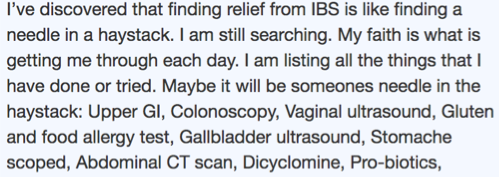
\includegraphics[width=0.5\textwidth]{figures/docent/fig-1.png}
  \caption[Post to a Mayo Clinic forum]
{This post to a Mayo Clinic forum shows how people
seeking advice online combine many ideas into one post..\index{docent-1}}
  \label{fig:docent-1}
\end{wrapfigure}

%%%%%%%%%%%%%%%%%%%%%%%%%%%%%%%%%%%%%%%%%%%%%%%%%%%%%%%%%%%%%
\section{The Docent Social Computing System}
The Docent social computing system enables people to create specific, personal hypotheses by providing: content learning \& process training; a guided question-asking interface; and an online collaboration platform. Docent was designed via multiple iterations of early pilot studies. Docent’s pilot participants were ~50 lead users of the American Gut Project \& Health Data Exploration workshop (hdexplore.calit2.net). Early participants used the website to provide in-person feedback about the interface. As the sys-tem matured, later participants provided both explicit online \& in-person feedback along with usage data that led to a number of improvements. For instance, a pilot session led to the idea to enable editing others’ questions to improve clarity (especially for non-native English speakers).

The Docent web application is built with Meteor (meteor.com), and extends Gut Instinct~\cite{Pandey2017} that also leverages learning materials, but does not address causal theory generation. The front-end uses BlazeJS (blazejs.org) and is styled with Materialize (materialize.css).

\subsection{Learn-Train-Ask: From Intuitions to Hypotheses}
Docent embodies three main principles. The first is two-way integration of learning and asking questions for improved conceptual understanding of the microbiome. Novel, domain-specific work (such as asking questions for micro-biome discovery) needs to integrate a novel idea with existing knowledge, perhaps even using specific terms/metrics in the process (e.g. Bristol stool scale for quality of bowel movement). To forge a two-way link between learning and asking questions, Docent provides online lectures and feed-back on the questions people create using scientific material. For instance, for a question about the effects of probiotics on mood among people suffering from gastrointestinal diseases, Docent would provide feedback using lectures about probiotics, gastrointestinal diseases, and the gut-brain axis.
The two attributes that training questions seek to model are a) that others can answer them, and b) that each addresses a single topic. Training helps participants get a feel for how precise questions should be: overly vague and overly specific terms both reduce a question’s utility. To link many ideas with one cause, a sequence of questions can iteratively refine a hypothesis space. For instance, a question linking probiotics use to bowel movements might begin by asking how frequently people consume probiotics and in which form, following up by asking about bowel movements.
Third, Docent provides clear success criteria: creating useful questions. Docent converts question-asking and answering into an engaging social interaction by enabling people to participate in multiple ways, such as by asking questions, adding follow-ups, editing questions to improve clarity, or responding to questions. A new user can access the entire Docent system only after adding a question.

\begin{wrapfigure}{r}{0.5\textwidth}
  \centering
  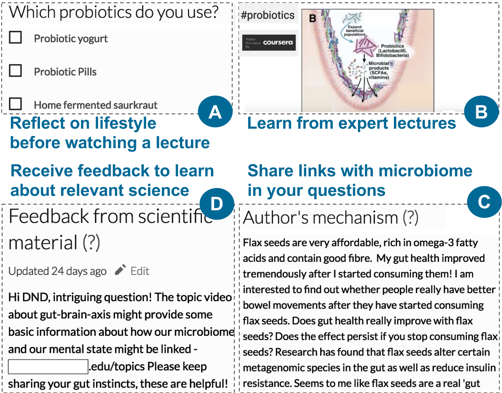
\includegraphics[width=0.5\textwidth]{figures/docent/fig-2.png}
  \caption[User flow of Docent learning module]
{User flow of Docent learning module. Participants reflect on their lifestyle by (A) answering a personal question before (B) watching an online lecture about probiotics and the microbiome. Participants (C) must propose a mechanism when adding a question and (D) they receive feedback from scientific material on their questions. Probiotics was one of 16 topics for which Docent provided ~5min long expert lectures.\index{docent-2}}
  \label{fig:docent-2}
\end{wrapfigure}
 
\subsection{Learn content: Integrate Concepts with Insights}
Docent’s learn module teaches people about the gut microbiome using online lectures, lifestyle questions, feedback from scientific material on questions, and guessing potential mechanisms (Figure~\ref{fig:docent-2}). We describe each below. 

%\begin{figure}[h] 
%  \centering
%  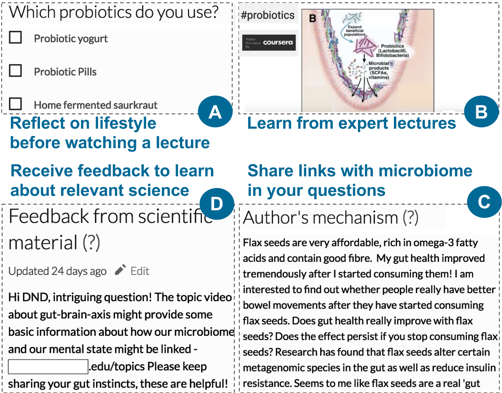
\includegraphics[width=1.0\textwidth]{figures/docent/fig-2.png}
%  \caption[User flow of Docent learning module]
%{User flow of Docent learning module. Participants reflect on their lifestyle by (A) answering a personal question before (B) watching an online lecture about probiotics and the microbiome. Participants (C) must propose a mechanism when adding a question and (D) they receive feedback from scientific material on their questions. Probiotics was one of 16 topics for which Docent provided ~5min long expert lectures.\index{docent-2}}
%  \label{fig:docent-2}
%\end{figure}

Online lectures to improve conceptual understanding: The human microbiome is nascent, yet fast-growing. There is a lot of room for new contributions, but few people have up-to-date and accurate knowledge, even to the extent that it exists. People ask more questions when the learning material causes inconsistencies in their understanding of a topic~\cite{Miyake1979a}. Since few people know about the microbiome, Docent uses introductory learning material curated from Gut Check, a Coursera MOOC ~\cite{Knight2016}, rather than scientific papers that may be too abstruse. Apart from introductory material about the microbiome, Docent also provides learning material about specialized topics, such as gastrointestinal diseases \& the gut-brain axis, to engage people in guided discovery learning based on their interests and health conditions (Figure~\ref{fig:docent-2}B).

 Personal questions to improve reflection: Prompting participants to explicitly reflect on the learning topic can increase curiosity and question-quality~\cite{Aleven2006, Law2016}. Before watching a lecture about the microbiome, Docent invites people to answer questions that make them reflect on the connection between the learning material and their lifestyle (Figure~\ref{fig:docent-2}A).

Guessing a mechanism to reflect on question and knowledge: Docent asks people to guess mechanistic explanations for how the microbiome can play a role in answering their questions (Figure~\ref{fig:docent-2}C). This is intended to help users learn by connecting personal observations with existing knowledge~\cite{Simon2004}.

Feedback from scientific material: Rapid, relevant feedback improves quality~\cite{Hattie2007}. The first author provided links to scientific papers and web content in response to people’s questions. To integrate questions with Docent’s learning material, they also received feedback on their questions using links to the Coursera MOOC lecture hosted on Docent (Figure~\ref{fig:docent-2}D). Participants also added scientific papers to questions. 

\subsection{Process training: From Intuitions to Scientific Questions}
Docent uses three components to help people ask useful questions: a training guide, expert examples, and a question-asking checklist (Figure~\ref{fig:docent-3}). 

\begin{figure}[b] 
  \centering
  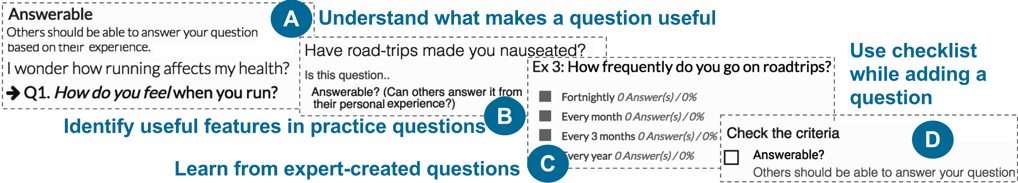
\includegraphics[width=1.0\textwidth]{figures/docent/fig-3.png}
  \caption[The Docent training process]
{The Docent training process. People (A) learn what makes a question useful, (B) practice on sample questions, and (C) read expert-curated questions. (D) When asking a question, a checklist reminds people to ensure their question meets the criteria for useful questions. Answerability was one of 5 features for which Docent provided training.\index{docent-3}}
  \label{fig:docent-3}
\end{figure}

Training guide to identify useful features: New Docent participants must add a question before accessing the entire system (learning, training, and the GutBoard). Before asking a second question, however, a user needs to complete the training guide: people learn about five features of successful questions; train by identifying these features in two sample questions (Figure~\ref{fig:docent-3}A,B); and then immediately ask a question. Training draws on successful techniques from crowd work and peer assessment by using gold standards~\cite{Kittur2013} and rubrics~\cite{Andrade2005}. When adding a question, a checklist reminds participants about the features of good questions (Figure~\ref{fig:docent-3}D).

\subsection{Ask well-framed questions }
Good questions specify a cause and associated effects.

\textit{Two-step question format to separate cause and effect}: Docent questions comprise two parts: a top-level question identifies a cause (e.g., frequency of consuming probiotics). A follow-up question links the cause to a specific insight from the user (e.g., effects of consuming probiotics). The creator can add multiple follow-ups to link a cause to many effects.

\textit{Templated options to reduce common errors}: Poor and/or vague options can discourage responses, erode esprit de corps, and model bad behavior that others follow. To counter this, Docent provides popular templated multiple-choice options. These templates are editable, but providing templates helps people be specific.

\textit{Cues to improve question quality}: These cues comprise alert messages when people add long or short options; notes about details needed in their questions; and restricting people from adding a question without providing a potential mechanism or comment.

\subsection{GutBoard: Crowd responses, Discussion, Expert feedback}
The GutBoard is designed for quick question traversal, easy response, and collaboration. Only the top-level question from each question is displayed: if a user is not interested in, say probiotics, they can simply skip that set. However, to access follow-ups, people need to answer the top-level question by selecting from the existing options or adding their own. To focus people’s attention on specific questions, the first author starred promising questions that people can access from the Starred tab (Figure~\ref{fig:docent-4}). Starring signifies that a question is likely of high quality or broad interest, and helps focus participants’ answering efforts on them. Docent also enables people to bookmark questions of interest, so they can visit them again. 

To de-incentivize lurking and increase engagement, the GutBoard shows only one question at a time; we call this sequential access. When people could see multiple questions simultaneously (parallel access), they skimmed through many questions without interacting with them. 

\begin{wrapfigure}{r}{0.5\textwidth}
  \centering
  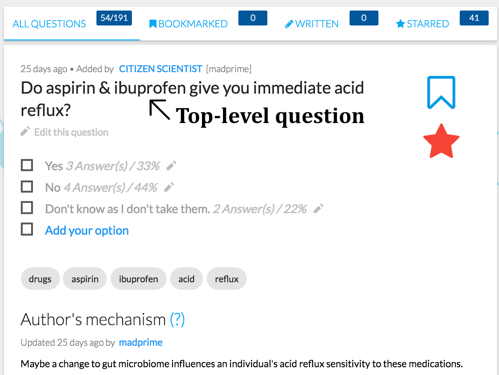
\includegraphics[width=0.5\textwidth]{figures/docent/fig-4.png}
  \caption[Participants can see follow-up questions, add new options, new follow-up questions, edit the question, guess potential mechanisms, and bookmark]
{After answering a top-level question, participants can see follow-up questions, add new options, new follow-up questions, edit the question, guess potential mechanisms, and bookmark. A star (added by an expert) shows that this question may be promising for further enquiry by people.\index{docent-4}}
  \label{fig:docent-4}
\end{wrapfigure}

%%%%%%%%%%%%%%%%%%%%%%%%%%%%%%%%%%%%%%
\section{Hypotheses: Effect of Learning and Training on Question Quality}
Learn-Train-Ask scaffolds collaborative scientific question generation. We tested the following hypotheses in the context of brainstorming potential causal relationships in the human gut microbiome.

\textbf{H1. Access to learning improves question’s content.}
While people’s questions are based on their experiences and curiosity, aligning them with what is already known about the microbiome can uncover novel insights. Alternately, learning can make people reflect less on their personal knowledge and more on institutional knowledge, reducing the novelty of their questions. A question is deemed to have good content if it is insightful (exhibits microbiome-specific knowledge) and novel (contains potentially new knowledge for microbiome science).

\textbf{H2. Just-in-time training improves question’s structure.}
We hypothesize that training helps people create useful questions for receiving feedback as well as for generating insights for researchers. A question is deemed to have good structure if it is easy for other participants to answer and focuses on one topic.

\section{Study: Scaffolds for Better Questions}
A between-subjects study compared the participants’ question quality across four conditions: Learn, Train, Neither and Both. In the Learn condition, participants saw online lectures, answered personal questions, guessed mechanisms, and received feedback from scientific material on their questions (provided by the first author). The Train condition provided participants access to a training guide, expert examples, and checklist. In the Neither condition, participants did not have access to either the Learn or Train step, while in the Both condition they had access to both. All participants had access to the question-asking and GutBoard collaboration module (with required condition-appropriate adjustments — e.g., participants in Learn and Both conditions were asked to guess the mechanism for their question, while participants in the other two conditions were asked to add a discussion comment). The GutBoard content was unique to the participants for a specific condition, to ensure that participants were not influenced by behavior in other conditions. 

\subsection*{Method}
Participants were randomly assigned to one of the four conditions. Each gave participants access to a condition-specific Docent. Each condition began with an introductory tour describing the significance of microbiome research and the importance of their contributions towards making discoveries. At the end of the tour, participants in every condition had to add one question (using identical question-asking modules) before moving on. Docent sent regular email reminders about site activity. 

\subsection*{Participants}
Recruitment: Participants were recruited via online publicity. To invite people especially interested in their microbiome, the American Gut Project emailed 550 participants. Docent was promoted on the American Gut Project’s and their collaborators’ Facebook and Twitter pages. Docent was added as a project on Open Humans (openhumans.org) — a platform where people donate their personal data for scientific research and participate in scientific experiments. Docent was posted on multiple subreddits pertaining to health and lifestyle (e.g., reddit.com/r/keto) and added as an optional assignment to the Gut Check Coursera MOOC~\cite{Knight2016}. Participation was voluntary and unpaid; participants were entered in a raffle for an American Gut Microbiome kit (provided for \$99 on American Gut’s crowdfunding page (fundrazr.com/campaigns/4Tqx5)) on survey completion.

\subsection*{Measures}
Dependent variables comprised structure, content, and creativity of questions (Table 1). American Gut researchers with multiple years of post-PhD expertise independently rated all 399 questions. (330 questions were rated by three; 69 were rated by two). The average ICC measure for 3 raters was 0.48 with 95\% CI[0.42,0.54], (F (328,656) = 3.73, p$<$.001). Raters agreed that evaluating novelty was difficult since the nascent microbiome literature is rapidly growing.

Raters were instructed to assign points for structure if it asked participants about a specific topic that they could answer. For example, “How often do you consume fermented foods?” was rated as both answerable by participants and specific, while, “Does our modern agricultural system affect our microbiome?” was neither answerable nor specific. Question content was the sum of insightfulness and novelty. Insightfulness addressed the quality of the microbiome content in the questions. Novelty was assessed as the potential to create new knowledge in the microbiome field and operationalized as the lack of research papers about the specific question. For example, “Does consuming bone broth improve digestion?” was rated as both insightful and novel, while, “Can microbiome cure cancer?” was neither insightful nor novel. Broad questions related to well-studied topics or those fishing for links with the microbiome, such as the difference between generic vegetarian and meat-based diet were not deemed novel. A question was considered creative if it suggested an interesting idea without necessarily drawing it from personal experience. 

\subsection*{Results}
344 participants completed the baseline exercise, continuing to the condition-specific intervention (Learn, Train, Both, or Neither). Participants who asked follow-on questions were scored as described above; those who did not were scored as 0. Table 2 shows, for each condition, the total number of participants, the number that provided questions, the total question points, and the average score across all participants. The overall quality of the questions generated in the combined Train+Learn condition is the highest (0.56 points) and appears to stand out from the others. We used a permutation test (a kind of bootstrapping method) to assess the statistical reliability of this apparent interaction, namely, whether the combined Learn-Train condition produces better questions than is expected from the independent main effects of the Learn and Train conditions. Indeed, a permutation test with 10,000 replications found that the observed differences in question points are different than the expected differences (generated by the main-effect marginals) as they fall outside the 95\% confidence interval [-24.5, 24.5], p$ <$.05. The three score components (structure, content, and creativity) were pairwise weakly correlated (r=0.32, p$ <$ 0.02; r=0.19, p$ <$ 0.17; r=0.33, p$ <$ 0.01). 

\begin{figure}[h] 
  \centering
  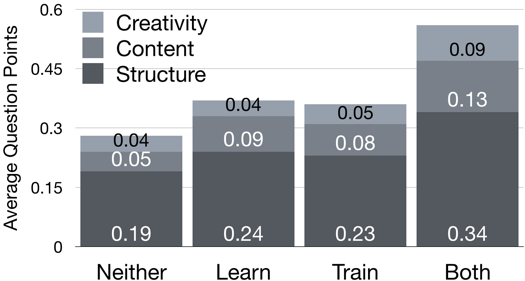
\includegraphics[width=1.0\textwidth]{figures/docent/fig-5.png}
  \caption[Training improved the overall question quality but learning did not]
{Training improved the overall question quality (p <.05) but learning did not (p $<$ 0.1). H1: Training marginally improved question structure (p <.06). H2: Learning improved question content (p <.05).\index{docent-5}}
  \label{fig:docent-5}
\end{figure}

\textit{Total question points}: Training improved overall question quality (M=0.31, vs. M=0.47); a permutation test with 10,000 replications found that the observed difference in question points are different than the expected differences as they fell outside the 95\% CI[-19.5, 19.5], p <.05. Learning did not improve overall question quality (M=0.32, vs. M=0.46); a permutation test with 10,000 replications found that the observed differences in question points are not different than the expected differences as they did not fall outside the 95\% CI[-29.5, 29.5], p < 0.1. (Figure~\ref{fig:docent-5})

\textit{Structure}: H1: Did access to training material (Train and Both conditions) improve the structure of questions relative to not having access (Learn and Neither conditions)? Training marginally improved question structure (M=0.21, vs. M=0.29); a permutation test with 10,000 replications found that the observed difference in question structure points are different than the expected differences as they did not fall outside the 95\% CI[-9.5, 9.5], p <.06.

\textit{Content}: H2: Did learning material (Learn and Both conditions) improve the content of questions relative to not having access (Train and Neither conditions)? Learning improved question content (M=0.06, vs. M=0.11); a permutation test with 10,000 replications found that the observed difference in question content points fell outside the 95\% CI[-9, 9], p <.05.

\textit{Creativity}: Did training or learning material (Learn and Both conditions) impact the creativity score of questions relative to not having access (Train and Neither conditions)? Neither training (M=0.04 vs. M=0.07; 10,000-replication permutation test 95\% CI[-4, 4], p < 0.08) nor learning (M=0.05 vs. M=0.07; 10,000-replication permutation test 95\% CI[-4, 4], p < 0.2) improved the creativity score.

%%%%%%%%%%%%%%%%%%%%%%%%%%%%%%%
\section{Discussion}
\subsection{The effect of learning and training on questions}
As a check of random assignment, participants’ required pre-intervention question was of comparable quality in all conditions. Participants in the Both condition scored higher total question points after the intervention. Training en-forced a tutorial when asking a question, and the add-question module presented heuristics for asking better ques-tions. This tight integration may have enabled people to focus their questions on a specific topic and frame their questions to be answerable by others. Moreover, the pres-ence of learning material might have provided a useful setup and improved participant engagement leading to greater number of questions, and question points.

The study found a significant effect for learning on content ratings and a marginally significant effect for training on structure ratings. This asymmetry could be substantive: that learning improves content, but training only lightly improves structure. Alternatively, it could be a statistical mi-rage: the lower inter-rater reliability for content might show an effect if there isn’t one. Inter-rater reliability was higher for structure (M=0.65; 95\% CI[0.59,0.69] (F (328,656) = 6.59, p < .001)) than content (M = 0.11; 95\% CI[0.04,0.18], (F (328,656) = 1.37, p <.001)).
We hypothesize that content learning more clearly helped because domain knowledge provided insights and, potentially, ideas for questions, whereas the benefits for training heuristics were less clear. Some participants mentioned that understanding the learning material deeply wasn’t their goal, which is corroborated by our experience designing and building the notes feature. Pilot feedback led us to create a time-annotated collaborative notes section alongside lecture videos. People could add notes about the lectures, raise clarifying questions with specific points in the video and answer others’ questions. Collaborative, time-annotated notes below lecture videos have shown to improve social interaction and learning~\cite{Lee2015}. However, people hardly used the notes features. After limited uptake, we removed these notes.

Participants watched 2.5 of 15 lectures on average. Moreover, in the Both condition, the combination of training and learning materials might have provided both useful content and sufficient structure for novices to utilize well. These results suggest that citizen scientists improve their work when presented with specific, just-in-time training. Self-guided question improvement may be valuable more broadly, as poor questions and question bloat are common problems in many social computing systems~\cite{Yang:2014:ARQ:2631775.2631809}.

\subsection{Which topics did the questions deal with?}
The best questions had three features: they shared a clear insight from the participants’ life (frequently elaborated upon in the discussion section of the question), enabled others to answer them from their lifestyle, and linked to known microbiome research (Table 3). Common question themes included probiotics; fermented foods; the consumption of fruits and vegetables in different forms; medicine usage; activities like exercises; stool quality \& consistency. The three most popular lectures viewed discussed diet, antibiotics, and probiotics, hinting that either people were inspired by the lectures or at the very least, the lectures may have satisfied some of participants’ curiosity about the links between their lifestyle and the microbiome. 50\% of participants with learning mentioned that the lectures influenced their questions.
Personal health was a big motivator; 78\% of questions pertained to diseases (e.g., Irritable Bowel Syndrome), general health and well-being (obesity) or medication. 90\% of survey respondents were motivated by personal health to ask questions. People created questions that linked activities with observable results (e.g., evacuation of bowel before colonoscopy with frequency of bowel movements after the procedure), but also raised questions that were driven more by curiosity about the microbiome: these questions inquired about their American Gut results, or the effect of a certain lifestyle choice (e.g., fasting) on microbiome, or microbiome’s effect on health (e.g., anxiety). 37\% of all questions contained “hypotheses” i.e. they identified relationships between clearly identified variables (e.g., “Does eating probiotic foods reduce sugar cravings?”), while 46\% only contained curiosity about the microbiome (e.g., “Hydrocolonic therapy change gut microbiome?” [sic]). Some of these questions were difficult even for experts to answer, since they are topics of active research (e.g., brain-gut axis~\cite{Mayer15490}).

\subsection{How novel are the questions?}
75 of the 399 questions were found to be novel by the American Gut Project researchers. Novelty was defined as “Is there a chance the world will learn something?” The probiotic-sugar question above is novel because no published work addresses it directly. Other work on the sugar-microbiome relationship establishes plausibility~\cite{Haukioja2008}. Such questions meet Docent’s primary objective: to uncover insights about topics where people’s lived experiences provide them more knowledge than lab experts. Docent-like citizen science platforms can leverage people’s lived experience to identify novel questions that experts have missed out and to evaluate these questions.

\begin{figure}[t] 
  \centering
  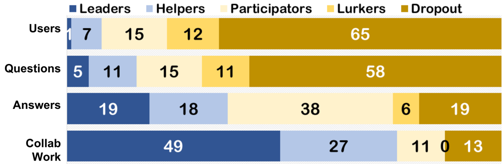
\includegraphics[width=1.0\textwidth]{figures/docent/fig-6.png}
  \caption[Distribution of role types]
{Distribution of role types for the 68 participants in the Both condition who added at least one question. The Leader formed 1\% of participants but contributed 19\% of the answers and 49\% of all collaborative activity (adding follow-ups, editing others’ question, adding options). Dropouts formed 65\% of participants and added one question each (57\% of all questions) but contributed to only 13\% of collaborative work. .\index{docent-6}}
  \label{fig:docent-6}
\end{figure}

\subsection{Emergent behavior, Engagement, and Growth}
Docent offers more avenues for active collaboration than traditional web fora. People can create questions, answer and edit questions, create follow-ups, and guess potential mechanisms. Participants added a total of 2424 answers, 74 follow-up questions, 466 new options and 358 mechanism/ discussion comments. Discussion comments fell into three types, sorted by popularity: (a) sharing personal insights; (b) sharing potential mechanisms for the question; and (c) providing links to related online resources. People edited others’ questions 119 times. Most edits were done by leaders and collaborators who attempted to clarify the question. None of the edits were reverted by the authors hinting that the edits were acceptable to them. Different ways to contribute creates different informal roles and behavior patterns in social computing systems, from leaders who perform all the activities to lurkers who may watch but not actively engage in collaborative activities (Table 4). Figure~\ref{fig:docent-6} shows the work distribution by roles in the Both condition.

Prior citizen science platforms have demonstrated lurker and dabbler behavior~\cite{Eveleigh2014}. Since people perform work on citizen science platforms, they require a prominent “circuit of engagement”~\cite{Rotman2012}. Systems research comprises many choices; some we evaluate, others follow from prior work, \& some are hunches. To counter lurker behavior, Docent employs three techniques: First, Docent encourages members’ self-selection using a strategy that hides Docent’s content (lectures, training, and the GutBoard) until people add one question. Making even small contributions makes people feel more vested in the effort as a part of a community and removes their fear of performing a novel activity~\cite{Resnick2011}. Extending these ideas can be useful for future work. Second, the GutBoard’s continuous question updates provides social translucence~\cite{Resnick2011}. Third, Docent sends regular email and social media updates to engage the community.

\subsubsection{From Asking Questions to Building a Community}
Docent’s 20 email templates cover three areas: 1) user-activity specific e.g., reminder when someone added a follow-up question to a user’s question; 2) condition-specific e.g., weekly emails about activity on the platform for the user’s condition; 3) general reminders e.g., creating a username, or adding a question if participants had not done so already. Activity emails were sent each time a user’s question received an edit, follow-up question, option, discussion comment, or when experts starred the question. Docent sent weekly general updates and links to tutorials.
 
A renowned microbiome expert recorded answers to popular questions which were subsequently mailed to participants and uploaded on social media channels. Docent maintained an active profile on Facebook and Twitter (240 and 224 followers respectively) by providing updates about platform activity, researchers’ feedback on people’s questions, and microbiome-relevant scientific articles and studies. Despite attempts to engage people, Docent saw high dropouts. Of 1630 participants, 907 (55\%) took up usernames; and 344 participants (21\%) added at least one question.

\subsubsection{Two Optimizations Significantly Improve Scaling}
To efficiently handle hundreds of participants, Docent initially renders only the first two questions while the remaining questions are rendered in the background. Docent also reduces page load times by storing markers in the browser’s local storage for frequently accessed details, e.g., last-seen question. This enables Docent to fetch and show the next question on subsequent login rather than having to pull all questions and then traverse to the last-seen question. 

\subsection{Future Work: Diversity \& Social Behavior}
Of the 344 participants who added a question, 219, who provided location information, hailed from 27 countries. 174 participants (80\%) were from US or UK who asked 76\% of questions. This is not without reason —Docent’s online publicity was focused on the American Gut Project and its offshoot the British Gut Project. However, people in these countries may have higher socio-economic, educational, and technological status than the average global (or even, national) citizen (80\% of our survey respondents had at least an undergraduate degree; an American Gut Project kit costs \$99). MOOCs face a similar challenge: educated and affluent learners complete online classes at higher rates~\cite{Kizilcec2017b}. Science and humanity will likely benefit from diverse global participants~\cite{Henrich2010a}, as in Lab in the Wild~\cite{Reinecke2015}.

Diversity brings another design challenge. Diverse participants interpret prompts like Likert scale differently. People might also use terms that are not obvious to others. For instance, one participant asked about the frequency of “hoovering your home” which likely was lost on some participants. Since Docent participants hail from dozens of countries, terms need to be understood broadly. Participants could potentially flag such questions for clarification. 

\textit{Willingness to share private information}: Only 6\% of survey respondents said they did not feel comfortable sharing personal insights. This is promising; however, there were questions that some may feel embarrassed to answer — e.g., questions pertaining to bowel movements, flatulence, and sexual activity. For these cases, questions and options can be rephrased — e.g., “Do you suffer from bouts of flatulence?” can be changed to “In the past week, how often have you suffered from flatulence?” enabling people to provide some useful information rather than entirely avoiding such questions. Moreover, specific communities’ motivation can be focused on generating specific insights~\cite{Chandler2013}. Docent already has many questions raised by participants suffering from different ailments; such patient groups may have specific insights as well as greater motivation to share them in exploratory projects~\cite{Karkar2017a}.

\textit{Different strokes for different folks}: Docent users were volunteers. Multiple survey respondents mentioned that busyness impeded their platform usage. We hypothesize that encouraging moderators may increase platform stickiness. We plan to create guides and have people try different roles which can boost creative thinking~\cite{Teevan:2017:BWC:3059454.3059467}. With a diverse participant set — health-hackers, MOOC learners, even some advanced microbiome students — people’s attention can be put to specific tasks that they want to contribute to. For instance, MOOC learners may be more interested in unearthing mechanisms for people’s hypotheses. Such differentiated roles, including different levels of editor, have contributed to the success of social computing systems like Wikipedia~\cite{Krieger2009}.

\textit{Validating hypotheses shared by participants}: One early benefit of our work is that American Gut researchers are using the best Docent questions to potentially add/revise the metadata catalogue in the American Gut Project. Moreover, with the right online support, citizens can design and run experiments to test some of the hypotheses (e.g. probiotics reduces sugar cravings). Scaling causal reasoning could transform many domains. One interested party is the non-profit Open Humans platform where people volunteer their personal data (e.g., microbiome/genomic data) and provide access to researchers to use their data.

%%%%%%%%%%%%%%%%
\section{Conclusion}
This paper investigated integrating learning and training with online scientific work. Experts rated 75 of 399 questions as potentially scientifically novel. Participants with access to process training generated hypotheses of better quality. Access to learning materials improved the questions’ microbiome-specific knowledge.  The Learn-Train-Ask method can be applied towards next steps in the scientific process, namely designing and running experiments. This study also illustrates the challenges of designing a social computing system that engages voluntary participants in performing personally-relevant scientific work. Such online experiences also naturally provide a problem-based learning setup for better learner engagement. Intui-tions gathered from a large online crowd can significantly scale up scientific inquiry by augmenting scientific expertise with insights and know-how drawn from the lived experiences of diverse individual people. We believe that dual-objective online systems that combine learning with personally meaningful work can enable people to meet their needs.



\chapter{Collaboratively Running Experiments}
\begin{quote}
\emph{People have creative scientific questions and folk theories;
yet most lack the expertise to investigate them. How might
people transform their questions into experiments that
inform both science and their lives? This chapter introduces
the Galileo system}; it provides procedural support using
three techniques: 1) experimental design workflow that
provides just-in-time training; 2) review workflow with
scaffolded questions; and 3) automated routines for data
collection. We present three empirical investigations: a
between-subjects experiment with students, a study with
online volunteers across 16 countries, and a deployment
with online volunteers across 8 countries. Procedural
support yielded higher-quality experiments than watching
lecture videos. People generated structurally-sound experiments
on personally meaningful topics and ran them with
participants from around the world.
\end{quote}

\begin{figure}[h] 
  \centering
  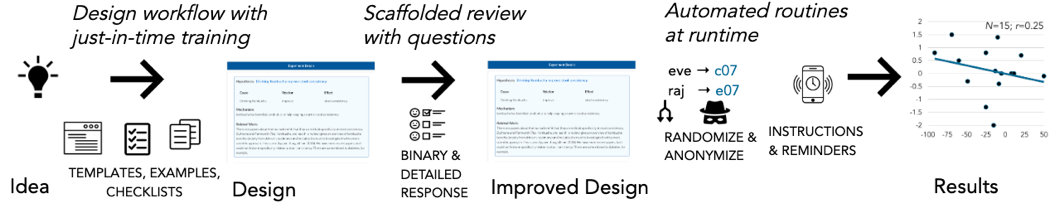
\includegraphics[width=0.9\textwidth]{figures/galileo/galileo-1}
  \caption[Galileo enables anyone to design and run experiments to test their intuitions]
{Galileo enables anyone to design and run experiments to test their intuitions. Experiment creators can invite anyone to review and participate in the experiment. Participants from around the world join experiments, follow instructions, and provide data in response to automated data collection reminders.\index{galileo-1}}
  \label{fig:galileo-1}
\end{figure}

\vspace{0.25in}

%%%%%%%%%%%%%%%%%%%%%%%%%%%%%%%%%%%%%%%%%%%%%%%%%%%%%%%%%
\section{Experience to Experiments: Self-tracking Offers Insights but Not Causality}
People have questions about their health, but lack the expertise and resources to scientifically
investigate them. These concerns are especially acute when multiple factors interact. Despite
knowledge gained from lived experiences, people lack the procedural tools to gain the causal
knowledge they seek. Many self-tracking efforts suffer from structural flaws that prohibit people
from actually learning what they'd like to know~\cite{Choe2014, Li2010a}. A frequent error is mistaking correlation
for causation~\cite{Munroe2009}. People falsely believe that when one event follows another, the initial event is
the cause: post-hoc ergo propter hoc. At the same time, professional science suffers from structural
biases. By creating controlled experiments (as opposed to tracking oneself), people can test their
intuitions at a larger scale, potentially unearthing novel results. How can we train people in designing
and running experiments to answer their personally-meaningful questions?

Scientific experimentation features technical requirements and contextual choices that are inscrutable for a lay individual yet necessary for success~\cite{Martin2007}. While professional scientists and commercial ventures run experiments every day, with notable exceptions~\cite{Cooper2010, Lewis2016}, empirical papers from non-professionals are vanishingly rare. This biases the questions asked, studies run, and knowledge created~\cite{crawford2017politics,Henrich2010a}. People have questions about their health, but lack the expertise and resources to scientifically investigate them. Broadening the pool of experimenters could help people investigate their curiosities, develop solutions to improve health and performance, and assist institutional researchers.

The main contribution of this chapter is \textit {demonstrating that online volunteers can collaboratively perform scientific experimentation}. It does so in two main ways: 1) procedural support for acquiring domain expertise using three techniques: experimental design workflow that provides just-in-time training, review with scaffolded questions, and automated routines for data collection; and 2) the Galileo social computing system that instantiates procedural support for citizen experimentation (Figure~\ref{fig:galileo-1}). 

Three empirical investigations tested Galileo's approach. First, a controlled between-subjects experiment with 72 participants found that procedural support yielded significantly higher-quality experiment designs than lecture videos. Second, a deployment across 16 countries found that people generated structurally-sound experiments on personally meaningful topics. Third, in a field deployment, online users from three communities---kombucha, Open Humans, and beer---across 8 countries demonstrated that people designed, iterated on, and ran week-long experiments.

%%%%%%%%%%%%%%%%%%%%%%%%%%%%%%%%%%%%%%%%%%%%%%%%%%%%%%%%%
\section{The Galileo Experimentation Platform}
Galileo introduces a system for end users to design experiments, get them reviewed, and run them with interested participants. It provides procedural support for these steps, an online collaboration platform, and automated data collection and reminders.

Despite a predetermined goal and a formalized process, experimentation requires making contextually-appropriate decisions~\cite{Martin2007}. Good experiment design is inherently user centered; designers need awareness of others' interpretation of their ideas and asks. Providing feedback on experiment designs requires knowing the success criteria and how to help improve.

%\begin{wrapfigure}[23]{r}{0.5\textwidth}
%%\vspace{-0.25pt}
%  \centering
%  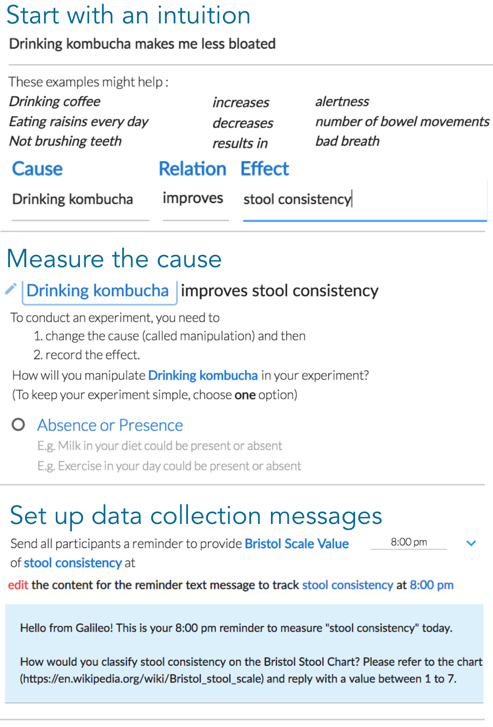
\includegraphics[width=0.48\textwidth]{figures/galileo/galileo-2-design}
%  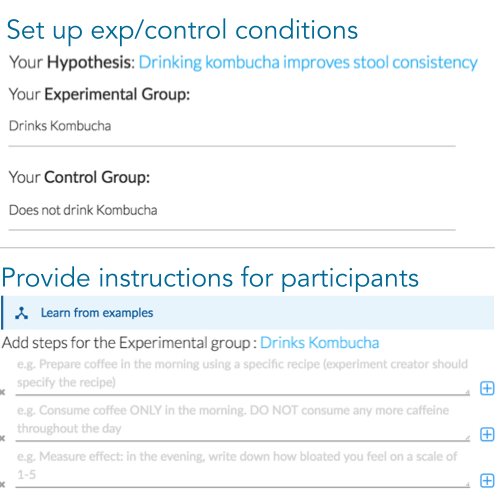
\includegraphics[width=0.48\textwidth]{figures/galileo/galileo-2-design-2}
%  \caption[Galileo's design module helps people transform intuitions into experiment designs]
%{Galileo's  design module helps people transform intuitions into experiment designs. It walks people through 1) converting an intuition to a hypothesis, 2,3) providing ways to manipulate/measure cause and effect, 4-5) specifying control and experimental conditions, and (not shown) providing inclusion/exclusion criteria.\index{galileo-2}}
%  \label{fig:galileo-2}
%\end{wrapfigure}

\begin{figure}[h]
%\vspace{-0.25pt}
  \centering
  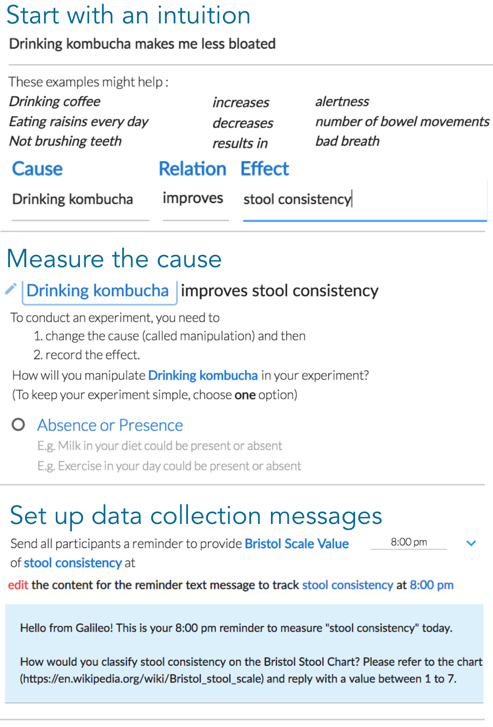
\includegraphics[width=1.0\textwidth]{figures/galileo/galileo-2-design}
%  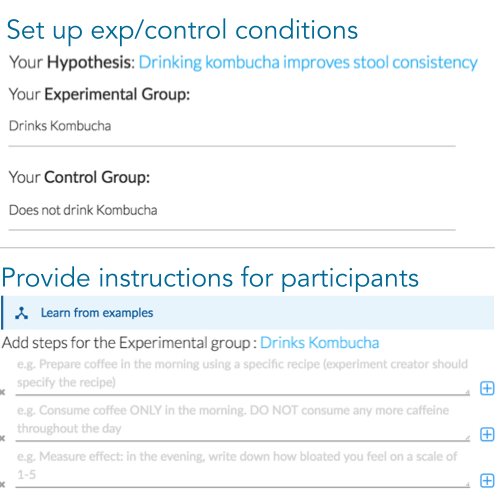
\includegraphics[width=0.48\textwidth]{figures/galileo/galileo-2-design-2}
  \caption[Galileo's design module helps people transform intuitions into experiment designs]
{Galileo's  design module helps people transform intuitions into experiment designs. It walks people through 1) converting an intuition to a hypothesis, 2,3) providing ways to manipulate/measure cause and effect, 4-5) specifying control and experimental conditions, and (not shown) providing inclusion/exclusion criteria.\index{galileo-2}}
  \label{fig:galileo-2}
\end{figure}

Finally, successfully running an experiment requires managing multiple processes such as random assignment, anonymizing participant details, and sending instructions and reminders for data collection.

\subsection{Design-Review-Run: From intuitions to investigations}
Galileo requires three roles for each experiment: designer, reviewer, and participant. Galileo offers procedural support for each: 1) a design workflow provides just-in-time training, 2) review with scaffolded questions, and 3) automated routines for runtime activities like data collection. Users form and refine with the help of contextual support and learning resources from the system. 

\subsection{Design an experiment from an intuition}
People have many, often poorly-framed, hypotheses. Galileo's design workflow helps people harvest and sharpen them (Figure~\ref{fig:galileo-2}). Examples illustrate possible choices and how they relate; templates provide structure; and embedded videos explicate technical issues. Such procedural support can improve on-task performance~\cite{Pandey2018}. A final self-review step provides an overview of the experiment. To keep the platform safe, the primary author receives daily updates of platform activity. The design workflow does not mandate double-blindness or the use of placebo; designers can choose to specify these details.

%\begin{wrapfigure}[10]{r}{0.5\textwidth}
%  \centering
%  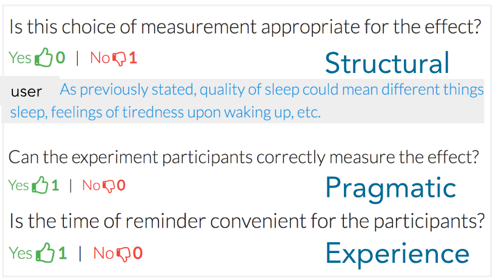
\includegraphics[width=0.5\textwidth]{figures/galileo/galileo-2-review}
%  \caption[Reviewers walk through an experiment providing binary rubric assessments]
%{Reviewers walk through an experiment providing binary rubric assessments. A No response prompts reviewers to provide concerns and suggestions.\index{galileo-2-review}}
%  \label{fig:galileo-2-review}
%\end{wrapfigure}

\begin{figure}[h]
  \centering
  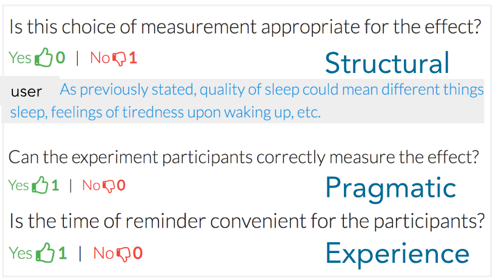
\includegraphics[width=0.5\textwidth]{figures/galileo/galileo-2-review}
  \caption[Reviewers walk through an experiment providing binary rubric assessments]
{Reviewers walk through an experiment providing binary rubric assessments. A No response prompts reviewers to provide concerns and suggestions.\index{galileo-2-review}}
  \label{fig:galileo-2-review}
\end{figure}

\subsection{Review the design via feedback from others}
Galileo experiments require at least two reviews before they can be run. The designer invites the reviewers, who might be online community members, a teacher, or anyone else who can provide useful feedback. Upon receiving reviews, the designer edits the experiment to address any issues. For research purposes, Galileo logs version changes. Reviewers provide both binary assessment and written responses to specific questions (Figure~\ref{fig:galileo-2-review}). These questions cover structure (e.g., accounting for confounds), pragmatics (e.g., measuring the real-world cause/effect), and participant experience (e.g., data reminder time). Reviewers are ineligible to be participants in the same experiment. Similarly, creators may not review their own experiment. 

%\begin{wrapfigure}[17]{r}{0.5\textwidth}
%  \centering
%  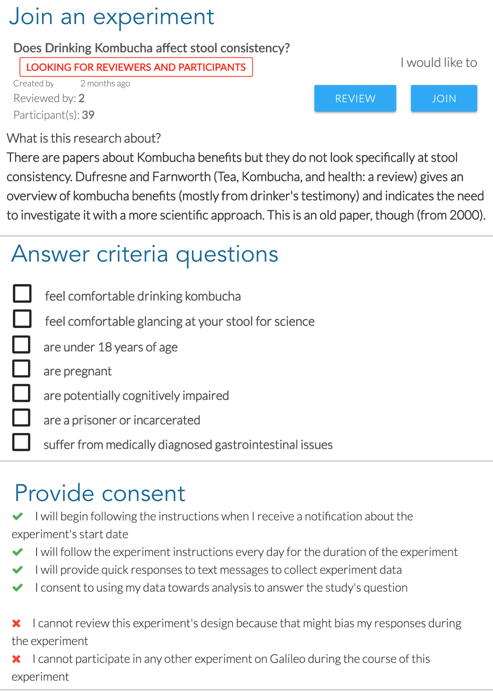
\includegraphics[width=0.5\textwidth]{figures/galileo/galileo-2-run}
%  \caption[Join workflow for participants]
%{Join workflow for participants. 1) Participants can view a list of experiments. When they elect to join one, they 2) answer inclusion/exclusion criteria, 3) consent to following the provided steps, and 4) receive instructions. Participants receive daily, condition-specific requests, and respond with data and/or clarifying questions. \index{galileo-2-run}}
%  \label{fig:galileo-2-run}
%%\vspace{-1pt}
%\end{wrapfigure}

\begin{figure}[!h]
  \centering
  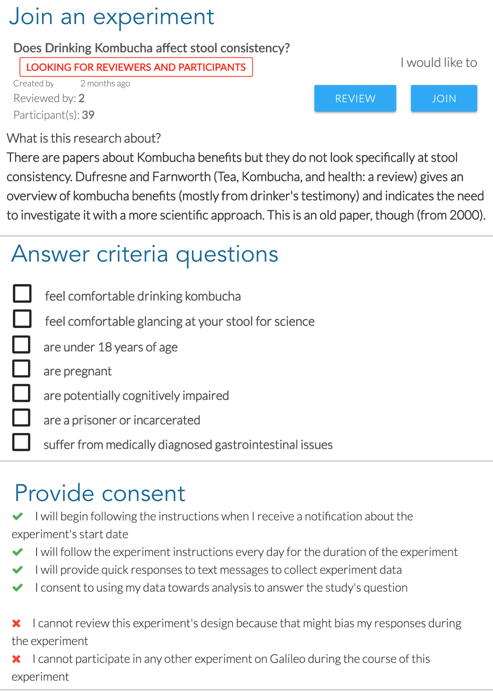
\includegraphics[width=0.5\textwidth]{figures/galileo/galileo-2-run}
  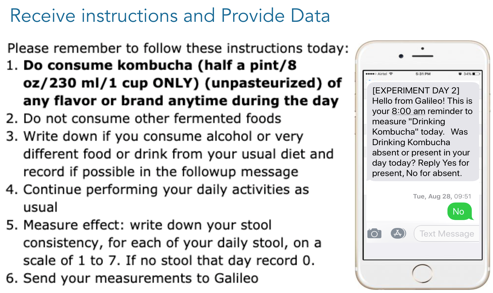
\includegraphics[width=0.5\textwidth]{figures/galileo/galileo-2-run-01}
  \caption[Join workflow for participants]
{Join workflow for participants. 1) Participants can view a list of experiments. When they elect to join one, they 2) answer inclusion/exclusion criteria, 3) consent to following the provided steps, and 4) receive instructions. Participants receive daily, condition-specific requests, and respond with data and/or clarifying questions. \index{galileo-2-run}}
  \label{fig:galileo-2-run}
%\vspace{-1pt}
\end{figure}

\subsection{Run an experiment using procedural support}
To launch an experiment, its designer shares a unique URL with potential participants. Galileo automatically manages four activities to reduce bias and workload:
\begin{enumerate}
\item Randomized placement of people into conditions~\cite{Martin2007}.
\item Maintain a per-experiment participant map ([usernames]$\rightarrow$ [exp$\textunderscore$id]) for anonymity
\item Collect and clean data (sending data collection messages and reminders at time zone appropriate times, parsing the responses, updating participant and experimenter views). 
\item Prompt experimenters to perform tasks when conditions are met (e.g., setting the start date when enough participants have joined or reminding participants with missing data). 
\end{enumerate}

Participation comprises following instructions (e.g., drink kombucha) and providing self-report responses to platform queries (Figure~\ref{fig:galileo-2-run}). The current implementation supports email, SMS, and WhatsApp. Self-reports provide the primary data collection mechanism. Participants can optionally answer follow-up questions that capture contextual insights. Galileo logs responses to a MongoDB database. Galileo presents participant data to experimenters using participant ID rather than real name or username. When the experiment ends, participants receive a summary of results. Participants can anonymously discuss the experiment at the end, so the experimenter can learn from their feedback. 

The experimenter's dashboard lists tasks: answer clarifying questions, remind/thank participants, or look at trends in data (Figure~\ref{fig:galileo-2-run-1}). Experiments have a minimum participation count; there's no upper limit to the number of participants. People who sign up after a cohort begins are added to a waitlist.
The Galileo web application uses the Meteor (meteor.com) framework for synchronization, Jade for the front end (jade-lang.com), Materialize for styling (materializecss.com), and Twilio as the text message gateway (twilio.com).

\begin{figure}[!h] 
  \centering
  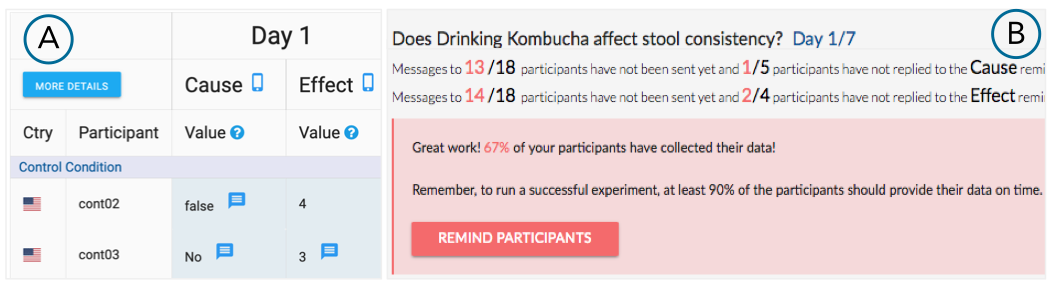
\includegraphics[width=1.0\textwidth]{figures/galileo/galileo-2-run-1}
  \caption[Galileo takes care of many experimenter responsibilities such as random placement of people, sending instructions and reminders, and cleaning and displaying data in both participant and experimenter dashboard]
{Galileo takes care of many experimenter responsibilities such as random placement of people, sending instructions and reminders, and cleaning and displaying data in both participant and experimenter dashboard. The dashboard enables experimenters to A) remind those with missing data; and B) see participants' data; and clarify questions raised by participants.\index{galileo-2-run-1}}
  \label{fig:galileo-2-run-1}
\end{figure}

\subsection{Designing the platform}
More than 80 people have designed and run experiments. The system design evolved over a year of weekly in-person user-centered studies with lead users from different communities including kombucha and self-tracking enthusiasts. The pilot study gathered feedback on the usefulness of the interface items and resources. Students in an undergraduate Psychology class (Introduction to Research Methods) also used Galileo in a 90-minute classroom deployment to rapidly design and review each others'experiments and receive feedback. We provide three examples of how pilot studies informed Galileo's design:

\begin{enumerate}
\item \textit{Embedded written training over videos}: Early versions provided short, online lecture videos as the learning materials. Most users did not watch them end-to-end to extract the step-relevant insight(s). In response, each step's content now offers written examples, which are easier to skim and refer back to. 

\item \textit{Supporting actionable feedback}: For the review interface, early versions only requested binary Yes/No responses similar to popular crowdsourcing platforms; both experiment designer and reviewers found this to be unsatisfactory. Galileo now provides a prompt for actionable feedback whenever the reviewer selects "No" to any question. 

\item \textit{Ease of glancing at participants' data}: Pilot users ran six trial experiments. The idea of a runtime dashboard (Figure~\ref{fig:galileo-2-run-1}A) came from observing experimenter's difficulty tracking participants' data and sending reminders to those who hadn't added their data. Participants struggled with making suitable preparations for a week of experimentation (e.g. buying sufficient kombucha). The system now prompts experimenters to explicitly add preparation instructions that are sent to participants 2 days before the experiment begins. 
\end{enumerate}

\subsection{Integrating procedural support in the design workflow}
Simple examples of procedural learning are activities like tying your shoes, roasting a chicken, or replacing a door handle. Recipes and instructions convey procedures in written form; demonstrations and hands-on learning make it more interactive. Creative tasks differ from rote procedures in that they require people to generate some artifact themselves.

\subsubsection{Embedding Just-in-Time Support}
Complex activities overwhelm learners' working memory because of their many interrelated pieces~\cite{Engle2002}. Recalling work from previous steps and frequent context-switching are especially taxing~\cite{Gonzalez2004}. Experts mitigate memory demands by integrating multiple elements into conceptual chunks~\cite{Chase1973}. A well-chunked interface can still require knowledge that novices lack. Galileo provides missing knowledge by providing learning materials in the interface. This \textit{in-situ} embedding has three advantages: it is minimal~\cite{Carroll1987}, leverages teachable moments~\cite{Havighurst1953}, and can be ability-specific~\cite{Corbett1997}. Finally, as is good user interface practice, selecting good defaults for each step helps users see an example of appropriate choices. 

Early Galileo users sometimes made poor choices, like listing effects that are difficult to measure. To help guide people, Galileo now presents a short checklist for verifying the choices made in each section. This self-review provides lightweight, just-in-time support.

\subsubsection{Example: Training people to identify a cause}
Controlled experiments seek to identify develop causal understanding by varying just the cause in experimental conditions. Many people do not understand the importance of having this minimal-pairs design, perhaps because they do not have the same issues in mind when thinking about the cause as when thinking about the conditions.

Galileo administers the following process to help designers select conditions that test a causal claim. It provides a simple description in common English with ~3 examples showing the data collection reminder text and times right after the designer decides on the cause and effect metrics. Galileo auto-populates text reminders with readable sentences~\cite{Levy2013} that people can edit. Finally, checklists help people review and improve their work. Such checklists refer to more context-specific challenges of making the experiment simple, safe, and comfortable for participants.
 
Three studies evaluated Galileo's approach: a controlled experiment to test procedural support's efficacy in the design workflow; a field study to test whether people can create structurally-sound experiments based on personal intuitions; and a deployment to test whether people can design and run experiments. 

%%%%%%%%%%%%%%%%%%%%%%%%%%%%%%%%%%%%%%%%%%%%%%%%%%%%%%%%%
\section{Study 1: Experiment Comparing Procedural Support to Videos}
To investigate whether procedural support helps novices design experiments, a between-subjects experiment tested the following hypothesis: \textbf{\textit{Procedural support yields higher quality experiment designs than lecture videos}}. 

Procedural training, when successful, helps people solve unique problems with similar structure. It is perhaps best studied in K-12 mathematics instruction~\cite{Rittle-Johnson1999}. We hypothesize that participants who use interactive procedural support create better experiment designs than those who watch videos on the topic. 

\subsection*{Method}
Participants were randomly assigned to one of two conditions: \textit{Videos} or \textit{Galileo} (Figure~\ref{fig:galileo-6-study}). The \textit{Videos} condition provided a playlist of videos about experiment design from a Coursera MOOC that operationalized the task-specific concepts~\cite{Wobbrock2018}. The \textit{Galileo} condition provided participants access to Galileo. Both provided the same content for creating a structurally-sound experiment. Moreover, participants were provided instructions that the resources (videos/Galileo) described the attributes that their designs should possess. Scripted study instructions ensured the same manipulation. 

The study asked participants to compose an experimental design for a personal intuition of their choosing. Each condition provided informational resources and a means to document their design (videos with a text document, or procedural support with inline text fields). Participants were told that there was no lower or upper time limit. Each session comprised the following steps: consent, design task, survey, and interview. Participants could also use web resources--- such as Wikipedia---and many did. The interview asked participants about confidence in their experiment design abilities and their experience using the system. The interview was tailored to participants' behavior and survey responses: for example, if a participant did not watch some videos, the interviewer asked why. An independent rater (a professor who teaches experiment design) blind to condition rated each participant's experiment using the rubric (Table~\ref{tab:rubric1}).

\begin{figure}[t] 
  \centering
  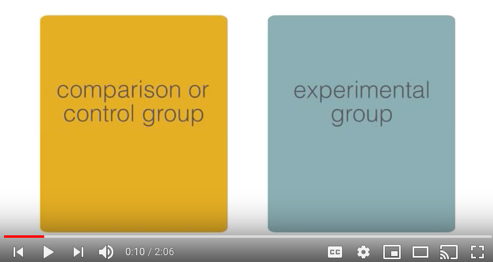
\includegraphics[width=0.48\textwidth]{figures/galileo/galileo-study-1}
  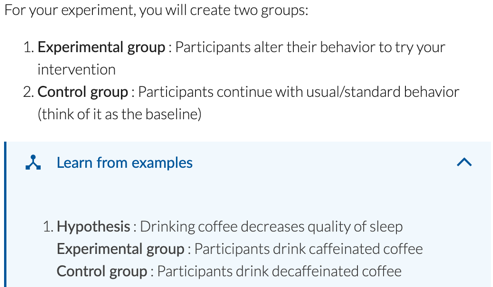
\includegraphics[width=0.48\textwidth]{figures/galileo/galileo-study-2}
  \caption[Two conditions for experiment: \textit{Videos} and \textit{Galileo}]
{Two conditions for experiment. In the \textit{Videos} condition, participants accessed videos about experiment design. In the \textit{Galileo} condition, participants accessed Galileo tool (which included the videos if participants wanted to see them). Both conditions provided the same content. \index{galileo-6-study}}
  \label{fig:galileo-6-study}
\end{figure}

%%%% TABLE 1 %%%%
\vspace{0.25in}
\begin{table}[!ht]
\caption[Demography information for 72 participants (all undergraduate students)] 
{Demography  information for 72 participants (all undergraduate students). Some participants did not complete portions of the survey.}

\vspace{-0.25in}
\begin{center}
\renewcommand{\arraystretch}{1.5}
%\begin{tabular}{c >{\em}c c}
\begin{tabular}{>{\bf}p{1.5in}p{1.75in}p{1.75in}}
\hline
Nationality	&	USA=37		&	China=11\\
			&	No Answer = 6	&	Others = 18\\
Gender		&	Female = 47	&	Male = 24\\
Native English	&	Yes = 38 		&	No = 34\\
Age			&	18-20 = 40	& 	26-30 = 1\\
			&	21-25= 31	&			\\
Ethnicity		&	Asian/Pacific=36 & 	Hispanic/Latino=14\\
			&	White = 11		&	Others=11 \\
Major		&	Biology=12	& 	Psychology=20 \\
			&	Cognitive Sci=12 &	 Others = 20 \\
Used online	& 	Never=28		&	Occasional=16\\
learning		&	1 class=11	&	2-5 classes=12\\
\hline
\end{tabular}
\end{center}
\label{tab:gi-results1}
\end{table}


\subsection*{Participants}
\textit{Recruitment}: 72 participants were recruited from a Western US Research University (Table~\ref{tab:gi-results1}). 11 had no prior experience with experiment design; 61 had taken a course or equivalent. Expertise was counterbalanced across conditions.

\subsection*{Measures}
The independent variable is access to Galileo/videos. The study scored experiments via a 13-question rubric (Table~\ref{tab:rubric1}), and recorded time taken. A blind-to-condition expert (a regular instructor of large, undergraduate courses on experiment design) provided the scores. Qualitative measures included how participants used the tool, where they faced challenges, and a post-experiment survey. A non-parametric Mann-Whitney test assessed the effect of condition on design quality.

%%%% TABLE 2 %%%%
\vspace{0.25in}
\begin{table}[!ht]
\caption[Rubric for design-quality criteria for structure]
{Rubric for design-quality criteria for structure}

\vspace{-0.25in}
\begin{center}
\renewcommand{\arraystretch}{1.5}
\begin{tabular}{p{1.75in}p{3.5in}}
\hline
\textbf{\textit{Hypothesis}: 3 points} & Is the cause/relation/effect specific?  \\
\textbf{\textit{Measurement}: 2 points} & Are the cause and effect manipulated/measured correctly? \\
\textbf{\textit{Conditions}: 3 points}  & Are the control and experimental conditions appropriate? 2 points \\
 & Do the conditions differ in manipulating the cause? 1 point \\
\textbf{\textit{Steps}: 2 points}  & Are experimental steps clear for control/experimental conditions?  \\
\textbf{\textit{Criteria}: 2 points} & Are the exclusion criteria correct and complete? Are the inclusion criteria correct? \\
\textbf{\textit{Overall}: 1 point} & Can the overall experiment be run as is?  \\
\hline
\end{tabular}
\end{center}
\label{tab:rubric1}
\end{table}

%\subsection*{Results}
\subsection{Access to Galileo improved the quality of experiment design}

%\begin{wrapfigure}{r}{0.5\textwidth}
%  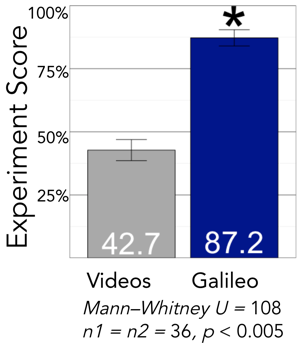
\includegraphics[width=0.5\textwidth]{figures/galileo/galileo-study1-7}
%  \caption[Access to Galileo improved the quality of experiment design]
%{Access to Galileo improved the quality of experiment design\index{galileo-study-1}}
%  \label{fig:galileo-result}
%\end{wrapfigure}

\begin{figure}[h]
\centering
  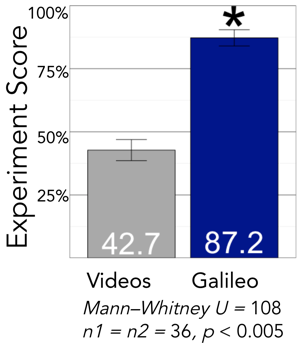
\includegraphics[width=0.5\textwidth]{figures/galileo/galileo-study1-7}
  \caption[Access to Galileo improved the quality of experiment design]
{Access to Galileo improved the quality of experiment design\index{galileo-7-result}}
  \label{fig:galileo-7-result}
\end{figure}

\textit{Galileo} participants created higher-quality experiments (M = 11.3) than \textit{Videos} participants (M = 5.6); Mann–Whitney U = 108, n1 = n2 = 36, p $<$ 0.005 (Figure~\ref{fig:galileo-7-result}). Of the 36 designs rated in the top half, 29 were from \textit{Galileo} condition. \textit{Galileo} participants performed better on five out of six sections (all except hypothesis). There was no significant difference in the amount of time participants spent creating an experiment in the \textit{Videos} condition (M = 30.8 mins) vs \textit{Galileo} (M = 29.0 mins) conditions; Mann–Whitney U = 734, n1 = n2 = 36, p = 0.33 two-sided. 

\subsection*{Discussion}
As Galileo aims to improve tasks like experimental design, Study 1's primary dependent variable was quality (as opposed to learning gains). Online video resources represent a common status quo: contemporary and bite-sized yet still static resources. This comparison enabled us to observe how Galileo's procedural support changed design outcomes. \textit{Videos} participants followed one of two strategies: 1) watch all the videos at once and then begin writing the experiment; or 2) begin designing the experiment and use the videos to fill in the gap when stuck. Like cramming, all-at-once watching floods the mind, perhaps making it difficult to use seen ideas~\cite{kornell2009optimising}. By contrast, the search-when-needed approach interrupts people's flow, replacing the attention on design with a task of locating needed information. \textit{Videos}' lower score and our observations, in conjunction with the literature, suggest contextually-integrated approaches like procedural support increase people's useful adoption of information.
   
Participants reported that the videos were slow and the interface provided sufficient examples. Participants in the \textit{Galileo} condition opened and closed the videos in quick succession. Participants in the \textit{Videos} condition, however, felt that the videos provided a refresher of some concepts they vaguely knew about. Did too much information (e.g. the inclusion of other concepts) in the Coursera course dilute performance? It's possible; accessing the "right" moment in videos is a known research question~\cite{kim2014crowdsourcing}. 

Participants in both conditions expressed a lack of confidence in their chosen cause/effect measures. Some spent over 15 minutes searching for measures: one found a formal sleep-quality scale from Stanford researchers. Participants in both conditions mentioned that they enjoyed reflecting on their lifestyle/health ideas and thinking through how to transform an intuition into an experiment. Participants wished that Galileo was integrated with their class, describing it as "hands on" and "DIY". 

\subsection*{Limitations}
This experiment found procedural support to yield higher-rated designs than watching videos. Important direction for future work will be to compare different approaches to procedural support, and exploring additional measures (e.g., novelty). 

%%%%%%%%%%%%%%%%%%%%%%%%%%%%%%%%%%%%%%%%%%%%%%%%%%%%%%%%%
\section{Study 2: People Design \& Review Experiments Online}
The first study evaluated the efficacy of procedural support for designing experiments. The second study investigated the quality and nature of experiments; specifically, whether people a) create experiment designs that are structurally-sound, demonstrate insights from lived experiences, and have novel ideas, and b) provide useful feedback on experiment designs. 

\subsection*{Method}
Participants used Galileo to design their experiments and review others'. Galileo's landing page described why experiments are important and the importance of citizens' contributions towards making discoveries. Upon logging in, participants could design an experiment (see Figure~\ref{fig:galileo-2}), review existing experiments (see Figure~\ref{fig:galileo-2-review}), or join an experiment (see Figure~\ref{fig:galileo-2-run}). 

\subsection*{Recruitment}
Participants were recruited via online publicity. One recruitment focus was people curious about the microbiome because it is a domain where lived experience may inspire intuitions, and the science is nascent~\cite{McDonald2018a}. Galileo was promoted on the American Gut's and their collaborators' Facebook and Twitter pages. Galileo was added as a project on Open Humans (openhumans.org), posted on multiple subreddits pertaining to health and lifestyle, and introduced as an optional activity in assignments on the Gut Check Coursera MOOC~\cite{Knight2016}. Participation was voluntary and unpaid. 


%%%% TABLE 3 %%%%
\vspace{0.25in}
\begin{table}[!ht]
\caption[Rubric for design-quality criteria for Structure, Content, and Novelty]
{Rubric for design-quality criteria for Structure, Content, and Novelty}


\vspace{-0.25in}
\begin{center}
\renewcommand{\arraystretch}{1.5}
\begin{tabular}{p{1.5in}p{4in}}
\hline
\textbf{Structure} &  \textit{Described in Table~\ref{tab:rubric1}} \\
\textbf{Content}  & \\
~~\textit{Personal?} & Did the hypothesis draw from lived experience? \\
~~\textit{Popular?} & Is the world already curious about this hypothesis (e.g. discussions on online fora)?  \\
~~\textit{Insightful?} & Does the hypothesis link to existing science?  \\
\textbf{Novelty}  &  Is there a chance the world will learn something: absence of published research for this question?\\
\hline
\end{tabular}
\end{center}
\label{tab:rubric2}
\end{table}

\subsection*{Measures}
Measures comprised structure, content, and novelty of experiment designs (Table~\ref{tab:rubric2}) and usefulness of reviews. Raters with training in experiment design independently rated participants' work, then discussed them to form a shared view of assessment. Next, each independently rated all experiments. The final score is the mean of their independent ratings. Moderate reliability was found between the two raters' measurements~\cite{koo2016guideline}; m(ICC) = .62, 95\% CI [.45, .75], (F(64,64)= 4.33, p$<$.001. 

Structure measures whether the design is correct and includes appropriate components. Content measures the subject matter of the idea driving the experiment design; it was rated as personal focus, popularity, and insightfulness of the hypothesis. Novelty was assessed as the potential to create new knowledge and operationalized as the lack of research papers about the specific hypothesis. Raters were instructed to assign points for a component (say hypothesis) if the experiment provided appropriate details about it. For example, the hypothesis \textit{Text message reminder increases consumption of recovery snack} was rated to have a specific cause, a specific effect, and a clear relation between the two, while \textit{Eating too much energy causes disturb [sic] sleep cycle} did not have a clear cause or effect. \textit{Ingesting non-local food results in poor evacuation of fecal matter} '' was rated as novel because no published research addresses this (as per Google Scholar). Broad or vague hypotheses related to well-studied topics were not deemed novel (e.g. \textit{Going to college increases grades}).

54 users from 16 countries created 66 complete experiment designs (Mdn=27 minutes). 37 users provided 205 descriptive review comments. Latest versions of complete experiment designs were scored as described above; incomplete experiments and older versions were removed from analysis. 

\subsection*{Results}
%\subsubsection{People Designed Structurally-Sound Experiments, and Drew from Personal Intuitions}
\subsection{People design structurally-sound experiments, and draw from personal intuitions}
The mean score for the experiment was 10.3/13. On average, people scored higher than 75\% on 8 of 13 measures. 38\% of experiment designs came for people's lived experiences; e.g., \textit{eating yogurt makes a person have a more regular bowel movement}. Personal health and performance were big draws: 90\% of experiments sought to improve a health outcome. 

\begin{figure}[h]
\centering
  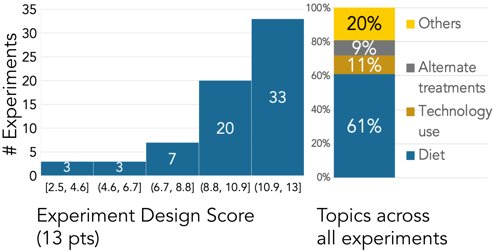
\includegraphics[width=0.7\textwidth]{figures/galileo/galileo-study2-1}
  \caption[Results: Most experiments were structurally-sound and drew from personal experiences]
{A) Most experiments were structurally-sound, scoring high on the structure rubric. B) Most experiments drew from personal experiences \index{galileo-8-result}}
  \label{fig:galileo-8-result}
\end{figure}

51\% of the experiments were rated as popular; their hypotheses were discussed on other online fora; e.g., \textit{having dry mouth (or Sjogren's Syndrome) promotes the growth of less beneficial gut microbes}. Common themes included diet (dietary styles, alcohol, fermented foods), technology use (social media, laptop, mood) and alternative treatments (homeopathy), and health (sleep, pain, gut issues) (Figure~\ref{fig:galileo-8-result}). Apart from being structurally-sound, the best experiment designs shared two features: they shared a personal experience and linked to known research. For example, a user designed an experiment to test yogurt's effect on bowel movement and shared their motivation: 

\textit{\say{For several months I have been producing Yogurt. This is fermented using commercial probiotics, Probiotic-10. My intuition was that since various microbe species were active in the making of the yogurt, this product can help relieve of the various digestive problems one persona can have. It happens that one of my sons was diagnosed with Ulcerative Colitis. among other things he was losing weight rapidly. After several weeks of consuming probiotics and/or the yogurt, he begun to recover.}}

17\% of hypotheses had novel insights that no published research addresses. For instance, \textit{Avoiding foods high in lectins cures long-term post-infectious diarrhea} and \textit{Drinking kombucha regularly reduces joint inflammation/arthritis symptoms} are both hypotheses of interest to citizens and microbiome researchers alike.

%\begin{wrapfigure}[8]{r}{0.5\textwidth}
%\centering
%  \includegraphics[width=0.48\textwidth]{figures/galileo/galileo-study2-1}
%  \caption[Results: Most experiments were structurally-sound and drew from personal experiences]
%{A) Most experiments were structurally-sound, scoring high on the structure rubric. B) Most experiments drew from personal experiences \index{galileo-study2-1}}
%  \label{fig:galileo-result2}
%\end{wrapfigure}

\begin{figure}[h] 
  \centering
  \includegraphics[width=0.66\textwidth]{figures/galileo/galileo-study2-2}
  \includegraphics[width=0.33\textwidth]{figures/galileo/galileo-study2-3}
  \caption[Result: Review comments were distributed across all components of experimental design]
{Summary of review A) Review comments were broadly distributed across all components of experimental design. B) Review comments ranged from 3 chars "yes" to 871 char long descriptions. C) The longest review comment described multiple problems with an experimental design while providing numerous actionable suggestions. \index{fig:galileo-9-result}}
  \label{fig:galileo-9-result}
\end{figure}

%\subsubsection{Reviewers Use Domain Knowledge to Improve Designs and Advocate for Participant Experience}
\subsection{Reviewers use domain knowledge to improve designs and advocate for participant experience}
158 review comments (77\%) were rated useful; incorporating them would improve the experiment. Average comment length was 140 characters ranging from 3 characters (\textit{yes}) to 871 characters (Figure~\ref{fig:galileo-9-result}B,C). Most comments were direct responses to a rubric question hinting that the review interface helped people focus on the salient parts of an experiment design.

The most common comments sought improving structural correctness (38\%) by requesting specific details. For example, one reviewer questioned an experiment's choice of Likert scale for mood saying, \textit{A simplistic Likert scale seems like a bad idea. There has to be something better than this. At least a couple questions? Like, optimism, excitement, depression, anxiety?}. Reviewers provided the most comments (54\%) about the hypothesis and cause \& effect measures. People advocated for improving participant's experience (18\%). Suggesting better data collection messages and times was a popular theme. We present two examples: 1) \textit{People are not very good at remembering what they eat. Maybe an App like MyFitnessPal would be useful since it would allow participants to track all the food they eat without having to remember for too long}, and 2) \textit{How long do they [experiment participants] have to answer? What if they're eating dinner and can't get to it until 9pm?}.

14\% of comments demonstrated domain-specific knowledge E.g., one reviewer pointed out a conceptual mistake about a Type-1 diabetes experiment: \textit{A1C is measured monthly and won't change after 1g. You mean the BG value?} A1C refers to the average blood glucose value average levels over the past 3 months that is less susceptible to short term changes. BG here refers to the blood glucose value that depends on immediate glucose intake (among other factors). Surprisingly, reviewers barely drew from their personal experience when suggesting improvements (or at least, did not explicitly mention this was their personal experience). Some comments drew on counterfactual reasoning while thinking about how participants might "hack" an experiment. A comment on an experiment about social media use and steps walked asked, \textit{…the timing of this [reporting steps taken] vs. social media use measure is off and that makes me worry about intervening use throwing things off (e.g. \textit{\say{phew! I've reported my facebook for the day, now I can go use it}?}})

%%%%%%%%%%%%%%%%%%%%%%%%%%%%%%%%%%%%%%%%%%%%%%%%%%%%%%%%%
\section{Study 3: People Design, Review, \& Run Experiments}
The previous two studies found that people generated novel, structurally-sound experiments. Might they successfully run experiments with others? Participants from three communities---Kombucha, Open Humans, Beer---designed and ran experiments (Figure~\ref{fig:galileo-10-result}).  

\textbf{Does drinking Kombucha improve stool consistency?} Kombucha is a fermented tea drink popular in many parts of the world. Fermented foods (miso, yogurt, ayran, kefir) have been a staple in many cultures for thousands of years~\cite{Chilton2015}. While there is widespread belief that kombucha ``benefits the gut", there is little published empirical evidence for these claims~\cite{Ernst2003}. The experimenter hypothesized that kombucha supplies beneficial probiotics that help maintain normal stool consistency, and designed a between-subjects experiment.

\begin{figure}[h] 
\centering
  \includegraphics[width=1.0\textwidth]{figures/galileo/galileo-study3}
  \caption[Three communities---Kombucha, Open Humans, Beer---designed and ran experiments]
{Three communities---Kombucha, Open Humans, Beer---designed and ran experiments; each ran for a week. The flags represent participants' nationality. \index{galileo-10-result}}
  \label{fig:galileo-10-result}
\end{figure}

\textbf{Does reducing social media time increase optimism}? Open Humans enables people to contribute personal data (e.g., genetic, social media, activity) for donation to research projects (openhumans.org). An experimenter investigated the relationship between social media and mood. Curious about the popular Facebook contagion study~\cite{Coviello2014}, an Open Humans member (openhumans.org) created a between-subjects experiment to investigate social media and optimism.

\textbf{Does drinking a beer in the evening help people fall asleep}? Some people believe that a pint of beer in the evening helps them sleep by relaxing them; others think alcohol disturbs their sleep~\cite{Ph.D.}. Alcohol helps people fall asleep but disrupts the REM cycle~\cite{Ebrahim2013}. Still, it can be more convincing to see the evidence oneself. The experimenter (a graduate student) tested the effect of beer on sleep time with a between-subjects experiment. 

%%%%%%%%%%%%%%%%%%%%%%%%%%%%%%%%%%%%%%%%%%%%%%%%%%%%%%%%%
%\subsection*{Results}
%\subsubsection{Before the Experiment: Design, Review, Pilots, and Finding participants}
\subsection{Before the experiment: Design, review, pilots, and finding participants}
From initial design to launch, 37 (kombucha), 13 (Open Humans), and 11 (beer) days elapsed. Each experiment ran for a week.

\textit{Design and Review}: None of the experimenters had previously designed and run an experiment with people. All knew some concepts about experiment design; two have PhD degrees (in biology and ecology) and one is enrolled in a Computer Science PhD program. The experimenters are Brazilian, German, and US nationals. While the three experimenters had lived experience of their experiment's topic, they had never scientifically studied it.

Reviewers provided a total of 104 boolean answers and 32 detailed comments. Comments focused on two themes. First, reviewers helped make the hypothesis and measures more specific; e.g., an experimenter started with the question \textit{\say{Does drinking a beer in the evening help you get to bed on time?}}; the reviewers nudged the experimenter to creating the more specific hypothesis: \textit{\say{Drinking a 5\% ABV (+-0.5\%) beer between 6PM and 8PM local time helps people fall asleep no more than 30 minutes past their desired bed time}}. A reviewer criticized Kombucha experiment's 5-point Likert scale for bloatedness as overly vague. In response, the experimenter found and adopted the Bristol stool chart---a picture-based scale that is the industry standard~\cite{Wikipedia2018}. Second, reviewers suggested improving data quality by instructing participants to skip confounding activities. For example, reviewers pointed out that caffeine and alcohol interact. The experimenter addressed this in instructions asking participants to abstain from coffee and alcohol. All issues that reviewers raised were tightly connected to Galileo's review rubric (Figure~\ref{fig:galileo-2-review}). At the end of review, the three experiment designs used appropriate measures, provided a minimal-pairs design, tracked confounds, and provided appropriate criteria for participation.

\textit{Pilots}: Three lessons emerged. First, some participants were loath to look at their stool. Since viewing one's stool is necessary, the experimenter added an inclusion criterion enforcing this. Second, some participants reported eating other fermented foods in the process; the experimenter modified the instructions for participants to not consume these. Third, after failing to recruit sufficient participants, the experimenter collaborated with a kombucha fermenter in an American city who knew more kombucha enthusiasts. Before testing for the effect of social media, an Open Humans member piloted a study on the effect of 30 extra minutes of aerobic exercises on sleep. However, potential participants were loath to alter their lifestyle this dramatically, and so the experimenter abandoned the study.
 
\textit{Finding participants}: The Kombucha experimenter publicized the experiment on Instagram, Twitter, and newsletter; they also created a poster, and reached out to enthusiasts in their city in Brazil and an American city. The Open Humans experimenter recruited on social media, a mailing list, and the Open Humans Slack channel. The beer experimenter reached out to peers interested in community experimentation and/or the effects of alcohol. At least one potential participant in each of the three experiments was excluded because of inclusion/exclusion criteria. 

%\begin{wrapfigure}[13]{r}{0.5\textwidth}
%\centering
%  \includegraphics[width=0.48\textwidth]{figures/galileo/galileo-study3-1}
%  \caption[Dropout and Adherence Rates across the three experiments]
%{Dropout and Adherence Rates across the three experiments. After signing up, a smaller fraction of people participated in Kombucha (68\%) and Open Humans (63\%) experiments than Beer (90\%). However, those who participated reported greater adherence in Kombucha (92\%) and Open Humans (83\%) compared to Open Humans (50\%). Reasons for non-adherence included being busy, annual leave, and brewers needing to check on the taste of Kombucha. \index{galileo-study3-1}}
%  \label{fig:galileo-result3-1}
%\end{wrapfigure}

\begin{figure}[h]
\centering
  \includegraphics[width=0.7\textwidth]{figures/galileo/galileo-study3-1}
  \caption[Dropout and adherence Rates across the three experiments]
{Dropout and adherence Rates across the three experiments. After signing up, a smaller fraction of people participated in Kombucha (68\%) and Open Humans (63\%) experiments than Beer (90\%). However, those who participated reported greater adherence in Kombucha (92\%) and Open Humans (83\%) compared to Open Humans (50\%). Reasons for non-adherence included being busy, annual leave, and brewers needing to check on the taste of Kombucha. \index{galileo-11-result}}
  \label{fig:galileo-11-result}
\end{figure}

%\subsubsection{During the Experiment}
\subsection{During the experiment: Retention and data collection}
\textit{Retention}: 57 people signed up for the kombucha experiment; 36 completed it (68\%). Retention rates were similar for the Open Humans experiment (63\%) and higher for beer (90\%) (Figure 11). 78\% of dropouts occurred in the first 48 hours. The reasons participants reported for dropping out included lack of interest, holidays, and work travel.
Adherence: Kombucha garnered 76\% adherence: 86\% for days of no kombucha, and 70\% when asked to drink kombucha. Most Open Humans participants reported high adherence, cutting social media use in half or more (Figure~\ref{fig:galileo-11-result}). Each day, an average of 54\% of participants in the beer experiment reported following the condition requirement (drinking 1 or 0 beers by 8PM). 15 of 17 failed to comply on at least one day.

%\begin{wrapfigure}{r}{0.5\textwidth} 
%\centering
%  \includegraphics[width=0.5\textwidth]{figures/galileo/galileo-study3-2}
%  \caption[Participants in the kombucha experiment reported an overall positive experience]
%{Participants in the kombucha experiment reported an overall positive experience expressing an interest to participant in another similar experiment (23/32). Most found the instructions easy to follow (28/32) and the reminders sent at appropriate times (25/32). \index{galileo-study3-2}}
%  \label{fig:galileo-result3-2}
%\end{wrapfigure}

\begin{figure}[h]
\centering
  \includegraphics[width=0.7\textwidth]{figures/galileo/galileo-study3-2}
  \caption[Participants in the kombucha experiment reported an overall positive experience]
{Participants in the kombucha experiment reported an overall positive experience expressing an interest to participant in another similar experiment (23/32). Most found the instructions easy to follow (28/32) and the reminders sent at appropriate times (25/32). \index{galileo-12-result}}
  \label{fig:galileo-12-result}
\end{figure}

Some participants disclosed confounds and reasons for non-adherence. For example, drinking alcohol was a reported confound, because it might affect kombucha's impact on the body. Similarly, participants' non-adherence reports included scheduled disruptions like travel and holidays and work responsibilities like brewers needing to check on the taste of kombucha. Non-adherence for the beer experiment included drinking wine rather than beer, drinking after 8PM, drinking more than one beer, or not drinking in the drink-one condition.

\textit{Data Collection}: Most American participants selected text solicitations (86\%); participants elsewhere received email solicitations due to varying regulations around automated text messages (e.g., replying to an automated text message in Brazil or India is infeasible since the source number is masked). 56\% of participant responses came within 30 minutes of the solicitation; 21\% of responses took more than 90 mins. Participants sparingly responded to follow-up questions. Experimenters used the remind participant button 2 (kombucha) and 3 (Open Humans) times to remind participants with missing data.

\textit{Clarifying questions}: The experiment requested that all participants adhere to the protocol as much as possible without harming their health. Participants could ask the experimenter (via the platform) if confused. Participants' clarifying questions focused on measurements (e.g., measuring stool consistency once during the day or multiple times) and specific lifestyle choices (e.g., consuming probiotics while drinking kombucha?). Participants in kombucha experiment reported an overall positive experience (Figure~\ref{fig:galileo-12-result}).

%%%%%%%%%%%%%%%%%%%%%%%%%%%%%%%%%%%%
\section{Reflection}
Our results point at three challenges in democratizing experimentation: 1) the three experimenters had advanced degrees, 2) two of the three completed experiments were underpowered, and 3) experiment participants demonstrated varying levels of adherence. 

\subsection{Do successful citizen-led experiments require prior expertise?}
While an advanced degree is not a prerequisite, having one confers an advantage. This is unsurprising; contributions to open access web platforms are rarely uniform across educational levels. MOOCs are disproportionately completed by learners from more-affluent and better-educated neighborhoods~\cite{hansen2015democratizing}, and 73\% of citizen scientists and Wikipedia contributors have advanced degrees~\cite{national2018learning, Wikipedia} . 

Why were all three experiments run by people with advanced degrees? One reason could be self-selection: those without prior expertise in experimentation might have opted out of running an experiment. This is weakly supported by data: all 36 participants in the kombucha experiment enjoyed the experiment and wanted to participate in more experiments (Figure 14). However, only two participants wanted to design and run follow-up experiments; both have an advanced degree. While simply asking people to contribute might work for traditional citizen science projects, experimentation might be a bigger leap. We suggest two improvements. First, reduce effort by providing ready to run experiments; common health and lifestyle topics such as coffee consumption and sleep might be good candidates. Running a sample experiment enables people to pilot the platform before testing their ideas while also potentially making them comfortable with the idea of experimentation itself. Second, support a growth mindset~\cite{dweck2016having}: e.g. the platform can emphasize that anyone can learn how to run an experiment.

Another reason for experimentation by those with advanced degrees could be their awareness of potential participants. All three experimenters had access to people who were interested in similar topics; e.g., the Open Humans experimenter received both participants and feedback for their idea from the group's slack community. Such \textit{affinity spaces} are known to provide potential participants as well as social support~\cite{gee2005semiotic}. To tackle this, the design workflow can nudge the creator to start their experiment design by thinking of topics relevant to their social connections.

\subsection{Guidance techniques to enable citizens to recruit others}
Two of the three completed experiments were underpowered. Citizen experimenters learned what many scientists know: recruiting participants is time-consuming. This suggests that a good experimental design is not enough and recruiting is the next challenge for citizen scientists on their way to develop meaningful knowledge. While the absence of shared knowledge with experts can sometimes give novices' work a boost (e.g. identifying green pea galaxies on Galaxy zoo), it's less useful when the lack of knowledge is a hindrance. Tools for training and collaboration can help by clearly conveying the importance of getting enough participants; enabling experimenters estimate what "enough" is; and providing sources and strategies to recruit participants.

Citizen experimenters aren't as ardent about sufficient participation numbers as professional scientists. One important piece of technical knowledge is performing power analysis before running the experiment. Additionally, following the lead of data journalists~\cite{Gray2012}, conveying results through real-world effect sizes---such as additional years you'll live---might be useful. Moreover, the experimenter need not find all the participants by themselves. Akin to a Clinical Research Coordinator, a separate recruitment role can help the experimenter rope in others to help out. Participants signed up for an experiment can also assist by suggesting others ala snowball sampling.

How might we help increase participation? Common reasons why people join \textit{expert-led} experiments include~\cite{NIH2015}: to help find an answer to a question that personally affects them, to gain access to potential treatments, and for credit or monetary compensation. Moreover, the trust placed in institutional researchers might not extend to citizen experimenters~\cite{Cooper2014}. 

Adherence, however, remains a challenge. The opportunity to contribute to science is exciting (e.g. kombucha experiment participants mentioned this as a motivation). While altering one's lifestyle for a day might not be very difficult for many people, doing the same for a week (or more) might be tedious enough to entirely avoid participating, drop out after signing up, or not adhere to the instructions.

Drawing on findings from social computing and crowd-funding~\cite{hui2014understanding, Karkar2017a}, we suggest four remedies to improve both participation and adherence numbers: 1) increase participant trust by sharing more information about the experiment's goals, approximate effort expected, and the experimenter's biography; 2) implement \textit{activation thresholds} to make social reciprocity explicit for group activities and to reduce potentially wasted efforts~\cite{cheng2014catalyst}; 3) leverage participation from communities with already strong ties and common goals; 4) allow people to pre-register for topics of interest so they might join relevant experiments created at a later date~\cite{bernstein2011crowds}.

Our study did not provide experimenters or participants monetary compensation. Consequently, people's motivation is more intrinsic, which has benefits~\cite{NationalCouncilforVoluntaryOrganisations2018} (e.g. telling people the importance of their work improves performance~\cite{Chandler2013}), but also empirically shows a high dropout rate. Compensation may help some citizen science experiments. 

%%%%%%%%%%%%%%%%%%%%%%%%%%%%%%%%%%%%%%%%%%%%%%%%%%%%%%%%%
\subsection{Design implications for knowledge work}
We suggest three heuristics for systems that chunk complex knowledge work: separate roles, provide interactive guidance, and facilitate iteration. These ideas extend minimalism to design learning experiences~\cite{VanderMeij1995}. 

\begin{enumerate}
\item \textit{Identify roles}. People, especially novices, often struggle to get started. Role-based approaches confer three benefits: clean delineation of responsibilities improves chances of task completion, clustering similar tasks reduces overhead and increases consistency; and people can decide their contribution levels. Procedural support operationalizes minimalism by co-locating tailored learning resources with specific steps.

\item \textit{Provide procedural support for just-in-time domain-expertise}. A diverse audience might not interpret instructions consistently, or fail to translate textbook definitions to practice. Our results show that people are good at interpreting procedural support (like examples) for their use case. Creating such learning resources using the crowd or even learners themselves could reduce the effort needed~\cite{Kim2014c}. 

Checklists, cognitive aids, and tutoring systems exploit chunking as a means of onboarding new participants in a community of practice. For checklists, these chunks are usually static and expert-designed. A powerful benefit of interactivity is the opportunity for personalization. To reduce the time spent designing scaffolds and workflows, reuse lessons from other tools.
 
Our first two heuristics focus on the authoring piece. Our third heuristic focuses on the reviewing piece. In contrast with cognitive aids and tutoring systems that "bake in" knowledge, our review step---like learnersourcing~\cite{Kim2014c}---leverages the crowd for customized feedback. Structured reviewing---like Galileo---simultaneously discourages the lazy shortcut of superficial reviewing, and lowers the cognitive burden of providing deep, actionable feedback. 

\item \textit{Handle errors using iterations}. Most first drafts have errors. Feedback can be provided by experts~\cite{dow2012shepherding, schon1984reflective}, peers~\cite{Boud1995, Kulkarni2015b}, software~\cite{Dantoni2015}, or even oneself~\cite{Boud1995, schon1984reflective}. Support iterations and pre-task training can counter concerns of superficial reviews. Why? Scaffolded questions and checklists help people reflect on their work at every step, especially when the system fails to automatically tackle inconsistencies for open-ended work.
\end{enumerate}

%%%%%%%%%%%%%%%%%%%%%%%%%%%%%%%%%%%%%%%%%%%%%%%%%%%%%%%%%
\subsection{Do citizen experiments benefit or harm society?}
One challenge of modern life is the increasing layers of social and technical infrastructure that separate the creation of knowledge from its everyday use. This divorce makes it difficult to wisely assess and use knowledge. This paper has outlined the positive potential for citizen designed experiments, a greater range of perspectives, participation, and understanding. It's worth considering the risks. The primary concern we have is that a poorly designed experiment with a faulty conclusion influences people in fraught ways.
 
At its best, over time scientific experiments expand human knowledge and correct mistakes when they occur. However, sometimes the popular press reports a headline-grabbing result that is inaccurate, but not the subsequent correction and elaboration. Particularly with science, when ideas are newsworthy but low-quality, people can incorporate misguided ideas in a way that be difficult to dislodge. Perhaps the most notorious example is the (debunked) claim that vaccines, especially MMR vaccine, cause autism by disrupting the body's microbial composition  and/or introducing harmful chemicals. At a time of rising autism diagnoses, this claim terrified parents and continues to impede childhood vaccination more than two decades later . Furthermore, the 20th century offers many examples of pervasively-adopted chemicals (such as lead in paint and gasoline, and asbestos in buildings) that were later found to be toxic. Wakefield's publication linking MMR vaccine to autism (later retracted) was a serial case study~\cite{Godleec7452}, not an experiment. While sharing case studies can help identify valuable leads for further study, the small size and biased selection create enormous risk of confounds and spurious relationships. (In this case, unidentified correlated timing in the measures and undisclosed financial ties by the author further clouded the picture.) Currently, most readers cannot fully grasp the evidentiary difference between a small case study and a rigorous controlled experiment. Our hope is that democratizing the doing of science may help the public interpret science news and reduce the risk of leaping to conclusions.

Because not all experiments are appropriate for people to run, some gatekeeping of citizen experiments might be necessary. 62 of 66 complete designs were posted online on Galileo for others to view; the primary author took 4 down because the research team identified them as risky. For example, one removed design sought to investigate the effect of colloidal silver on cognitive performance. There is a community that believes colloidal silver (tiny particles suspended in liquid) to have beneficial properties~\cite{DanaLewis}. While the designer may be well-intentioned, consuming colloidal silver can cause irreversible damage such as skin discoloration, and the NIH has sued manufacturers for misleading claims~\cite{Health2018}. Galileo offers keyword triggers for alerting both the designer and the research team of possibly dangerous experiments. For example, an experiment containing "cancer" or "CBD" triggers an email to the research team; use of the word "cancer" indicates potential health risks for participants (who might be cancer patients) while "CBD" indicates potential legal risks across many places around the world.

%%can people actually find answers to questions suggested by experts who are too busy to run that experiment themselves -- complementing clinicians 1. see work around patient-led experimentation

Sifting through ideas expressed by people for experimentation, we believe citizen experiments seem well suited for ideas that meet three criteria; they must 1) be scientifically tenable, 2) combine high excitement with low efforts, and 3) provide zero to no risk. Scientifically tenable means that the experiment answers a gap in research literature, minimizes placebo effects, and yields results in a week with a high likelihood. To be low-effort, all the experimental steps (including reporting data) should be easy to understand and perform. Finally, the experiment should not provide any cause of harm to participants and it should be legally and ethically permissible across countries and cultures. As a crude beginning, this can be operationalized as the existence of numerous anecdotes about potential upsides with none or well understood downsides. For instance, bee venom reduces Lyme disease symptoms (an idea proposed on the platform) is an idea with anecdotal benefits but the existence of venom implies non-trivial possibility of self-harm.

%%%%%%%%%%%%%%%%%%%%%%%%%%%%%%%%%%%%%%%%%%%%%%%%%%%%%%%%%

This paper investigated citizen-led experimentation with novel procedural support. Three empirical investigations tested this approach. For us, the most striking result is that online volunteers collaboratively performed scientific experimentation without any expert help by drawing on their lived experience. Our work also illustrates the challenge of helping novices successfully execute a complex knowledge task. Specifically, finding and retaining participants and making the platform accessible to a broader audience emerged as key challenges. With systems that enable citizen-led experimentation, people can potentially match scientists' knowledge with their lived experiences to create insights both for themselves and for the scientific community. More generally, we hope that our work suggests ways to build systems that provide just-in-time domain expertise for knowledge work. Such systems can enable novice-led work that is personally meaningful, and situated in people's lived experiences.

This chapter, in part, includes portions of material as it appears in  the submitted paper \emph{Galileo: Procedural Support for Citizen Experimentation} by Vineet Pandey, Tushar Koul, Chen Yang, Daniel McDonald, Mad Price Ball, Bastian Greshake Tzovaras, Rob Knight, and Scott R. Klemmer. The dissertation author was the primary investigator and author of this paper.


%
%% Arrange all of this in a good structure linked to the thesis intro etc...
\chapter{Adoption challenges and unforeseen side effects of massive citizen experimentation systems}
-- other stuff we tried but didn’t work

\begin{itemize}
\item -- the classroom deployment with her class..
\item not using experts for feedback -- time and liability
\item failure with communties  -- see soylent thing post -- difficulty in comunicating 
\item see all meeting notes with KL
\item had i used google ads
\item when publicity happened and when users joined in.. 
    austin fermentation
    coursera emails
    old GI emails
    twitter publicity
    coursera reminder email
\item seee msb paper and tease apart the main things that happened
\item how did the project evolve -- what did i not know
\item links to cscw theories
\item suggested letting students hack into the system to improve it
\item  what’s the user longevity in your system -- compared to moocs etc..
\item payment is a thing 
jen mankoff — Pay people to start using the system, receive feedback, then have them continue using it 
\item placebo-controlled study 
\item 1. a lot of research is putting books into systems
    1. blue book
    2. designing psych expeirments
how would you put this book into a system?
1. "insights on who participates, what motivates them to participate, and how they participate"
2. "a study of contributions to the different parts of Galileo (experiment designs, reviews,   participating in experiments), which would shed light on, for example, whether   such an interdependent, community-driven system works in practice and how   participants self-organize."

is there some automated way to tag outreach and keep track of what works well vs not
experimentation inside families

\item ethics -- and did i learn something.. evolve something while doing this...

//self-learning and policing have limits...

\item Finally, standard online engagement tricks apply less to online scientific experimentation. People find online platforms engaging when they have social experience, receive feedback, and show their personality (personalize their profile, share photos, or share other info). Sadly, these activities as part of participating in an experiment can reduce scientific validity by nulling the independence of data assumption. What kinds of online interactions can be allowed (and tracked for conformity checks later) while still participating in an experiment? Future work can study that.
\item see my taken out sections in notes...

\item you need to set up a social infrastructure too -- when things succeeded why did they, why didn't they

\end{itemize}

Discussion: 
\begin{itemize}
\item preparing instructors for problem-based learning -- "Breaking with tradition: Preparing faculty to teach in a student-centered or problem-solving environment"
\item what are people willing to do 
\item rob insight
1. takes a lot to teach novices how to provide feedback etc 
2. expertise is such a previous commodity
\end{itemize}

"For example, software will be able to notice when you’re feeling down, connect you with your friends, give you personalized tips for sleeping and eating better, and help you use your time more efficiently” - bill gates -- theres a long way to getting this done

"make that social" -- but did not happen for science -- mobile, social, data
gandhi’s idea of swarajya -- self-independent 




%%%%%%%%%%%%%%%%%%%%%%%%%%%%%%%%%
\chapter{Conclusion}
%"build theory, think expansively, and tackle broader conceptual issues, not (primarily) to reiterate the literal outcomes of your work.”-srk

Themes
\begin{itemize}
\item 0. improve idea
\item 1. improve techniques  -- how to teach better and more complex stuff
\item 2. improve systems -- how to bake these ideas in the interface and backend
\item 3. improve results -- how to scale beyond fun experiments
\item 4. implications for the individual, the community, and machines -- challenges, potential ways, etc... -- atoms, bits, culture
\end{itemize}

\section{Shortcomings / Challenges / limitations}
%"What were the challenges of this work? For example, the difficulty of gathering longitudinal data b/c people are tied to their email client. How would you recommend others address these challenges?" - srk
\begin{itemize}
\item is this really scientific work? what’s missing?
1. place-controlled blind exp \\
2. self-administration \\
3. difficulty of manipulation consistency 
---  causality (and ML)   
\item Use exsiting corpus of procedural learning -- wikihow provides a corpus -- how does this interface wiht expert patterns ideas
\item Engagement is hard man -- see msb write up -- show numbers of dropout etc..
\item worsened by making people work in lockstep --  difficulty of implementing on the ground - akshay roongta thesis -- Cultural effects in self organization of crowds?
\item hard to measure learning gains -- do people even learn?
\item dual objective systems

\end{itemize}


data use
1. what if data loss happens — what if ppl are tagged with conditions 




%%%%%%
\section{Implications}
%"If the world were to transform to rely heavily on your work, what broader technical and societal transformations would arise? How would your work scale? What would the social and technical challenges be? This might be a good place to connect your work to broader (relevant) writing on the role of technology in society"-srk
\begin{itemize}
\item personal intuitions provide one set of hypo generation -- others could be folk theories, data tracked from devices, observations, playing around with data using Vega-lite; ways to evaluate could be different too -- data analysiss
\item Also, what really makes you a scientist? -- how to enable deeper work in microbiome
\item Polio took such a long time from results to policy --  how to get citizens to create such knowledge -- link to health world
\end{itemize}


%%%%%%
\section{Systems/domains} 
%\section{New Systems? Other areas of application?}
% "where else could your techniques and insights apply? Think big."-srk

\begin{itemize}
\item We found that our approach works well for scineitifc experimentation; what about toher types of work and genre?
--talk about my procedural rules for writing papers or doing data science or activism \\
-- the challenge: proving that many other classes of work also fall in this category
--interpreting work around us a function of these techniques — individual production, peer reviews, and standard implementation
\item other medical/health domains -- This worked for microbiome due to three reasons: nascent, personal, motivating 
\item nursing and midwife programs
\item auto-generating galileo for different tasks
\item teaching machines using procedures rather than declarative knowledge -- where the traning data is procedures
\item Automation -- can we learn from the data that we have collected? -- a classifier or something else? -- optimize backend -- 
\end{itemize}

% fig: a set that shows many approaches for generating hypotheses and evaluating theories
%-- and says these systems are all waiting to be built


%%%%%%
\section{Patterns} 
%"What are the research issues for advancing and crystallizing patterns in this area?" - srk
\subsection{Theoretical Questions}
\begin{itemize}
\item link between procedural and conceptual learning
\item does this link to transfer learning? -- do people improve what they learn?
\item what do we know about tacit knowledge — expert knowledge  --- where is this useful? what kind of knowledge is this?
\item transfer learning --  "We instead need to transfer knowledge from diverse prior experiences when trying to learn new tasks. Transfer learning"
\item How much can you get done with procedural learning -- its limits?
\item new ideas about interfaces like ????
situated cognition and distributed cognition -- pilots use rubrics and checklists etc...
\item counterfactual thinking -- looking at people’s responses and linking it with their microbiome, you can also predict their response to other unfilled questions and ask them?
%     see email threads with tricia
\end{itemize}

%%%%%%
\section{Methods} 
%"Reflecting on the methods you employed – system building, studies, etc. What worked best? What effort was wasted? What things would you do differently? And what would you recommend (or not) to others? (This might go adjacent challenges.)" - srk




%%%%%%
\section{Behavior} 
%"what do you want to know about human behavior? For example, we know that most behavioral interventions (like exercising more) are tough to stick. Speculate beyond your data about behavior. Generalize. Make wild guesses. And think about what next steps would help you get to those." - srk


%%%%%%
\section{More} 

\begin{itemize}
\item reuse techniques -- JIT learning seems one
\item which domains might this be useful in?	
-- auto-immune disorders
\item Cultural theories about poop — folk theories about poop 
(populate some details from online hunting)
\item Reproducibility — empirical pipeline 
— different levels of reproducing: just the experiment, teasing apart why it does or does not work
-- automatically converting to a paper — writing methods section with an eye on reproducibility 
\item collect folk theories: from people around the world by asking them to share theirs
— and then asking them to transcribe stuff (by reading one page each) — make it really fun
\item this general idea of making tacit knowledge explicit 
\item data -- how do i make sense to clinicians with my data -- life and times of data -- who produces it, where does it go, 
\item expertise questions --- expertise is a precious commodity; takes a lot to teach novices how to provide feedback etc  --PBD: make experts do something and then people to follow — step by step -- pamhinds -- zones of proximal development — using people rather than classes.. \\
 what is really the balance between expert-led work and citizen-led work
    corwdfunding
    citizen science
    more.. 
this balance between top-down and bottom-up work will identify our future
\item Latour's insights about science -- and how can i learn from that
\item : decision support for people need to make quick decisions -- https://en.wikipedia.org/wiki/$Paul_Ehrlich$
\item discussion with Akshay about ML and synthesis?
\item computational thinking -- abstraction, decomposition, generalization, and pattern matching
\item Imagine the future of learning?
\item how do you teach complex ideas without making them wrong 
    — physics or economics
-- young scientists need more time to master the growing body of knowledge that lies between them and the frontier of a field -- collaboration among scientists and novices
\item Scientific progress -- combining data from genome, microbiome - everything
\end{itemize}

community
1. Link up with awareness months...
2. 
	
put all of these things as bullets \\
create a figure of possibilities..  \\
	my work is complementary to digging for sources in medical text
    http://mohammad.akbari.asia/
how do you collect procedural rules? \\ 

community-led design \\
learner-centered design \\
Going from user centered design to learner centered design — making things hard for you — because you don’t want to do this (google goggles)  — links to psych
    — get people to do stuff quick is flawed. Get people to learn stuff quick. Maybe our assumption is wrong that people are doing the right things 
— revolutionalize interface design again by integrating learning — work happens differently, it’s not point and click — search interfaces (marti Hearst) — bill buxton (Cracker Jack principle) 

How do you convert a book to a doing thing 

2. gatekeeping is a problem \\

1 .Framework: A different human-machine integration way 
--  that puts people in the driving category, supported by algo

software has a strong model of the domain. All these processes have steps — write the statement, reach out to people, get feedback, go to DC — this is a recipe that can be democratized — think about talk as well // machines couldn't do it, but people can totally do it // why did symbolic reasoning fail and why that might work witih people

my work is an authoring tool

there is no clear class of scientist vs not -- 
1. there’s a gradation and specific skillsets — how do we teach people these and build upon these
-- this is a change in thinking -- work divided into tasks

see coproduction -- https://en.wikipedia.org/wiki/$Co-production_(public_services)$


will we find a scientist like this? doing their work and putting it in the open territory
Wayne grew from mixtapes 
Bill burr from podcasts
Xxx from blogs
Yyy from live-streaming? 

1. my immediate ideas 
2. how my research can help other areas too -- see all the people i saw on the market etc..

concerns with exp right now -- 1. minimal pairs 
2. placebo-controlled
3. double-blind

collect all the knowledge in the world

link to CBPR and community-led research


%%%%%%%%%%%%%%%%%%%%%%%%%%%%%%%%%
\chapter{Conclusion}
%"build theory, think expansively, and tackle broader conceptual issues, not (primarily) to reiterate the literal outcomes of your work.”-srk

This dissertation demonstrates that procedural guidance works well for scientific experimentation. This chapter provides future steps.

%for designing new systems and for contributing novel theory. 

%%%%%%%%%%%%%%%%%%%%%%
\section{Systems \& Domains} 
% "where else could your techniques and insights apply? Think big."-srk
% fig: a set that shows many approaches for generating hypotheses and evaluating theories
%-- and says these systems are all waiting to be built

Domain experts make creative contributions like writing articles, curating museums, leading teams, and more. As in science, the number of experts in many domains is relatively small and their training relatively homogenous.  Can procedural guidance support other genre of work?

%%%%%%%
%\subsection{Other domains that might benefit from procedural guidance}
\subsection{Systems for end to end scientific work}
%Social computing environments that model richer work in more domains using procedural support and roles
Experimentation provides one method to create knowledge across the natural and behavioral sciences. Other ways to empirically evaluate hypotheses---case-control or cohort studies---require different support~\cite{Murad125}. Furthermore, designing and running an experiment is one step among many in creating new knowledge. Scientists perform a range of activities including analyzing study data and communicating the results (e.g. by writing a paper). One key challenge in such complex work is coming up with the initial design(s) that can be refined.
%todo-e.g. finding participants was a challenge for experimenters - introduce gatherer here

\subsubsection{Case study: writing}
EteRNA participants used system-provided templates to write up their results and share with others~\cite{Lee2014}. How might procedural systems assist? As is common for complex work, experts possess knowledge of the success criteria, mental scaffolds to help with writing, and access to other experts for feedback~\cite{kellogg2006professional}. Showing specific knowledge to novices in the context of the work might be useful. Scientific writing follows different styles; let’s consider two contrasting examples: the methods section and the discussion section of a paper.

The methods section provides specific details about how certain research was conducted. It describes the study hypotheses, choices of measures, method of enquiry, and all relevant decisions taken while running the study. Others should be able to perform these steps and (hopefully) find the same result. By using templates as the procedural guidance tool, a system can help people exploit the standard structure of the methods section and avoid standard mistakes. The discussion section of a paper is far less templated though since it summarizes multiple topics including the key ideas, the methods, and the results. A procedural guidance system for writing the discussion section can use multiple techniques; it can 1) identify the research question from a previous section; 2) use rubrics to prompt the writer to reflect on their claims; 3) show examples from other discussion sections; and 4) use checklists and peer feedback to improve clarity. The key insight here would be to help people explore the set of questions that a discussion section needs to answer. Such suggestions are preliminary. Rapid iterations immensely benefitted this dissertation's research.

\subsection{Domains for citizen-led scientific investigations}
This dissertation used microbiome research as a petri dish. Microbiome science is nascent, personal, and motivating. Other health related domains---like nutrition and Transcranial Direct Current Stimulation (tDCS)---are a good match. Transfering this dissertation's techniques to other domains raises design questions. First, different scientific domains might accept different methods of creating knowledge; e.g. some might rely strictly on Randomized Controlled Trials while others might prefer observational studies owing to the difficulty of randomization. Second, research communities create standard measures for popular outcomes of interest. Supporting standard measures provides three benefits: 1) it reduces citizens' efforts in coming up with a new measure, and 2) it improves reliability and reproducibility, and 3) it helps people compare their results with prior research; e.g. tDCS' effect on cognitive performance intrigues online communities, using standard Cognitive Ability Tests might help~\cite{macan1994effects}. The correct implementation of standard measures can be especially useful for domains where self-reports are a primary way of collecting data; using confidence ratings and multiple questions could support citizen experimenters in collecting useful data. Implementing specific measures lends itself to interesting interface design challenges: the process of providing data should be simple for participants.

%%%
\subsection{Designing efficient procedural support}
%highlight open questions?
%Procedural support provides a remixed version of computational thinking. 
%  read computational thinking
Computational problem-solving focuses on four key processes: abstraction, decomposition, generalization, and pattern matching~\cite{Wing2006}. The dissertation presents systems that use examples, checklists, and templates to embed procedural support. A promising avenue for future work might be to use procedural support to help people with pattern matching for higher order tasks.

Useful procedural support for people needs to be simple, actionable, and potentially domain-specific. Examples or checklists that are too long and not directly linked to the task will see people struggle. Since people are better at identifying useful features than generating them~\cite{Stahl2006}, two ideas emerge for designing similar systems. First, start with ``good enough" ideas, observe how people identify the useful features, and iterate to develop guidance techniques that lead to a more consistent and correct interpretation across people. Second, textual instructions provide one low-effort way to embed procedural support; providing examples using expert-created videos can be useful as well. Complex tasks such as laboratory work could benefit from short, specific tutorials.

\subsection{Sources for procedural support}
%Putting the knowledge together?
The systems described in this dissertation leveraged insights from experimentation in psychology~\cite{Martin2007} and design guidelines for social computing~\cite{Resnick2011}. Wikihow provides a corpus of instructions for a wide range of activities from gardening to writing letters (wikihow.com). Online fora support crowd-generated resources that are distributed and unstructured: people share details of their goals, their attempts (including instructions), and even their evaluation of different techniques [??]. Curating procedural resources from books and online resources can bootstrap online systems. Learnersourcing has demonstrated that learners can generate content that can be useful for others~\cite{Kim2015f} while other systems have created new lexical categories from seed terms by mining fiction text~\cite{fast2016empath}. Curating online resources has other advantages too: identifying structure in people's posts, research articles, or books identifies specific features that can bootstrap AI systems.
%Finally, many HCI research systems identify key insights in complex activities such as programming and writing. Such insights can be useful for procedural systems [??, Dontcheva?]. 

Experts know the rules and ways of domain-specific work~\cite{Francis2006}. How might we leverage experts' knowlegde and experience to make their practices available more widely? For this dissertation research, microbiome experts were wary of providing feedback on citizens' work due to two reasons: 1) the time and effort invested, and 2) the potential of nudging citizens into accidently harmful work. To leverage and reuse their strategies, experts can lead by demonstration. Experts perform a task as part of their regular workflow; an annotated recorded version of the workflow can be programmatically reused by others~\cite{cypher1993watch}. Such a macro recording and annotation approach can be more passive or proactive; the annotation can be performed by demonstrators or annotators.

%todo-PBD can be useful for stuff like this: <one sentence example>

%[??motif] 
%-- pamhinds --
% zones of proximal development
%A step-by-step approach might be tailored to a person\textquotesingle s current bilities, ala zones of proximal development.


%%%%%%%%%%%%%%%%%%%%%%%
\section{Patterns: Learning tools for end-users} 
%"What are the research issues for advancing and crystallizing patterns in this area?" - srk
%     see email threads with tricia
Learning has always been lifelong. Rapid change and the ready availability of online resources make it even more so. This dissertation seeks to place learning experiences at the right time for people to use them. In the learning sciences, Bloom’s taxonomy shows a hierarchy of ways of engaging knowledge, from remembering facts to evaluating theories (Figure~\ref{fig:intro-taxonomy}). Traditionally, this diagram invites a discussion of classroom learning objectives. Such an order implies a potential research trajectory. Procedural guidance systems can double up as learning tools to provide a petri-dish to test important questions in learning science. Might such systems improve people's understanding of the domain and the task?
%How online learning environments move people's engagement with knowledge up the hierarchy?
%Do such approaches demonstrate learning gains as well? 

How well do goal-driven learning approaches translate online? Problem-based learning suggests starting with a problem that provides the context for learning new techniques~\cite{johnson2009breaking}. Students construct a solution and---in many cases---the problems themselves. Discovery learning follows a similar model: starting with learners' curiosities and then providing the right mental tools to structure the discovery process. Supporting people in storytelling in online classrooms improves engagement~\cite{Pandey2015}. Learner motivation in online environments differs from traditonal classrooms~\cite{kizilcec2015motivation}. While classrooms use test scores as external benchmarks, online learners might be motivated by their goals and care less about scores. Assessing competence at a task (or related tasks) can be one way to assess learner performance. This approach has the additional advantage of providing learners more time on tasks similar to the ones they're interested in.

The interaction between procedural guidance and social computing raises several research questions. Leveraging similarities between Bloom’s taxonomy of learning and the hierarchy of social computing roles provides a potentially rich area of enquiry. Student interactions in online classrooms demonstrate similarity to role-taking on social networking platforms~\cite{kizilcec2013deconstructing}. Legitimate peripheral participation~\cite{Bryant2005} proposes that onboarding people with simple, low-risk tasks improves their participation and contributions. Organizing tasks in increasing order of learning complexity and supporting them with procedural guidance can potentially move students up the knowledge as well as engagement hierarchies (Figure~\ref{fig:intro-taxonomy}).

%Answering this question could help accelerate our understanding of how people learn online.

%Such ideas have been studied in contexts where people didn't explicitly use online learning resources. Are learning gains commensurate to the role contributions? 

%One way to study this question could be to understand the patterns in lead user communities where people share knowledge and resources and learn from others. 
%lead users as teachers
	%learning tool — zones of proximal development — scott

%\subsection{TODO-updating beliefs: Does active doing lead to different behavior}
%This general idea of making tacit knowledge explicit is super cool even for people themselves. This knwoledge comes from behavior in parts and also shapes behavior in part. With active doing, will poeple update their beliefs and their actions? A deeper question is how does offline doing translate to online doing? Does it, even?
%
%Experiment Reconstruction Reduces Fixation on Surface Details of Explanations
%
%Do people think in more evidence-rich ways in other domains?
%
%So, basiclly, is there transfer from the offline to the online world, and from one domain to another?
%
%Does it make people understand scientific work better?
%
%Supporting complex work will require more than basic platform building but actually tying in to the motivation that people have.
%
% Do people transfer their learning from this online system to other aspects of life and work? Does procedural guidance also help people create better conceptual models of their work? Answering such questions would likely help crystallize patterns for building systems for both learning and doing.


%%%%%%%%%%%%%%%%%%%%%%%%%%%%%%
\section{Methods: Building a Science of Social Computing Systems}
%"Reflecting on the methods you employed – system building, studies, etc. What worked best? What effort was wasted? What things would you do differently? And what would you recommend (or not) to others? (This might go adjacent challenges.)" - srk
% read MSB - diss + the EA about social computing

%%
%\subsection{Building a science of social computing systems}
This dissertation identifies questions of prototyping, co-design, and emergent behavior as important issues and proposes a combination of theory, prototyping tools, and benchmarks. 

%simplify
%This section raises three questions: how do we design systems that are 1) quick to build, 2) that meet their objectives. Secondly, how can people engage with these systems: such that more people use them, and that these happen in collaboration with others. I also share ways to do this and provide examples.

%%%
\subsection{Prototyping}
How can we rapidly build, debug, and improve social computing systems? For instance, evaluating social computing systems is time-consuming: such systems embed multiple ideas; and usage phenomena are scale dependent and emergent.

%1 - many features
All three systems presented in this dissertation have multiple features. Evaluating many features increases the designer's workload and requires more participants. Therefore, social computing systems benefit from more holistic evaluation feature testing. One approach might be to categorically separate measures for system evaluation (e.g. do people collaboratively create better questions using Docent?) from feature evaluation (e.g. does Docent‘s edit feature help people improve another user’s question). A clear separation might help system designers sort the evaluation components in order of importance, assign different quality thresholds (e.g. controlled experiments vs observational evaluation), and communicate overall evaluation effectively to the research community.
%combine with below

%1.5 - evaluation measures
%Identifying the key purpsoe of the social computing system. A \textit{successful} system balances an objective function across multiple factors: user longevity, activity, engagement, deeper work done not to mention qualitative measures like quotes etc. It can be easy to be lost among all these measures; worse, it might be possible to claim success
%However, despite all these activities, a designer still needs to identify specific measures. . 

%Focusing on just one metric is incomplete; however, claiming success based on any pick and choose of metrics (including hand-picked participant quotes -- provide all the quotes or provide none) seems intellectually dishonest too. This is the social computing version of p-hacking. I'll call this participant quote hacking. There needs to be stricter hypothesis-driven testing where people clearly lay out the intervention and the measure and identify others are side-issues. Consistent with recent thrust in social sciences, these hypotheses must be pre-registered (which means also write the scripts etc..). This key metric idea comes with the added advantage of focusing the designer's attention on one thing.

%Make measures about human activity, not the features. In social computing, the tech doesn't do it, but rather people do it. Example from gi: we tried testing for learning but failed and also realized that's not what people cared about -- so we threw it out and instead focused on one thing in subsequent iterations with hypothesis-driven testing. 

%2 - Pilot and evaluation process
%between-subjects experiment is the gold standard to evaluate but strict manipulation of one broad condition is difficult. -- mechanistic explanations are hard to find
%-- ask people -- foldit has already found that asking people how they do it is super useful
%-- build the system in a way that you can find out where the problem is. e.g. in galileo, we learnt that people drop off at the first step, but we still don't know whether it was because 
%My suggestion: ..... 

%3- participants
Finding enough participants has been one bottleneck in developing systems for this dissertation. Every design-build-deploy cycle requires multiple iterations with groups of people. Friends and labmates aren't good proxy for real world users: social relations and prior knowledge of the research might bias participation. Paying crowdworkers doesn't work either because extrinsic motivation can skew results~\cite{Chandler2013}. Furthermore, using non-representative population can increase threats to external validity of the results.

One way to find to partner with organizations that care about the topic. This dissertation research leveraged participation from American Gut and multiple communites. Asking community leaders to be early users provides multiple advantages: 1) they provide a realistic representation of the system's intended users; 2) typically, they have more experience with the community's working and goals; and 3) gatekeeping reduces chances of harm for others. However, this increases the workload for community leaders willing to help out; creating low-effort channels for feedback can help.
%other avenues like co-authorship should be considered
%todo-see details from my lessons building social computing
%also, use more surveys etc..

%%%
\subsection{Emergent behavior}
How do participants organize and succeed in community-driven systems? How does such behavior evolve over time? Studies with small sample sizes can be poor predictors of emergent behavior in new systems. Furthermore, results are not even-keeled across users: some do more than others, many drop out, and take different roles~\cite{Bryant2005}. One approach would be to develop a more stratified understanding of the results. Many health studies attempt to identify factors that influence people's individual responses [??]. Social computing researchers can follow a similar model: rather than testing the efficacy of ideas with population-level measures, they might ask "Did this idea work for some people but not for others? If so, why?". Accumulating such insights across multiple research efforts can complement principles derived from psychology and organizational behavior. Narrowing the design space for a system can both simplify and fasten a system designer's task.

% still needs to understand, select, and test multiple approaches, which necessitates further user-centered development and evaluation.
%My suggestion: focus on human activity. another example: focusing on human activity also led me to find roles in different things that people did -- this was useful and might have been otherwise lost. 2) Also, conduct surveys etc. and ask them, 3) sometimes it's not about the system at all. people have other motivation.
%Finally, what are the limits to solving problems with social computing? 

%%%
\subsection{Collaborating with domain experts}
This dissertation features contributions from multiple communities—such as kombucha enthusiasts, Open Humans. The research papers feature 27 co-authors from five fields including microbiology, cognitive science, learning psychology, and systems. Many diverse efforts, including Precision Medicine Initiative (allofus.nih.gov), Zooniverse (zooniverse.org), and Foldscope Microcosmos (foldscope.com), might benefit from using this dissertation’s principles to diversify and deepen citizen contributions. However, building such a network requires effort that feel tangential to research. How do experts across multiple domains contribute towards building systems that support domain-specific enquiry? 

Working with multiple domain experts brings great value and learning opportunities but also multiple challenges. Developing a shared vocabulary helps. One approach is to use prototypes to ground the conversation across different domain experts. Concrete prototypes invite specific feedback from domain-experts that helps the system designer understand higher-level principles. Regular meetings can help catch early errors and also add to the trust~\cite{rocco1998trust}. For example, an early prototype with chat ideas floundered at the prototyping stage itself; experts mentioned that the effort of looking through people's chats for insights made this idea a non-starter. Templating support for automatically creating multiple prototypes for specific atomic tasks (asking questions, adding responses) can improve the rate of iteration.

%One pipe dream is auto-generating galileo for different tasks given the roles and the procedural rules.
%Wat mgiht be a temlated way to develop social computing systems? Does it need to be digital? Could experts paper prototype different parts of the system? (papier machie system)

%%
%Furthermore, many collaborative projects lead to novel opportunities and transfer of ideas in all directions. how do we make this more systematic? Gut Instinct collaborators have brought their diverse insights to human-computer interaction work; they have also taken HCI techniques home. Some of them now use needfinding and low-fidelity prototyping techniques before beginning complex software development. While these questions are difficult to answer in the abstract, creating ways for social computing researchers to share their ideas towards building such knowledge base can be super useful.    %https://en.wikipedia.org/wiki/$Co-production_(public_services)$
%How might systems support co-design by users?


%%%%%%%%%%%%%%%%%%%%%%%%%%%
%\section{Behavior} 
%%"what do you want to know about human behavior? For example, we know that most behavioral interventions (like exercising more) are tough to stick. Speculate beyond your data about behavior. Generalize. Make wild guesses. And think about what next steps would help you get to those." - srk
%
%I would argue that these systems are only as exciting as the behavior that people demonstrate. 
%
%We want to understand people's behavior as well as improve it. 
%%condense all to like two lines
%%"insights on who participates, what motivates them to participate, and how they participate”.
%%todo - organize in terms of research questions

\subsection{Supporting global participation}
%see my angry locals email about this thing
This dissertation aims to complement global data collection with global distribution of expertise. Most Gut Instinct participants are from rich educated countries: 80\% of Docent questions were from people in the developed world and all 3 experimenters had advanced degrees. People not represented on the platform across the world might have different ideas. How might such systems support a more diverse participation?

Efforts to scale and diversify participation can build on ideas that are \textit{common} across cultures. For example, disease awareness months might provide a common timeframe for a global audience to collaborate on relevant issues. The ice bucket challenge raised awareness and donations for Amyotrophic Lateral Sclerosis (www.alsa.org). Understanding and building on \textit{differences} in cultural norms is important too. Studies about human psychology have been traditionally run with a limited demography: overwhelmingly Western, educated, and live in rich, industrialized, developed countries~\cite{Henrich2010a}. Recent research has explored different cultural norms across device use and sensitive health topics. Lab in the Wild demonstrates that people across cultures evaluate webpage designs in starkly different ways~\cite{Reinecke2014a}. TeachAIDS has improved awareness of AIDS in India with a culturally-sensitive design that provided using locally tailored videos~\cite{sorcar2009teaching}. Furthermore, complex socio-economic factors can shape participation as well. E.g. in traditonally hierarchical societies, novices might be concerned about challenging experts [??]. These examples suggest that successful, diverse participation might start with identifying what works in different cultures and amplify these ideas online. Finally, even when people might be motivated, they might lack the time/remuneration to learn new things and implement them in their lives. Might payment help? To reduce reliance on payments/extrinsic motivation, one approach could be to pay people to start using the system and then reduce/remove the payment as they get better used to it~\cite{Resnick2011}. 

%Finally, while some might be motivated by self-interest and money, others might want to help out. Enable poeple to help their loved ones can appeal to people's sense of altruism.


%\subsubsection{System design: Take an end-to-end view}
%The blue book provides great insights on how to design social computing systems~\cite{Resnick2011}. Here are some ideas to make these principles more useful for diverse work. First, clarify who *can* contribute. With novel systems like Gut Instinct, people might not know or believe that they have much to contribute. Making this explicit--using examples or anecdotes-- can help people understand how they can contribute towards a personally meaningful task. Second, make it easier for people to find what to contribute and how. A large diversity of both knowledge and participation requires roles. Also, pre-registration might help. A diverse set of role that bundle tasks and resources help.  Do people find this useful now that they use it? How might the system better meet their needs? Third, identify the ways in which people use the system and err towards supporting their needs over the research goals for the system. Finally, provide the right tool and feedback that links people's work with what they did, and invite feedback from folks.
%%maybe fig for this thing
%
%%todo- overall, link this with socio-technical gap
%Not all social computing systems have the same affordances. It depends on the task being performed. Do standard tricks apply? Finally, be aware of the things that are lost with domain-specific social computing. standard online engagement tricks apply less to online scientific experimentation. People find online platforms engaging when they have social experience, receive feedback, and show their personality (personalize their profile, share photos, or share other info). Sadly, these activities as part of participating in an experiment can reduce scientific validity by nulling the independence of data assumption. What kinds of online interactions can be allowed (and tracked for conformity checks later) while still participating in an experiment? Future work can study that.
%
%Many people around the world do not have access to education and other systematic resources. In the absence of functional institutions in many parts of the world (including “developed” countries), internet systems become even more important:  do they focus attention on questions of personal meaning that can improve one’s life or do they take attention and other resources away? People's participation in many activities is also a time/money issue. Working to survive doesn’t leave a whole lot for creativity. Studies of UBI [??] have demonstrated that providing people a basic income frees them to perform personally meaningful tasks.
%

%Take for example the case of MOOCs and the stanford student who ranked 125 in the class after all other students from places around the world.

%%%%%%%%%%%%
\section{Implications and Limitations}
%"If the world were to transform to rely heavily on your work, what broader technical and societal transformations would arise? How would your work scale? What would the social and technical challenges be? This might be a good place to connect your work to broader (relevant) writing on the role of technology in society"-srk

The systems developed as a part of this dissertation support people in generating hypotheses and running experiments. What are the implications of this research for social computing? What broader technical and societal transformations might we foresee?

\subsection{Collaboration between novices and experts}
Experts provide feedback and lead crowd efforts~\cite{dow2012shepherding}. How might people support experts in complex knowledge work? Experts need help with multiple activities---such as participant recruitment---where citizens might have complementary skills and contexts. Citizens' efforts can also help experts refine the design space. For example, many novel ideas in health haven't been studied before; therefore, the effect size of such interventions is unknown and difficult to guess. Citizen-led experiments can help experts take better informed guesses, hopefully improving the odds of finding significant results. Citizens could also try reproducing current scientific research in fields with ``reproducibility crisis" such as psychology. Such collaborative efforts raise novel questions. Might working with novices help experts uncover their blind spots? How might such teams of experts and novices work through disagreement? Furthermore, how might credit be allocated in such settings? 

%Prior work has suggested algorithmic methods for credit allocation - better understanding their successes and failures would be useful [??msb]. Prior research in co-ownership models---such as Community-based participatory research [??CPBR]---can inform such ideas.
%Gut Instinct users demonstrated technical knowledge in their online activity; they could also potentially help young scientists master the growing body of knowledge that lies between them and the frontier of a field.

\subsection{Focus on processes over titles}
Scientific research increasingly leverages larger teams with diverse expertise [??nature]. Since Gut Instinct users collaboratively designed and ran experiments, can they be called scientists now? Oxford dictionary defines a scientist as “a person who conducts scientific research or investigation; an expert in or student of science, esp. one or more of the natural or physical sciences”. For all their useful contributions, this dissertation does not consider Gut Instinct users---experiment designers, reviewers, participants, hypotheses generators---to be scientists. One key reason is a lack of evaluation of users' conceptual skills; understanding how key concepts are linked is important for mastering complex knowledge work [??]. For example, \textit{absent} system support, can people design an experiment from scratch or recognize well-constructed experiments from poorer ones? Answering such questions can also uncover the limitations of procedural guidance systems.

The scientist-or-not question is also tied to the process of doing science: did Gut Instinct participants perform scientific work? This dissertation's evaluation demonstrates this to be true. However, there are many aspects to scientific work that does not lend itself well to workflows. For example, science is a contact sport [latour]: ideas are gleamed from talks, discussed with others, and drawn from personal experiences. Famously, watching students play with plates in a cafeteria inspired Richard Feynman to pursue a question that won him a Nobel Prize [??]. Creating such serendipitious encounters for inspiration and feedback can be powerful.  


%How do online systems support the scientific process?

%Performing scientific work also requires many open-ended activities: e.g. figuring out the appropriate research questions given what’s known in the domain.
%Popular narratives about science (like design) present it as a story of lone genius toiling away to reach that "aha moment" [Archimedes]. Reality is warmer to the idea of groups of people accomplishing big tasks.

%\subsection{Folk theories are relevant in many domains}
%%and learning interfaces
%“how to eke out tacit knowledge from people"
%Folk theories come from many sources -- ideas, passive tracking, fora parsing
%-- what about things people don't think about themselves
%
%Where else might folk theories be relevant?
%fix the gap between citizens and experts
%
%With our current times of fire and attack on truth, we are seeing an end ot the quest for an objective reality. Building a bridge between institutions and people’s lived experiences is important — we have processes for these but it’s not clear these are working. While numbers and data provide the illusion of objectivity, it’s not necessarily true: what if the research question is biased, what if measures aren’t correct. 
%%https://www.snopes.com/news/2019/10/10/facts-and-data-arent-enough-to-combat-fake-news/
%
%The key challenges include: 1) where are these relevant and how? 2) how to do is in a humane and efficient manner
%
%A burgeoning field is developing around folk theories for narrative economics, cultural psychology, and more… 
%%what do we know about tacit knowledge — expert knowledge  --- where is this useful? what kind of knowledge is this?
%
%%how to do this
%Polio took such a long time from results to policy --  how to get citizens to create such knowledge -- link to health world. We already know the difficulty of collecting data on the ground [akshay roongta thesis] -- Cultural effects in self organization of crowds?
%
%Here are some ways to proceed.
%
%First, Collect folk theories across cultures and then compare them and ask people for mechanistic explanations: from people around the world by asking them to share theirs; what might this system look like: -- what would it enjoy. Perhaps a metric of identifying plausible candidates would be cool -- would majority vote be the best? we don't know… For instance, think about how different cultures think differently of food — beef, pork, and more — what effect does it have on their nutrition en masse?
%
%personal intuitions provide one set of hypo generation -- others could be folk theories, data tracked from devices, observations, playing around with data using Vega-lite; ways to evaluate could be different too -- data analysis

%%%%%%
%\section{More} 


%\section{Shortcomings / Challenges / limitations}
%%"What were the challenges of this work? For example, the difficulty of gathering longitudinal data b/c people are tied to their email client. How would you recommend others address these challenges?" - srk
%Is this really scientific work though? To be able to publish in a top-tier journal and to inform policy, the experiments would need to satisfy domain-specific rules. This would inform more specific rules around manipulation (rather than self-adminstering the intervention), use of placebo, and so on. We also find these to be useful avenues for further social computing use: enabling family members to administer the intervention based on reminders, or even enabling them to randomize that order... 
%	Also minimal pairs and double blind -- how would you implement it socially without bias -- this trade-off between social trust and bias can be interesting -- wll it be like x or like y
%
%Limitations: when the concept requires global awareness -- not for too "out there" ideas -- not all complex work have this breakdown e.g. collective activism - -when the software does not have a strong domain model
%
%%link these to the topics discussed above
%Another conceptual question is understanding the limits to procedural work. Based on procedural support as described above, it has limitations as well. This approach will struggle when when the concept being studied requires global awareness which is a hallmark of complex work: the sum is greater than the parts.  While procedural support can scale well, it might struggle for too “out there” ideas.
%
%It's also important to not all complex work have this breakdown. For instance, consider collective activism. — there’s no set way to do this. How will the roles and procedural support look like for activities that do not have templated format like between-subjects scientific experimentation?  what happens when software does not have a strong model of the domain or a "high-level" recipe that can be improved.
%%when do different elements of procedural guidance become important - templates for methods and iteration for discussion
%

%corporations have so many resources -- how do we do this?
%	engagement metrics implemneted by people


%%%%%%%%%%%%%%%%%%%%%%%%%%%%%%
%From Data to knowledge to wisdom
This dissertation research provides a vision and prototype systems for complex work by drawing on insights from interactive systems, social computing, and learning theory for enabling people to perform personally meaningful work. By doing so, this dissertation intends to democratize expertise and provide ways to meaningfully embed computation in society. 



%% APPENDIX
\appendix
\chapter{Final notes}
TEST - to delete

\begin{comment}
test
\end{comment}



%% END MATTER
% \printindex %% Uncomment to display the index
% \nocite{}  %% Put any references that you want to include in the bib 
%               but haven't cited in the braces.
\bibliographystyle{acm}  %% This is just my personal favorite style. 
%                              There are many others.
%\setlength{\bibleftmargin}{0.25in}  % indent each item
%\setlength{\bibindent}{-\bibleftmargin}  % unindent the first line
%\def\baselinestretch{1.0}  % force single spacing
%\setlength{\bibitemsep}{0.16in}  % add extra space between items
\bibliography{bib/library,bib/template}  %% This looks for the bibliography in template.bib 
%\bibliography{library} 
%                          which should be formatted as a bibtex file.
%                          and needs to be separately compiled into a bbl file.
\singlespace  %to force bibilography environment to use single spacing for each entry 
              %double spacing between entries remains
\end{document}

